%%%%%%%%%%%%%%%%%%%%%%%%%%%%%%%%%%%%%%%%%
%%            LMU-Vorlage              %%
%%                                     %%
%%         zur Erstellung einer        %%
%%   Dissertation mit pdflatex/latex   %%
%%                                     %%
%%  (2002) Robert Dahlke               %%
%%         & Sigmund Stintzing         %%
%%%%%%%%%%%%%%%%%%%%%%%%%%%%%%%%%%%%%%%%%

\documentclass[12pt, twoside, a4paper]{scrbook}


%%%%%%%%%%%%%%%%%%%%%%%%%%%%
%%   Zusaetzliche Pakete  %%
%%%%%%%%%%%%%%%%%%%%%%%%%%%%

\usepackage{a4wide}
\usepackage{fancyhdr}
\usepackage{graphicx}
\usepackage[numbers]{natbib}
\usepackage{amssymb}
\usepackage{amsmath}
\usepackage{nomencl}
\usepackage[bf, small, sf]{caption}
%\usepackage{german}
\usepackage[pdftex,bookmarks]{hyperref}
\usepackage{exscale}

\newcommand{\EQ}[1]{Eq.~(\ref{eq:#1})}
\newcommand{\SEC}[1]{Sec.~\ref{sec:#1}}
\newcommand{\APP}[1]{Appendix \ref{app:#1}}
\newcommand{\EQS}[2]{Eqs.~(\ref{eq:#1)} and (\ref{eq:#2})}
\newcommand{\FIG}[1]{Fig.~\ref{fig:#1}}
\newcommand{\REF}[1]{ref.~\citep{#1}}
\newcommand{\FIGPATH}{/Users/neher/Documents/Sandboxes/Dissertation}
\newcommand{\smallfigure}{0.6\columnwidth}
\newcommand{\largefigure}{0.9\columnwidth}
\newcommand{\halffigure}{0.4\columnwidth}

%%UNITS
\newcommand{\kT}{k_BT}
\newcommand{\Ang}{\rm{\AA}}
\newcommand{\nm}{\mathrm{nm}}
\newcommand{\Celsius}{{}^{\circ}\mathrm{C}}  %degree Celsius
\newcommand{\pN}{\rm pN}

%%POLYMER AND NUCLEOSOME QUANTITIES
\newcommand{\lp}{{\ell_p}}		%persistence length
\newcommand{\lc}{{l_c}}		%crossover length during barrier crossing
\newcommand{\rvec}{{\bf r}}        % bead position
\newcommand{\cvec}{{\bf c}}        % contact point position
\newcommand{\chainstiff}{\varepsilon_{\rm s}}  % stretching stiffness
\newcommand{\bendstiff}{\varepsilon_{\rm b}}   % bending stiffness
\newcommand{\UDH}{U_{\rm DH}}      % screened electrostatic interaction
\newcommand{\Uc}{U_{\rm c}}        % contact potential
\newcommand{\basepair}[1]{\texttt{#1}}

%%Two Segment Rotor quantities
\newcommand{\pr}{{\varphi_r}}     %relativ winkel
\newcommand{\p}{{\varphi_1}}		% winkel des ersten segments
\newcommand{\pz}{{\varphi_2}}		% winkel des zweiten segments
\newcommand{\Mob}{\mathbf{M}}         
\newcommand{\Mobc}{M}
\newcommand{\UHess}{\mathbf{E}}
\newcommand{\UHessc}{E}
\newcommand{\redUHess}{\mathbf{\hat{E}}}
\newcommand{\redUHessc}{\hat{E}}
\newcommand{\Sep}{\mathbf{U}}
\newcommand{\Sepc}{U}
\newcommand{\MobHess}{\mathbf{A}}         
\newcommand{\MobHessc}{A}         
\newcommand{\NIDcoeff}{B}         
\newcommand{\NID}{\mathbf{B}}         
\newcommand{\NIDcorr}{\gamma}         
\newcommand{\qsaddle}{\hat{q}}         
\newcommand{\dU}{\Delta U}         
\newcommand{\Ansatz}{\zeta}         
\newcommand{\curv}{\gamma}         


%%BASEPAIRING QUANTITIES
\newcommand{\Tm}{T_m}	%melting temperature
\newcommand{\fc}{{f_c}}           % lower (thermodynamic) critical force
\newcommand{\fd}{{f^*}}           % upper (dynamic) critical force 
\newcommand{\tfc}{\tilde{f}_c}
\newcommand{\lss}{{\ell_{\rm s}}}   % single strand base length 
\newcommand{\lds}{{\ell_{\rm d}}}   % double strand base length 
\newcommand{\tss}{{\bar{\ell}_{\rm s}}}   % effective ss base length 
\newcommand{\tds}{{\bar{\ell}_{\rm d}}}   % effective ds base length 
\newcommand{\eps}{{\varepsilon_{\rm b}}}   % binding energy per basepair 
\newcommand{\be}{\varepsilon_b}
\newcommand{\El}{{E_{\ell}}}        % loop cost function
\newcommand{\Elh}{{\hat{E}_{\ell}}}        % loop cost function
\newcommand{\Eini}{{\varepsilon_{\ell}}}  % loop initiation cost
\newcommand{\cS}{{\cal S}}        % set of all basepairs in structure
\newcommand{\nr}{{m}}               % number of nucleotides per repeat unit 
\newcommand{\bss}{b_{\rm s}}   % Boltzmann for stretched single strand 
\newcommand{\bds}{b_{\rm d}}   % Boltzmann for stretched double strand 
\newcommand{\Zh}{\hat{Z}}       % z-transform of partition function 
\newcommand{\Wh}{\hat{W}}       % z-transform of closed partition function 
\newcommand{\Fh}{\hat{F}}       % z-transform of single stranded weight
\newcommand{\zc}{{z^{*}}}       % z-transform of partition function 
\newcommand{\Tr}{\tau}   % rupture time 
\newcommand{\PD}{{\cal P}}      % probability density 
\newcommand{\mrt}{\langle \tau \rangle} %mean rupture time
\newcommand{\mt}{\langle \tau \rangle}
\newcommand{\xf}{{x^*}}     % critical y fugacity
\newcommand{\yf}{{y^*}}     % critical y fugacity
\newcommand{\ebs}{{\delta_{\rm s}}}   % boltzmann factor ss base length 
\newcommand{\ebd}{{\delta_{\rm d}}}   % boltzmann factor ds base length 

%%%%%%%%%%%%%%%%%%%%%%%%%%%%%%
%% Definition der Kopfzeile %%
%%%%%%%%%%%%%%%%%%%%%%%%%%%%%%

\pagestyle{fancyplain}
\renewcommand{\chaptermark}[1]%
         {\markboth{\thechapter.\ #1}{}}
\renewcommand{\sectionmark}[1]%
         {\markright{\thesection\ #1}}
\lhead[\fancyplain{}{\bfseries\thepage}]%
    {\fancyplain{}{\bfseries\rightmark}}
\rhead[\fancyplain{}{\bfseries\leftmark}]%
    {\fancyplain{}{\bfseries\thepage}}
\cfoot{}

\makeglossary
\renewcommand{\nomname}{Glossary}
\renewcommand{\nomentryend}{.}
%%%%%%%%%%%%%%%%%%%%%%%%%%%%%%%%%%%%%%%%%%%%%%%%%%%%%
%%  Definition des Deckblattes und der Titelseite  %%
%%%%%%%%%%%%%%%%%%%%%%%%%%%%%%%%%%%%%%%%%%%%%%%%%%%%%

\newcommand{\LMUTitle}[9]{
  \thispagestyle{empty}
  \vspace*{\stretch{1}}
  {\parindent0cm
   \rule{\linewidth}{.7ex}}
  \begin{flushright}

    \vspace*{\stretch{1}}
    \sffamily\bfseries\Huge
    #1\\
    \vspace*{\stretch{1}}
    \sffamily\bfseries\large
    #2
    \vspace*{\stretch{1}}
  \end{flushright}
  \rule{\linewidth}{.7ex}
  \vspace*{\stretch{5}}
  \begin{center}
    \includegraphics[width=2in]{siegel}
  \end{center}
  \vspace*{\stretch{1}}
  \begin{center}\sffamily\LARGE{#5}\end{center}
  \newpage
  \thispagestyle{empty}

  \cleardoublepage
  \thispagestyle{empty}

  \vspace*{\stretch{1}}
  {\parindent0cm
  \rule{\linewidth}{.7ex}}
  \begin{flushright}
    \vspace*{\stretch{1}}
    \sffamily\bfseries\Huge
    #1\\
    \vspace*{\stretch{1}}
    \sffamily\bfseries\large
    #2
    \vspace*{\stretch{1}}
  \end{flushright}
  \rule{\linewidth}{.7ex}

  \vspace*{\stretch{3}}
  \begin{center}
    \Large Dissertation\\
    \Large an der #4\\
    \Large der Ludwig--Maximilians--Universit\"at\\
    \Large M\"unchen\\
    \vspace*{\stretch{1}}
    \Large vorgelegt von\\
    \Large #2\\
    \Large aus #3\\
    \vspace*{\stretch{2}}
    \Large M\"unchen, den #6
  \end{center}

  \newpage
  \thispagestyle{empty}

  \vspace*{\stretch{1}}

  \begin{flushleft}
    \large Erstgutachter:  #7 \\[1mm]
    \large Zweitgutachter: #8 \\[1mm]
    \large Tag der m\"undlichen Pr\"ufung: #9\\
  \end{flushleft}

  \cleardoublepage
}

\hypersetup{
pdftitle={Dynamics Aspects of DNA},
pdfauthor={Richard Neher}
}





%%%%%%%%%%%%%%%%%%%%%%%%%%%%
%%  Beginn des Dokuments  %%
%%%%%%%%%%%%%%%%%%%%%%%%%%%%
\bibliographystyle{unsrtnat}

\begin{document}

  \frontmatter


  \LMUTitle
      {Dynamic aspects of DNA \\
       \large{DNA-slippage and nucleosome dynamics}}               % Titel der Arbeit
      {Richard Neher}                       % Vor- und Nachname des Autors
      {G\"ottingen}                             % Geburtsort des Autors
      {Fakult\"at f\"ur Physik}                         % Name der Fakultaet
      {M\"unchen 2007}                          % Ort und Jahr der Erstellung
      {17. April 2007}                            % Tag der Abgabe
      {Prof. Dr. Erwin Frey}                          % Name des Erstgutachters
      {Prof. Dr. Ulrich Gerland}                         % Name des Zweitgutachters
      {16.05.2007}                         % Datum der muendlichen Pruefung


  \tableofcontents
  \markboth{Table of contents}{Table of contents}


  \listoffigures
  \markboth{List of figures}{List of figures}


  %\listoftables
  %\markboth{List of tables}{List of tables}
  %\cleardoublepage


 \markboth{Resume -- German}{Resume -- German}
 \chapter*{Zusammenfassung}
\addcontentsline{toc}{chapter}{\protect Zusammenfassung}

DNA ist keine steife und festgef\"ugte Einheit, sondern \"andert fortlaufend ihre Konformation. Die Dynamik
von DNA auf unterschiedlichen L\"angenskalen ist Thema dieser Dissertation. 
Der erste Teil der Arbeit befasst sich mit der Dynamik der Basenpaarung zwischen 
zwei DNA Str\"angen, deren Sequenz eine mehrfache Wiederholung eines kurzen Motivs ist. 
Im zweiten Teil der Arbeit wird die Dynamik von Chromatin, d.h.~DNA, die mit Hilfe von Proteinen
in Chromosome gepackt ist, diskutiert. 

Vielfache Wiederholungen eines kurzen Motivs von ein bis sechs Basen sind sehr
h\"aufig in eukaryotischen Genomen und haben die erstaunliche Eigenschaft, dass sich die Zahl der wiederholten Einheiten
ausserordentlich schnell von Generation zu Generation \"andert. Die Rate solcher Mutationen 
\"ubersteigt die von Punktmutationen um mehrere Gr\"o\ss{}enordnun\-gen. 
Diese Hypervariabilit\"at repetitiver Sequenzen hat eine Reihe 
von biologischen Konsequenzen und ist  unter anderem f\"ur einige menschliche Erbkrankheiten verantwortlich. 
Repetitive DNA mutiert um so vieles schneller als gew\"ohnliche DNA, da die beiden Str\"ange
gegeneinander versetzt binden k\"onnen und dadurch Fehler bei der DNA Replikation auf\-treten.   
Dieses versetzte Binden heisst \emph{DNA-slippage}. Wir haben die
Dynamik von DNA-slippage theoretisch untersucht und Experimente vorgeschlagen, mit denen  
DNA-slippage in einzelnen Molek\"ulen detektiert werden kann. 
Zwei kurze repetitive DNA Str\"ange k\"onnen sich durch Propagation von Defekten
gegeneinander bewegen und daher durch eine Scher\-kraft aneinander entlang gezogen werden. 
Die Defekte werden durch DNA-slippage an den Enden des Doppelstrangs erzeugt. 
Die Rate, mit der Defekte produziert werden und damit die Geschwindigkeit, mit der die Str\"ange
sich gegeneinander bewegen, h\"angt sehr empfindlich von der angelegten Kraft ab. 
Unsere theoretische Analyse hat gezeigt, dass
es vier dynamische Regime gibt, in denen die typischen Abrisszeiten unterschiedlich mit 
L\"ange des Molek\"uls anwachsen. Ferdinand K\"uhner und Julia Morfill aus dem Labor von 
Prof.~H.E.~Gaub haben k\"urzlich mit Hilfe eines Kraftmikroskops (AFM) experimentell gezeigt, 
dass DNA-slippage tats\"achlich 
durch Scherkr\"afte ausgel\"ost werden kann \cite{Kuehner_BiophysJ_07}. 
\"Uber die biologische Relevanz hinaus k\"onnte repetitive DNA auch Anwendungen in der Nanotechnologie 
finden, denn sie verh\"alt sich wie ein kontraktiles visko-elastisches Element. Die Kenngr\"o\ss{}en
eines solchen Elements k\"onnen durch Wahl der Sequenz und der L\"ange der Str\"ange 
programmiert werden. Durch einzelne Punktmutationen, die die Periodizit\"at der Sequenz unterbrechen, 
kann die mechanische Antwort des Systems gezielt verz\"ogert werden.

Der zweite Teil der Dissertation behandelt die Dynamik des elementaren Baustein von Chromatin, dem Nukleosom.
Damit das Genom eukaryotischer Zellen in den Zellkern passt, ist die DNA dicht gepackt. 
Trotzdem muss die in der DNA gespeicherte Information f\"ur die Zelle zug\"anglich sein. 
Daher ist die Frage, wie oft und wie lang ein bestimmer Teil der DNA sich von dem Nukleosom l\"ost
 von gro\ss{}er biologischer Relevanz.
Ein Nukleosom besteht aus einem zylindrischen Proteinkomplex
mit einen Durchmesser von ca.~6~nm, um den die DNA in etwa 1.7 mal gewickelt ist. 
Es wurde k\"urzlich experimentell gezeigt \cite{Li_NatureStructMolBio_05,Tomschik_PNAS_05}, 
dass sich Teile der DNA eines Nukleosoms auf eine Skala von Millisekunden bis Sekunden
vom Proteinzylinder l\"osen. Diese Dynamik k\"onnte Teil des Mechanismus sein, mit Hilfe dessen
die Zelle Zugang zu kompaktifizierter DNA erlangt.  Komplement\"ar zu diesen Experimenten haben
wir Nukleosom-Dynamik theoretisch untersucht. Unsere Studien haben gezeigt, dass
die wenn auch kleine Flexibilit\"at der DNA einen au\ss{}ordentlich gro\ss{}en Einfluss auf die Dynamik 
solcher DNA-Protein Komplexe hat. Der wesentliche Prozess des Auf- und Abwickelns ist  thermisch
aktiviertes \"Uberqueren einer Potentialbarriere, in dessen Verlauf sich die DNA reorientiert. 
Die reichhaltige Ph\"anomenologie und die Allgegenw\"artigkeit solcher Prozesse hat uns 
motiviert thermisch aktiviertes \"Uberqueren einer Potentialbarriere gekoppelt an die 
Rotation eines flexiblen Arms genauer zu studieren. Die Rate f\"ur das \"Uberqueren der Barriere
wird maximal bei einer intermedi\"aren Steifigkeit. 
Solche optimalen Parameter k\"onnten in biologischen Makromolek\"ulen
wie z.B.~molekularen Motoren realisiert sein.

Im ersten Kapitel dieser Arbeit werden die chemische Zusammensetzung von DNA, ihre Struktur, sowie
ihre thermodynamischen und mechanischen Eigenschaften diskutiert. Das zweite Kapitel
befasst sich mit der Dynamik repetitiver DNA Sequenzen. Zu Beginn wird die biologische Rolle
repetitiver DNA und ihre Verbindung zu menschlichen Erbkrankheiten vorgestellt. Dann diskutiere
ich die Grundz\"uge unserer theoretischen Arbeit sowie die erste experimentelle Best\"atigung von 
DNA-slippage, gefolgt von unseren Publikationen zu diesem 
Themenkomplex. Das dritte Kapitel befasst sich mit der Dynamik von Chromatin. Nach der
Struktur von Chromatin werden die Experimente zur Nukleosom-Dynamik diskutiert und im 
Anschluss unsere theoretische Arbeit und unsere Publikationen vorgestellt. 

 \markboth{Abstract}{Abstract}
 

\chapter*{Abstract}
\addcontentsline{toc}{chapter}{\protect Abstract}
DNA is not a rigid entity, but a highly dynamic molecule. The dynamics of DNA on different
length scales is the objective of this thesis. The first part of this thesis
addresses the dynamics of the base pairing patterns of DNA, the sequence of which is a multi-fold
repetition of a short motif. In the second part of this thesis, we discuss the dynamics of chromatin.

Repetitions of short motifs of one to six bases are very common in eukaryotic genomes and the 
number of repeated units changes extraordinarily fast
from generation to generation. The rate of such contractions or deletions is orders of magnitudes
larger than the rate of ordinary point mutations. This hyper-variability of repetitive DNA has a number 
of implications in biology and is the cause of certain human hereditary diseases. 
The reason why repetitive DNA mutates so rapidly is related to the fact, that two complementary
strands with repetitive sequence can bind to each other, even when shifted relative to each other.
Locally shifted binding is called \emph{DNA-slippage} and leads to errors during DNA replication. 
We studied the dynamics of DNA-slippage theoretically and suggest experiments that probe
DNA-slippage in single DNA molecules. The propagation of small bulge loops in the double
helix of repetitive DNA allows the two strands to move relative to each other. Application of 
a shear force to repetitive DNA should therefore induce a strand motion. The 
bulge loops are produced by DNA slippage at the ends of the double strand. We show, that the
bulge loop production rate and hence the relative velocity of the two strands depends sensitively
on the applied shear force. We uncover four dynamical regimes, where the rupture times scale
differently with the system size. Ferdinand K\"uhner and Julia Morfill from the lab of Prof.~H.E.~Gaub
succeeded in measuring force induced DNA-slippage in single molecules using an atomic force
microscope \cite{Kuehner_BiophysJ_07}. In addition to its biological relevance, repetitive DNA 
has intriguing mechanical properties that might find applications in nanotechnology. Repetitive DNA
acts as a contractile visco-elastic element, the characteristics of which can be programmed by
its length and sequence composition. Rare point mutations that interrupt the repetitive sequence allow
to delay the response in a controlled manner.

The second part of this thesis addresses the dynamics of nucleosomes, which are the elementary 
packing units of chromatin. Eukaryotic cells compactify their genome to make it fit into the cell's nucleus.
Nevertheless, the cell has to access the information in the DNA. Since most proteins cannot bind 
to DNA buried in nucleosomes, the question how often and how rapidly a particular 
stretch of DNA detaches from the nuclesome is of great biological relevance. 
A nucleosome consists of a cylindrical protein core with 6~nm in diameter. The DNA is wrapped
around this protein cylinder approximately 1.7 times. Recent experiments measured the rates,
at which the DNA detaches and attaches partly from the protein core \cite{Li_NatureStructMolBio_05, Tomschik_PNAS_05}.
We studied the dynamics of DNA wrapping and unwrapping in single nucleosomes theoretically.
%The wrapping and unwrapping is a thermally activated barrier crossing process. 
We show, that the small but finite flexibility of the DNA drastically enhances the rates of the 
wrapping and unwrapping kinetics. The rich phenomenology and the ubiquity of similar
processes in biology motivated us to study transition that involve the rotation of flexible
lever-like object in more detail. The transition rate displays an optimum at an intermediate 
stiffness. The optimal stiffness parameters could be realized by evolution in biological macromolecules
such as molecular motors.

In the first chapter of this thesis, I present general features of DNA such as its chemical 
composition, its structure, its thermodynamics and its mechanical properties. The second
chapter is on the dynamics of repetitive DNA. First, we discuss the biological significance of repetitive DNA
and existing experimental evidence for DNA-slippage. Then we present our theoretical analysis
and our publications on repetitive DNA. The third chapter is on chromatin dynamics. To begin with,
chromatin structure and its implication for gene regulation in eukaryotes are discussed. This is 
followed by a discussion of recent experiments on single nuclesome dynamics, our theoretical
work, and our publications.



  \mainmatter\setcounter{page}{1}
  \chapter{\label{sec:general_intro}Properties of DNA}

Every known biological cell uses \emph{deoxyribonucleic acid}, in short DNA, 
\nomenclature{DNA}{Deoxyribonucleic acid\refpage}%
as carrier of its hereditary information. DNA is a double stranded heteropolymer into which 
information can be coded by the sequence of its four elementary subunits
known as bases or nucleotides. The information encoded in DNA has
three primary functions. First of all, DNA codes for proteins. The structure of a
protein is determined by its amino acid sequence, which
 is coded as a nucleotide sequence in DNA.
Most organisms known use 20 different amino acids to build their proteins. 
Since there are only four different bases, a multi-letter code has to be used to describe
a sequence of amino acids by a DNA sequence. Biology uses three successive bases,
called \emph{codons},
\nomenclature{Codon}{The genetic code associates with three consecutive bases in DNA one specific amino acid. One element of the genetic code is known as codon}%
to code for one amino acid. To produce a protein, 
the double stranded DNA is locally opened and the nucleotide sequence is transcribed by a protein 
complex called \emph{polymerase} %
\nomenclature{Polymerase}{Protein complex that transcribes DNA into a complementary RNA or DNA strand}
into messenger RNA (mRNA). The mRNA is then translated into a sequence of amino acids, which folds into the functional protein.  
\nomenclature{RNA}{Ribonucleic acid. The structure of RNA and DNA are very similar. 
RNA nucleotides are made from a the sugar ribose instead of desoxyribose.
The base complementary to adenine is uracil instead of thymine} %
\nomenclature{mRNA}{Messenger RNA. Messenger RNAs are transcripts of genes 
that are translated into protein by the ribosome}%
In addition to being the storage medium for protein sequences, DNA has a pivotal role in 
cellular information processing. At every instant in time, a cell has to determine how much of each gene 
is to be expressed. To accomplish this feat, DNA contains 
regulatory regions to which specialized proteins, so called transcription 
factors (TF), can bind. These proteins either preclude or
\nomenclature{TF}{Transcription factor. Transcription factors are specialized proteins that bind to 
DNA and to regulate gene expression}%
enhance the assembly of the transcription machinery and thereby regulate the expression of genes. 
Different signals associated with different TFs can be logically combined by arranging their binding
sites on the DNA such that the TFs bind cooperatively or exclude each other \cite{Gerland_PNAS_02, Buchler_PNAS_03}.
Yet a different class of DNA regions codes for RNA sequences that are not translated into
proteins but have important functions themselves. RNA can form complicated 
secondary and tertiary structures, which make certain RNA molecules powerful catalysts.  
For example the ribosome, the cellular machine that translates the RNA into proteins, 
is a complex of folded RNA molecules and proteins. Its catalytic activity is performed by RNA parts and the 
proteins merely stabilize the RNA complex. Another important example are transfer RNAs (tRNA)
that decipher the genetic code into amino acids. 
\nomenclature{Ribosome}{The ribosome is a RNA-protein complex that translates the mRNA into proteins}%
In addition to these three roles, many other and to date unknown functions of DNA might exist.
Indeed, only a fraction of the genome of higher organism can be linked to any function,
whereas the role of the largest part, often referred to as junk DNA, is largely unknown \cite{HumanGenome_Nature_01}. 
For a comprehensive and fairly up-to-date source of information on molecular biology, I refer the reader to 
the classic textbook by \citeauthor{Alberts_02}

The objectives of this thesis are dynamical aspects of DNA. On one hand, we are going
to discuss the dynamics of the base pairing pattern of two complementary 
DNA strands, whose sequence is the multi-fold repetition of units of one to six
bases in length. Such repetitive sequences play important roles in various processes in biology and 
are related to a certain class of human hereditary diseases. 
What distinguishes them from sequences without this specific order is the dynamics of the 
base pairing pattern which renders repetitive sequences hyper-variable in evolution.
On the other hand, we will study the dynamics of DNA on a much larger scale. 
In eukaryotes DNA is highly compactified. However, in order
to be of any use for the cell, the information encoded in the DNA sequence needs
to be accessible for read out. In chapter \ref{sec:nucleosome}, we will discuss physical aspects of the dynamics of 
compactified DNA, which has profound implication to the accessibility of genetic 
information in eukaryotes.

Since the dominant theme of this thesis is DNA and since its chemical and
physical properties are needed throughout, we will
compile the basics of DNA in this introductory chapter. 
%To begin with, we briefly
%describe its chemical composition and the interaction between its constituents. This
%will be followed by a discussion of the thermodynamic and mechanical properties of DNA. 
%This introductory section 
We will only discuss aspects that are related or prerequisite 
to our work and we do not attempt to provide a comprehensive survey. 
The biological background and the relevance of the specific questions we address is discussed in the 
introductory part of the two main chapters of the thesis. 

\section{\label{sec:DNA_structure}The structure of DNA}
The elementary subunits of DNA are  single nucleotides, which can be 
connected to each other to form a polymer. Each nucleotide consists of 
the sugar \emph{deoxyribose}, a \emph{phosphate group} and one of the four bases 
\emph{adenine} (\basepair{A}), \emph{cytosine} (\basepair{C}), \emph{guanine} (\basepair{G}) and \emph{thymine} (\basepair{T}),
cf.~\FIG{nucleotides}. The phosphate group is attached to the 5' carbon atom
of the sugar. 
\nomenclature{Nucleotide}{Nucleotides are the elementary building blocks of RNA or DNA. 
They consist of a sugar, one or several phosphates and a base\refpage}%
\nomenclature{\basepair{A}}{Adenine\refpage}%
\nomenclature{\basepair{T}}{Thymine\refpage}%
\nomenclature{\basepair{C}}{Cytosine\refpage}%
\nomenclature{\basepair{G}}{Guanine\refpage}%
%Nucleotides have systematic names, which specify the 
%base, the sugar and the number of phosphate groups. For example, the name of
%the nucleotide containing adenine in \FIG{nucleotides} is \emph{deoxyadenosine monophosphate} 
%or dAMP, since it contains the sugar deoxyribose and has only one phosphate group. 
Nucleotides with different numbers of phosphates and slightly modified sugars
play pivotal roles as energy storage and as signaling molecules in all known biological cells.
Here, we focus on the role of nucleotides as building blocks of DNA.
Two nucleotides can be linked to each other by formation of a
phosphate bond between the phosphate group of one and the hydroxyl group at the 3' carbon 
atom of the other nucleotide (cf.~\FIG{DNA_structure}).
The formation of this bond is independent of the base that is attached to the sugar,
and long chains with an arbitrary sequence of bases can be formed. The polynucleotide chain ends
with a free phosphate only at one end.
The phosphorylated end is commonly called the 5' end after
the carbon atom, to which the phosphate is attached. Correspondingly, the other end
is called the 3' end. This polarity has important implications for DNA replication, since the DNA 
polymerase attaches nucleotides only to 5' ends, cf.~\FIG{replication_slippage}. 
\begin{figure}
\centering
  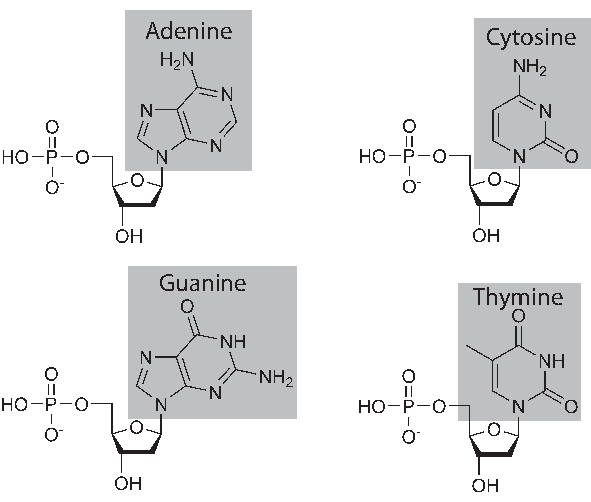
\includegraphics[width=\smallfigure]{\FIGPATH/Figures_Intro/nucleotides}
\caption[Nucleotides, the elementary subunits of DNA.]{
\label{fig:nucleotides} The four different nucleotides of DNA: Each nucleotide
consists of a phosphate group, the sugar desoxyribose and one of the bases adenine, 
cytosine, guanine or thymine.
 Source of images: Wikipedia.}
\end{figure}

Single stranded DNA (ssDNA) alone is not suitable as a storage medium for hereditary information 
because single phosphate bonds are not stable enough and a damaged single strand is hard to repair without a backup copy.
\nomenclature{ssDNA}{Single stranded DNA}
\nomenclature{dsDNA}{Double stranded DNA}
Both problems are solved elegantly by the ability of ssDNA to pair with a 
\emph{complementary} strand. The geometry of the bases 
adenine and thymine is such that they can form two hydrogen bonds, whereas
cytosine and guanine interact via three hydrogen bonds, cf.~\FIG{DNA_structure}. 
The interaction between these bases occurs only, if they are aligned in opposite 
polarity. Therefore a DNA strand binds 
selectively to a strand, the sequence of which is the complementary sequence in opposite
order. After base pairing, the double stranded DNA (dsDNA) winds into a double helix, which brings consecutive
base pairs closer together and shortens the duplex from 0.7~nm per base in single strand
to 0.34~nm in double strand. The double helix has an diameter of approximately 2~nm and a
helical pitch of about 10.5~bp or 3.5~nm. By base pair stacking, water
is driven out of the space between base pairs and the carbon rings of bases align, which 
is the major contribution to the DNA binding free energy. The DNA double helix is not completely
symmetric, meaning the two bases of a base pair do not form an angle of 180${}^\circ$. 
Thereby, dsDNA has a major and a minor groove, as illustrated in \FIG{DNA_structure}b.
\nomenclature{Stacking interactions}{Consecutive base pairs in dsDNA stack on top of each other
and thereby drive water out of the inter-base region. These stacking interaction are a major 
contribution to the DNA binding free energy\refpage}%

In contrast to ssDNA, damage to dsDNA is easy to repair. 
The complementary strands can serve as a template for reconstruction of a damaged strand
and for replication of the molecules. The stability of dsDNA and its potential to be repaired
enable cells to maintain genomes as long as $10^{10}$ nucleotides, resulting in molecules of 
macroscopic length.
\begin{figure}
\centering
  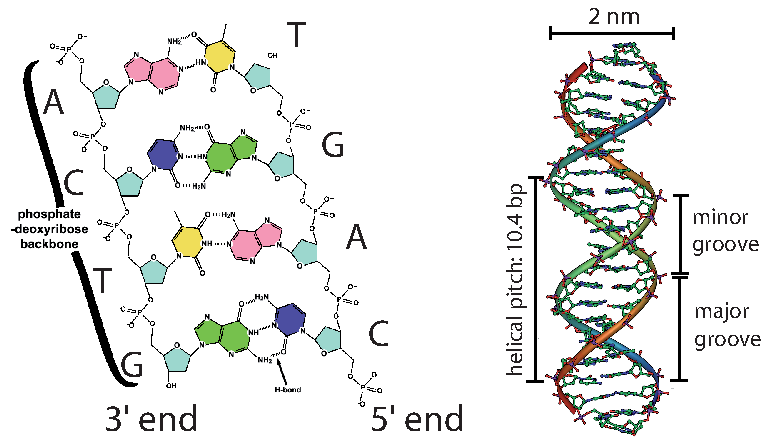
\includegraphics[width=0.7\columnwidth]{\FIGPATH/Figures_Intro/DNA_structure}
\caption[Structure of dsDNA]{\label{fig:DNA_structure} Left: Two oppositely aligned DNA strands
bind specifically to each other if their sequences are complementary, i.e. if
each base \basepair{A} faces a \basepair{T} and each base \basepair{G} faces a \basepair{C}. Hydrogen bonds
between bases are indicated by dashed lines. 
%Two complementary DNA strands thus form a ladder-like structure
%where the sugar-phosphate backbones form the stiles and the base pairs the rungs.
Right: The ladder-like structure compactifies further by winding into a double helix.
The pitch of the double helix 3.5~nm, which corresponds to $\approx 10.5$~bps. 
Since base pairs are not perfectly straight the helix displays a major and a minor groove.   
%The double helix is stabilized by stacking interactions between $\pi$-bonds of consecutivebases. 
Source of images: Wikipedia.}
\end{figure}


\section{Thermodynamics of DNA}
In the previous section we discussed how the chemical architecture of DNA makes it an
ideal carrier of genetic information. We will now turn to thermodynamic properties
of DNA which have implications for the ability of cells to read the sequence information from the DNA. 
Efficient information read out is possible only when the double helix is opened and the unpaired bases are exposed. Hence, the cell has to separate dsDNA locally into single strands at ambient temperature.
How this can be achieved is mainly determined by binding affinity of the two strands and their 
fluctuation properties, which therefore have been studied extensively, both
experimentally and theoretically. 

The basic ingredients to DNA thermodynamics are the free energy contributions of base pairing
and stacking interactions. Using these parameters, the properties of short 
molecules can be well understood with simple two state models. 
Subsequently we discuss the melting behavior of long molecules and calculate the 
partition sum of a dsDNA molecule within the framework of the Poland-Scheraga model.
%When studying repetitive DNA in chapter \ref{sec:DNA_sliding} we will generalize the 
%Poland-Scheraga model to incorporate non-native base pairings. 

\subsection{Binding free energies of double stranded DNA}
The dominant contributions to the binding free energy of double stranded DNA are
H-bonds between bases in Watson-Crick base pairs and the stacking
interaction between subsequent base pairs. The binding of the two strands goes along
with a significant reduction in entropy, since two floppy single strands are forced into 
a much more rigid double stranded conformation. 
Assuming constant specific heat $c_p$, the free energy of a particular structure is given 
by
\begin{equation}
\label{eq:DNA_free_energy}
\Delta G = \Delta H -T\Delta S,
\end{equation}
where enthalpies, entropies and free energies are measured with respect to the dissociated
case. To a good approximation, $\Delta H$ and $\Delta S$ can be calculated as sums from 
contributions of consecutive base pairs, such as \basepair{AG/CT}. Additional free energy contributions 
stem from penalties for mismatches and loops or the lack of stacking interactions at the first and last
base pair, often called initiation  and termination costs.
\begin{equation}
\label{eq:DNA_free_energy}
\Delta G = \Delta G_{init} +\sum_{basepairs} \Delta G_{bp} + \sum_{loops} \Delta G_{loop}+\sum_{mismatches} \Delta G_{mm}+\Delta G_{term}.
\end{equation}
Many of the parameters have been carefully measured and are reviewed by 
\citeauthor{SantaLucia_PNAS_98} in \cite{SantaLucia_PNAS_98} and 
\cite{SantaLucia_AnnRevBioPhys_04}. While the precise binding energies depend on at least two consecutive base pairs, a good
rule of thumb is that a \basepair{CG} base pair contributes approximately $3\kT$ and an \basepair{AT} pair
about $2\kT$ at physiological salt concentrations. The penalty for initiating a loop, that is interrupting base pair stacking, is typically between $3$ and $10\kT$. 
%In contrast to the base pairing contributions, the penalties to initiate 
%and terminate the helix are length independent and are hence of particular importance for short molecules (up to 30 bps). The
%shorter a molecule, the lower its melting temperature. 
Extrapolation formulas of the parameters to 
different salt concentrations are also available \cite{SantaLucia_AnnRevBioPhys_04}. The complete set of 
parameters has been fed into software packages that predict melting temperatures and
plausible secondary structures of short DNA oligonucleotides, see for example \cite{Zuker_NAR_03}.

\paragraph{Two-state models.} 
Short DNA oligonucleotides occur in essentially two different states. The two strands are either
dissociated and float freely in solution, or the two strands are bound in their most stable binding 
configuration since any suboptimal base pairing is unstable. 
For such molecules, it is particularly easy to predict their melting temperature. 
%The free energy difference of the double 
%stranded state compared to the dissociated state is given by
%\begin{equation}
%\label{eq:DNA_free_energy_incl_conc}
%\Delta G = \Delta H -T\Delta S,
%\end{equation}
%where $\Delta H$ is the binding enthalpy and $\Delta S$ the reduction in entropy. 
The melting temperature $\Tm$ is commonly defined as the temperature where half of the 
single strands are part of duplexes. Setting $\Delta G$ in \EQ{DNA_free_energy} to zero and accounting for the 
 total concentration of DNA strands $c_T$, one finds \cite{SantaLucia_PNAS_98}
\begin{equation}
\label{eq:DNA_two_state_Tm}
\Tm = \Delta H/(\Delta S+R \ln c_T),
\end{equation}
where the gas constant $R=1.9872\frac{\mathrm{cal}}{\mathrm{K\cdot mol}}$.
Due to significant contributions from terminal ends, the melting temperature of short 
molecules strongly depends on the length. At larger length (above 30 base pairs), the melting temperature
mainly depends on the bulk binding energy and hence on the \basepair{CG} content of the sequence. 
Melting temperatures range from $20\Celsius$ for very short (5 base pairs) sequences 
to $90\Celsius$ for long \basepair{CG}-rich molecules.

\subsection{\label{sec:DNA_melting}Denaturation of long DNA molecules}
The assumption that two DNA strands are either firmly bound in the most stable state,
or completely dissociated is not justified for long sequences. Long sequences might have 
regions with different \basepair{CG}-content that melt at different temperatures. Even 
homogenous molecules will once in a while open their double stranded structure locally and 
form denatured bubbles as illustrated in \FIG{DNA_melting_experiment}. Two-state models are therefore not suitable for long molecules, but 
many different configurations  including partly melted patches contribute significantly. The most
important experimentally accessible quantity is the degree of base pairing of the DNA strands, 
which can be monitored 
by the absorption of UV light. Unpaired bases absorb UV light more efficiently than bases 
stacked in the double helical conformation and any change in the absorption coefficient can be
directly related to the degree of base pairing $\Theta(T)$ between the two strands \cite{Wartell_PhysRep_85}. 
If the local \basepair{CG}-content is constant along the molecule, the derivative 
$-\frac{d \Theta(T)}{d T}$ of the fraction of bound base pairs $\Theta$ 
has a single peak. However, the \basepair{CG}-content of DNA varies considerably along the genome\footnote{
There are differences in \basepair{CG}-content between coding and non-regions, 
as well as between incorporated viral DNA and proper DNA.}. 
In this case, the differential melting curve has many peaks corresponding to
different regions of the DNA that melt at different temperatures. A typical melting curve is shown 
in \FIG{DNA_melting_experiment}.
\begin{figure}
\centering
  \includegraphics[width=\largefigure]{\FIGPATH/Figures_Intro/DNA_melting_experiment}
\caption[DNA melting curve.]{
\label{fig:DNA_melting_experiment} 
Left: With increasing temperature the double stranded structure of DNA is interrupted by 
denatured loops and the two strands eventually separate. \basepair{AT} rich regions tend to denature
at lower temperatures due to their smaller binding free energy. Left: The UV absorbance and the negative 
differential of the fraction of base pairs vs. temperature, see main text.
%The differential melting curve has multiple peaks, corresponding to different stretches of DNA that 
%denature at different temperatures.
Reproduced from \cite{Wartell_PhysRep_85}.}
\end{figure}

Attempts to describe the melting transition of DNA theoretically date back to the late 1950s and
resulted in a class of models that are now commonly referred to as Poland-Scheraga models 
\nomenclature{PS-models}{Poland-Scheraga models. A class of models for base pairing configurations of 
dsDNA\refpage}%
\cite{Zimm_JChemPhys_59, Zimm_JChemPhys_60, Poland_JChemPhys_66a, Poland_JChemPhys_66b} or Ising
type models. These models describe a particular configuration of the DNA by the set of base pairs formed. In general, 
base pairs can be formed between any two complementary bases on different strands 
as wells as within one strand, that folds back onto itself. The latter is particularly important for RNA, 
but is rarely relevant for two complementary DNA strands since a high 
degree of self complementarity within a single strand is unlikely. 
%It is further assumed that base pairs do not cross, \emph{i.e.}~denatured loops and double helical stems
%alternate along the molecule.
Poland-Scheraga models are usually restricted to native base pairs, \emph{i.e.}~only base pairs
that are present in the ground state are allowed. The restriction to native base pairs is a good approximation, since
stable base pairing requires several consecutive base pairs and the chance of finding two non-native complementary 
stretches that are several base pairs long is slim. A convenient way to denote a base pairing configuration 
of dsDNA of length $N$ is by an ordered subset of the integers $\cS={i_1, \ldots, i_m}\subset[1,\ldots, N]$, 
which corresponds to the base pairs present in the DNA duplex.
Since we are not interested in reproducing experimental data as faithfully as possible, but rather
seek generic explanations to general features of DNA denaturation, it is reasonable to simplify the free energy 
model. In the following, we assume that stacking interactions do not depend on the base pair type
and include them through a cost $\Eini^{0}$ for initiating a loop. Furthermore, we assume that 
the loop penalty is independent of the bases in the loop and only depends on the loop size.  
%\begin{figure}
%\centering
%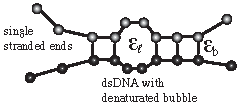
\includegraphics[width=\smallfigure]{\FIGPATH/Figures_Intro/PS_model}
%\caption[Poland-Scheraga model of base pairing.]{
%\label{fig:PS_model}Base pairing model of Poland-Scherage type. A base pairing
%free energy $\eps$ is assigned to each base pair of the sequence and a loop penalty
%to each internal loop, which interrupts the stacking of consecutive base pairs. Obviously, 
%the base pairing energy depends on the type of base pair (C-G or A-T) and the loop penalty
%might depend on the length of the loop and the sequence composition.}
%\end{figure}
The free energy model for a DNA configuration then simplifies to% (comp. \FIG{PS_model})
\begin{equation}
\label{eq:dna_melting_energy}
G[\cS]=-\sum_{i\in \cS} \eps(i) + \sum_{loops} \Eini(n_l),
\end{equation}
where $\eps(i)$ is the binding energy of base $i$ and $\Eini(n)$ is the free energy cost of a loop of size $n$.
However, even with this simple free energy model the explicit summation of all configurations 
is infeasible, since their number increases exponentially with the length.
Fortunately, there is a much more clever way to calculate the partition sum. Any allowed 
base pairing configuration is a sequence of double stranded stems and denatured
loops. Furthermore, the free energy of a particular configuration is a sum of local contributions 
from base pairs and loops. These properties allow the calculation of the partition function using recursion relations.
Let $Z_n$ be the partition function of a dsDNA molecule of length $n$, 
where the first and the last base pair are formed. $Z_n$ obeys the recursion relation
\begin{equation}
\label{eq:PS-recurrence}
Z_n=e^{\frac{\eps(n)}{\kT}} Z_{n-1}+\sum_{m=1}^{n-2}e^{\frac{\eps(n)-\Eini(m)}{\kT}} Z_{n-m-1},
\end{equation}
where the first term includes any structure that can be obtained by adding base pair $n$ to any configuration
in $Z_{n-1}$ and the sum includes all structures that are obtained when adding the base pair $n$
followed by a loop of size $m$ to any structure in $Z_{n-m-1}$.
%\begin{figure}
%\centering
%  \includegraphics[width=\smallfigure]{\FIGPATH/Figures_Intro/recursion_relation}
%\caption[Recurrence relation for the partition sum.]{
%\label{fig:recursion_relation} 
%Recurrence relation for $Z_n$.
%}
%\end{figure}
This recursion relation allows the calculation of the partition sum of arbitrary sequences of length $N$
in $\mathcal{O}(N^{2})$ steps. Similar recursion relations have been used to study the statistical physics
of RNA strands that fold back onto themselves \cite{Bundschuh_PRL_99, Flamm_RNA_00}.

\paragraph{The length dependence of the loop cost.}
When describing a dsDNA molecule by its set of base pairs it is implicitly assumed, that
all other degrees of freedom, \emph{e.g.}~the conformation of single stranded ends or denatured loops 
equilibrate rapidly compared to major rearrangements in the base pairing patterns. 
This results in a subtle dependence of the free energy of a loop on its length. Single stranded
DNA is rather flexible and changes its orientations typically every 2 to 3 base pairs, see \SEC{stretching_ssDNA}.
The possible conformations of ssDNA can therefore be mapped to the configurations of 
a random walk\footnote{Excluded volume effects of free single strand are not essential for the 
denaturation transition.}. The number of random walks increases as $\sim s^{n}$ with its length $n$. 
For ssDNA, $s$ has to be chosen such that $\ln s$ is the decrease in entropy when 
a single stranded monomer is forced into dsDNA. 
A denatured bubble in a dsDNA can also be described by a random walk, however, subject
to the constraint that the random walk forms a closed loop. This reduces the number of 
allowed configurations by a factor $n^{-c}$ giving rise to a loop penalty of entropic
origin of the form $c\ln n$ \cite{deGennes_79}. For ordinary random walks in $d$ dimensions $c$ has 
the value $d/2$. When self-avoidance is included, $c$ is given by $d$ times the Flory exponent $\nu$. 
At first sight this logarithmic correction to entropy appears to be of minor importance, but it is responsible
for a genuine denaturation transition in Poland-Scheraga models (see below). In particular,
a discontinuous transition requires $c\!>\!2$.
\citeauthor{Kafri_PRL_00} claim that $c$ is indeed larger than 2 when mutual 
excluded volume effects of different loops are taken into account \cite{Kafri_PRL_00}.  
In a nutshell the argumentation is
as follows: The denatured loops in a DNA molecule are not independent self-avoiding
polymer loops, but are linked by the double stranded stem to form a polymer network.
Excluded volume effects in a connected polymer network are stronger than for non-interacting loops, resulting
in a higher value of the exponent $c$. \citeauthor{Kafri_PRL_00} calculated a value of $c=2.15$ for DNA
denaturation, resulting in a discontinuous transition \cite{Kafri_EPJE_02}. 
However, the applicability of the scaling theory of polymer networks to DNA has been 
questioned \cite{Hanke_PRL_03, Kafri_PRLcomment_03}. The objection is, that denatured loops
are rare and far apart such that their interaction should be negligible. The rigid double stranded 
stems are essentially one dimensional objects, which are irrelevant for scaling. In any case, 
corrections to the loop exponent will only become important when studying DNA melting 
using extremely long molecules with very homogenous sequences.
For now, we treat $c$ as a variable and use a loop initiation cost of the form
\begin{equation}
\label{eq:loopcost}
\Eini(n)=\Eini^{0} -n\ln s + c\ln n,
\end{equation}
where $\Eini^{0}$ is a constant loop initiation cost due to the loss of base pair stacking
when a loop is formed. 

\subsection{\label{sec:DNA_melting_homo}DNA melting of homogenous sequences}
While the recursion relations are indispensable when studying the thermodynamics of
a particular sequence, they do not provide insight into the universal properties of DNA melting. 
To this end, we now demonstrate how the partition sum can be calculated in closed
form if the binding energy per base is the same for every base.  This might appear
to be a very restrictive and unrealistic assumption. However, we can coarse grain our 
description even further and lump a small number of bases together and treat them 
as a single entity. Given the sequence is random, the relative fluctuations of the 
binding energy of such ``super bases" become small. At the same time, each super base is likely to have a unique binding partner,
as assumed when choosing the set of allowed configurations. 
The assumption made is thus not that restrictive and the homogenous Poland-Scheraga 
model is adequate to study the melting transition\footnote{Obviously, this assumption
breaks down when macroscopic regions differ in \basepair{CG} content.
%, such as coding and non-coding DNA
}.

%If the loop penalty is independent of the loop size, the PS model is equivalent to an Ising model in
%one dimension. 
Poland-Scheraga models are essentially one-dimensional, similar to an Ising model.
It is well known, that one dimensional models do not exhibit 
genuine phase transitions. This fact is in conflict with the observed melting behavior of DNA and the 
apparent contradiction troubled (theoretical) physicists a while.
A genuine melting transition is only obtained if the proper dependence of
the loop cost on the loop length is included in the model.
The logarithmic term in \EQ{loopcost} introduces an effective long range interaction, that gives rise to  
an order-disorder phase transition in such one dimensional models \cite{Fisher_JChemPhys_66}.
The detailed thermodynamics of DNA was worked out by \citeauthor{Poland_JChemPhys_66a}
in the publications \cite{Poland_JChemPhys_66a,Poland_JChemPhys_66b} and later 
summarized in their book \cite{Poland_Scheraga_70}. We will now briefly summarize
the statistical physics of homogenous DNA following  \citeauthor{Poland_JChemPhys_66a}.
For a homogenous DNA molecule the recursion relation \EQ{PS-recurrence} simplifies to
\begin{equation}
\label{eq:PS_partsum}
Z_{n} = q Z_{n-1}+\sum_{m=1}^{n-2}\frac{qg^{2}s^{2m}}{m^{c}} Z_{n-m-1},
\end{equation}
where $q=e^{\frac{\eps}{\kT}}$, $g^{2}=e^{-\frac{\Eini^{0}}{\kT}}$ and the starting value of the recursion is 
set to $Z_1=q$. This recursion relation can be solved by $z$-transformation. The $z$-transform of
$Z_n$ is defined as $\Zh(z)=\sum_{n=0}^{\infty} Z_n z^{n}$ and is also known as generating function 
or discrete Laplace transform. Multiplying both sides of \EQ{PS_partsum} by $z^{n}$ and summing 
over $n$ yields after some algebra
\begin{equation}
\label{eq:PS_z_transform}
\frac{\Zh(z)-qz}{z} = q\Zh(z)+qg^{2}\Phi_c(zs^{2})\Zh(z),
\end{equation}
where $\Phi_c(z)=\sum_{n=1}^{\infty}\frac{z^{n}}{n^{c}}$ is the polylogarithm. \EQ{PS_z_transform} 
is readily solved for $\Zh(z)$
\begin{equation}
\label{eq:PS_Zh}
\Zh(z) = \sum_{n=0}^{\infty} Z_n z^{n}=\frac{qz}{1-qz-qg^{2}z\Phi_c(zs^{2})}.
\end{equation}
This $z$-transformed partition sum is nothing but the grand-canonical partition sum of a DNA
molecule coupled to a fictive nucleotide reservoir with fugacity $z$. 
The original partition sum of a molecule of length $N$ can now be recovered from $\Zh(z)$ by 
contour integration around the origin of the complex plane.
\begin{equation}
\label{eq:contour_integral}
Z_N = \frac{1}{2\pi i}\oint dz\: \frac{\Zh(z)}{z^{N+1}}=\frac{1}{2\pi i}\oint dz\: \sum_{n=1}^{\infty}\frac{Z_n}{z^{N-n+1}}
\end{equation}
The function $\Zh(z)$ is analytic everywhere, except on $[s^{-2}, \infty[$ and possibly at 
isolated singularities, \emph{i.e.}~zeroes of the denominator of \EQ{PS_Zh}. 
Having identified the singularities and branch-cuts, the contour integral can be evaluated by
calculating the residuals and the integral encircling the branch-cut, as illustrated in \FIG{contour_integral}.
A graphical solutions for zeroes of the denominator for different values of $c$ are given in \FIG{contour_integral}.
At low temperatures, that is large $q$, the denominator has a real root $\zc$.  
If $c>1$, this root merges with the branch-cut at some critical temperature and does not exist in
the high temperature regime.
\begin{figure}
\centering
  \includegraphics[width=\halffigure]{\FIGPATH/Figures_Intro/graphical_sol}
  \includegraphics[width=\halffigure]{\FIGPATH/Figures_Intro/contour_integral}
\caption[Contour integration in the fugacity plane.]{
\label{fig:contour_integral} 
Left: Zeros $\zc$ of the denominator of \EQ{PS_Zh} are given by the
intersections of $g\Phi_c(zs^{2})$ and $q^{-1}z^{-1}-1$ ($g$ and $s$ are set to 1 for simplicity).
%If $c<1$, there is a solution $\zc$ for every $q=e^{-\frac{\eps}{\kT}}$ and no melting transition exists (see main text).
Right: Contour integration in the fugacity plane. The contour integral around the origin is the sum 
of the residue at $z=\zc$ and the integral encircling the branch cut. For large $N$, the integral
is dominated by the residue.
}
\end{figure}
The partition function of a DNA molecule of length $N$ is therefore of the form 
\begin{equation}
\label{eq:residues}
Z_N =\frac{Res(\Zh(z), \zc)}{\zc^{N+1}} + As^{2N} \quad \mathrm{or} \quad Z_N =As^{2N},
\end{equation}
depending on whether the root $\zc$ exists or not. 
If $\zc$ exists, the fraction $\Theta$ of base pairs present in the
structure is given by the logarithmic derivative of $\ln Z_N$ with respect to $q$
%WOLFRAM ASKED FOR ADDITIONAL HINTS
\begin{equation}
\label{eq:fraction_basepairs}
\Theta=\frac{1}{N}\frac{\partial \ln Z_N}{\partial \ln q}= -\frac{\partial \zc}{\partial \ln q}.
\end{equation}
If the isolated singularity does not exist $Z_N$ does not depend on $q$ and $\Theta$ vanishes. 
The existence of $\zc$ is therefore connected to the phase where 
the two strands are bound and the temperature at which $\zc$ ceases to exist corresponds to the 
melting temperature $\Tm$. 
The order of the melting transition is 
determined by the value of the loop closure exponent $c$ \cite{Poland_JChemPhys_66b,Kafri_EPJE_02}: 
If $c\leq 1$, $\Phi_c(z)$ diverges as $z\to 1$, hence there is always a solution $\zc$ and no melting transition
exists. If $1\!<\!c\!\leq\!2$, $\Phi_c(z)$ remains finite as $z\to 1$ but approaches its limiting value
with infinite slope, resulting in a melting transition where $\Theta$ approaches zero as $T\to \Tm$ and the 
melting transition is continuous.
If $c>2$, $\Phi_c(z)$ tends to its limiting value with finite slope and $\Theta$ drops from
a finite value to zero at $T=\Tm$, giving rise to a first order melting transition.
Experimental melting curves of DNA are very steep, \emph{i.e.}~the fraction of bound bases vanishes 
very rapidly, and denaturation appears to be a first order transition. The additional contributions
to $c$ from loop interactions might therefore be relevant to reconcile the Poland-Scheraga models with experimental data. 
Available experimental data has been reexamined using $c=2.15$ instead of $c=3\nu\approx 1.8$, resulting in a smaller
estimate of the effective loop initiation cost \cite{Blossey_PRE_03}.

%REFER TO THE VALUE OF C

\section{\label{sec:DNA_mechanical_properties}Mechanical properties of DNA}
So far, we discussed the chemical and thermodynamic properties of DNA and 
neglected the organization of DNA in space. A typical human
chromosome is $10^{8}$~bp long, corresponding to a string of 3~cm in length. 
Forty-six of these strings have to fit into the cell's nucleus, which is only several micrometers
in diameter. Packaging and compactifying DNA is thus a nontrivial issue to cells, especially since
they have to keep their genome, or at least the relevant parts, accessible. This problem 
is addressed in the second part of this thesis. Obviously, the mechanical properties 
of DNA play an important role in DNA compactification and the dynamics of compactified DNA. 
During the last 15 years, it has become possible to study the mechanical properties of DNA by
 manipulating single molecules and measuring
their response to pico Newton forces. These single molecule force spectroscopy techniques provided
unprecedented insight into the static and dynamic properties of biological macromolecules 
and even allow to study cellular machinery such as polymerases or topoisomerases 
life on stage. The dynamics of repetitive DNA sequences
has also been studied using such techniques, which will be discussed in chapter \ref{sec:DNA_sliding}.
I will therefore give a brief overview
over such techniques and then discuss the mechanical properties of DNA.

\subsection{\label{sec:force_spectroscopy}Single molecule force spectroscopy}
At the molecular level, biological processes involve energy differences of the order of the thermal energy
$1\kT\approx 4\,pN\,nm$ and length scales on the order of nano meters.
To probe biological macromolecules mechanically, 
instrumentation is needed that is capable of applying forces in the pico Newton 
regime and measure distance with nano meter resolution. By now, a variety of different
techniques are available to achieve this feat and I will briefly discuss their basic mechanism
as well as their advantages and drawbacks. Atomic force microscopy is discussed in a little
more detail, since the slippage of repetitive DNA was detected using this technique
(see also \SEC{DNA_slippage_experiments}). For comprehensive reviews of the 
different techniques see for example \cite{Merkel_PhysRep_01, Bustamante_NMCB_00,Clausen-Schaumann_CurrOpChemBio_00}.

\paragraph{Optical tweezers.} 
When an object with an optical density higher than the surrounding  media is placed
in a non-uniform electric field, it feels a force towards the stronger field. This effect is exploited
in optical traps, where a small spherical bead is held in a laser focus. As soon as the bead is 
no longer centered in the focus, it experiences a restoring force. Although the explanation illustrated
in \FIG{force_spectroscopy} is not exactly applicable to beads of sizes of the order of a micrometer, it
conveys the essence of the method. The laser light is refracted by the bead and thereby transmits
momentum to the bead. If the bead is not centered, the laser intensity on the two sides of the bead
are not equal and hence the transmitted momenta do not balance, resulting in a net force towards
the focus. To study the response of a system to mechanical force, it is attached to the
bead and the exerted force can be determined by measuring the deviation of the bead from the 
trap center.  Interferometric methods allow to determine the bead position to nm resolution,
which for typical trap stiffnesses results in force resolution of pN and below.
The maximal forces optical traps can apply depend on the bead size and are in the range of 20 to 150pN.
One important application of optical tweezers has been the unzipping of single DNA molecules
\cite{Bockelmann_BiophysJ_02}, which is discussed in more detail below in \SEC{DNA_unzipping}. 
The motion of single processive molecular motors has also been studied using optical tweezers \cite{Clemen_BioPhysJ_05}.

\begin{figure}
\centering
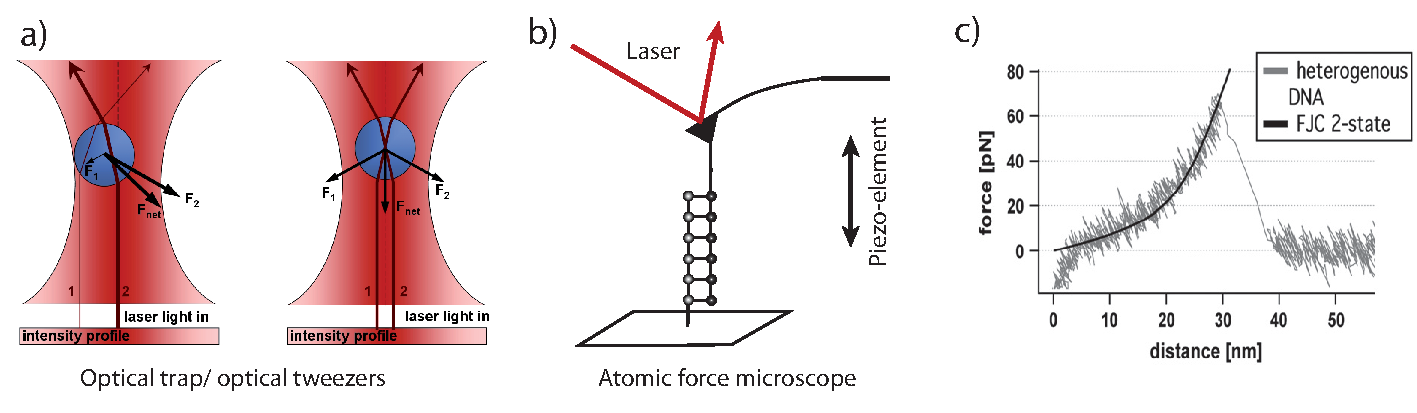
\includegraphics[width=\largefigure]{\FIGPATH/Figures_intro/force_spectroscopy}
\caption[Sketch of an optical trap and an AFM.]{\label{fig:force_spectroscopy}
Part a) Ray optics explanation of an optical trap. Image source: Wikipedia. b) Sketch of an AFM in a single molecule experiment. The different parts are extremely out of scale. c) A typical force-extension curve recorded with an AFM 
(taken from \REF{Kuehner_BiophysJ_07}).
}
\end{figure}

\paragraph{Magnetic tweezers.}
Similar to optical tweezers, magnetic tweezers exploit the fact that magnetic dipoles are attracted to high 
field regions and therefore experience a force in a gradient field. In addition to force, magnetic
fields exert torque on permanent magnetic dipoles. This opens up the possibility to twist biomolecules
by rotating the magnet that generates the field. The position of the beads can be detected using 
similar interferometric techniques as for optical tweezers, reaching nm resolution. The force 
can be sensitively controlled through the field gradient and forces as small as 10~fN can be applied. 
Magnetic tweezers have been used to study the stretching response of supercoiled DNA \cite{Strick_Science_96}
and to observe topoisomerases, the enzymes that disentangle DNA, in action \cite{Strick_Nature_00}.

\paragraph{Biomembrane force probes.}
Yet another technique of measuring small forces are biomembrane force probes. 
Small lipid vesicles or red blood cells are partially sucked into a micropipette to establish a 
well controlled tension of the vesicle membrane. The system to be studied is attached 
to the other end of the vesicle and pulled away. The deformation of the vesicle
can be related to the force applied to the sample. This technique has been used
for measuring the binding strength and kinetics of receptor-ligand systems \cite{Merkel_Nature_99}. 

\paragraph{Atomic force microscope.}
\nomenclature{AFM}{Atomic force microscope\refpage}
While optical and magnetic techniques excel at small forces with exquisite resolution, the realm 
of the atomic force microscope (AFM) are forces above 5pN. Among all force spectroscopy techniques,
the AFM has by far the greatest spatial resolution, which can be as good as the diameter of an atom.
Historically, AFMs were invented to map surfaces at atomic resolution, and only later became important tools
to study mechanical properties of biological macromolecules or molecular complexes. 
An AFM used for force spectroscopy consists of a tiny solid state cantilever with an even tinier tip. The substrate surface is mounted 
onto a piezo element which allows to move the sample with respect to the cantilever with extremely 
high precision. A force exerted on the cantilever will cause a slight bend in the cantilever. 
This minute deflection can be measured by shining a laser beam onto the reflective upper side of the 
cantilever, as sketched in \FIG{force_spectroscopy}. 
A deflection of the cantilever changes 
the reflection angle of the beam, which in turn can be sensitively detected by a split photodiode.
Since control and detection is done by fast electronic devices, 
the bandwidth of AFM measurements can be as high as 100kHz and
is limited by the viscous damping of the cantilever.

The substrate and the cantilever have to be prepared such that upon bringing the cantilever
in contact with the substrate, the sample attaches to both, the 
substrate and the cantilever. Often, the connection to the cantilever and substrate is 
established via well characterized and chemically functionalized linker molecules. 
Using linker molecules increases the distance of the sample from the surface and thereby reduces
surfaces effects. The sample density has to be chosen such that a single contact
between cantilever and substrate is more probable than multiple linkages. The substrate surface is then
retracted and the force is measured as a function of extension. Depending on the question 
to address, the force extension relation or the dependence of rupture forces on retract speed 
are informative quantities. 

\subsection{\label{sec:stretching_dsDNA}Stretching double stranded DNA}
%Among the first biomolecular applications of force spectroscopy was stretching dsDNA. 
%By now, the mechanical properties of DNA in different force and length regimes are fairly well understood.
\nomenclature{WLC}{Worm-like chain\refpage}%
On a microscopic scale, dsDNA is a very stiff polymer and thermal forces bend DNA
only on length scales long compared to the helical pitch  or even individual base pairs. 
To a good approximation, the DNA bendability is continuously distributed along the DNA
and the typical curvature radius is large compared to molecular dimensions. 
On the other hand, up to forces of about 50pN, dsDNA is virtually inextensible. 
Ignoring excluded volume effects the equilibrium conformations of DNA are therefore 
well described by the ensemble of inextensible
contour lines with a linear bending stiffness, a model commonly referred to as \emph{worm-like-chain
model} (WLC) \cite{Saito_JPSJap_66, Kratky_Porod_49}. The energy of a particular contour $\mathbf{r}(s)$ with a force $\mathbf{f}$ pulling
the endpoints apart is given by
\begin{equation}
\label{eq:WLC_energy}
E=\frac{\kappa}{2} \int_0^{L} ds\; \mathbf{t}'(s)^{2} -\mathbf{f}\cdot(\mathbf{r}(L)-\mathbf{r}(0)),
\end{equation}
where $\kappa$ is the bending stiffness and $\mathbf{t}'(s)$ denotes the derivative of the 
tangent vector with respect to the arclength $s$. To calculate the equilibrium properties of 
such a chain immersed in a heat bath, one would have to calculate the integral over all
possible paths $\mathbf{r}(s)$, which in general is infeasible. Some quantities, however, can 
be calculated exactly. In the absence of force, the 
most important exactly known quantity is the tangent correlation 
function at different points of the contour. 
\begin{equation}
\label{eq:WLC_tangentcorr}
\langle \mathbf{t}(s)\cdot\mathbf{t}(s')\rangle=e^{-\frac{|s-s'|}{\lp}},
\end{equation}
where $\lp=\frac{\kappa}{\kT}$ is called the persistence length. 
%Other exactly known quantities
%are the mean end-to-end distance or the radius of gyration \cite{WLC_lit}. Introduction of 
%self-avoidance renders the problem completely intractable.	
The persistence length is the length scale at which the correlations of different parts of the chain
decay and a molecule is considered flexible, if its total length is large compared to $\lp$. 
Conversely, a chain several times smaller than the persistence length is typically straight.
The persistence length of double stranded DNA under physiological conditions is $\lp=50\nm$.

\paragraph{Short molecules.}
Polymers that are short compared to the persistence length are often referred to as \emph{semi-flexible}.
The typical contours of these polymers are deviations from a straight line. If the straight
contour is the $z$-axis, the contour can parameterized by two single valued functions
$x(z)$ and $y(z)$. Furthermore, longitudinal contraction is only of second order, such that we can 
identify the arclength with $z$. Within this weakly bending approximation, the equation of motion of the
polymer is given by \cite{Barkley_JChemPhys_79, Wiggins_BiophysJ_98, Wilhelm_PRL_96}
\begin{equation}
\frac{\partial x(z,t)}{\partial t}=-\frac{\kT \lp}{\zeta} \frac{\partial^{4} x(z,t)}{\partial z^{4}},
\end{equation}
where $\zeta$ is the friction coefficient per length (analogously for $y(z,t)$). The eigenfunctions
of this equation are of the form $W_n(z)=a_1\sin k_nz+a_2\cos k_nz+a_3 \sinh k_nz+a_4\cosh k_nz$
with a discrete set of wave numbers $k_n$ fixed by the boundary conditions. The corresponding 
relaxation times are $\tau_n=\zeta/(k_n^{4}\kT\lp)$


\paragraph{Long molecules.} 
According to \EQ{WLC_tangentcorr} the correlation length of the tangent vectors $\mathbf{t}(s)$ along the backbone
is the persistence length $\lp$. Hence, a polymer that is far longer than its persistence length will form a 
random coil where the number of independent segments is given by $\sim L/\lp$. The diameter of the coil 
increases with length as $\sim \lp\left(L/\lp\right)^{\nu}$, where $\nu\approx 0.588$ is the Flory exponent. 
The end-to-end vector is a sum of independent increments and hence Gaussian distributed. The number
of possible chain configurations for a given end-to-end distance is maximal 
at zero separation and decreases rapidly as the ends are pulled apart. Entropy therefore
favors small end-to-end distances  and gives rise to a restoring force opposing stretching.
The force extension relation of a dsDNA molecule several micrometers in length
has been measured by \citeauthor{Smith_Science_92} using magnetic tweezers \cite{Smith_Science_92}.
At distances $\Delta r$ small to the backbone length the polymer 
responds like a linear spring with entropic spring constant $k=\frac{3\kT}{2\lp L}$.
The force-extension relation becomes non-linear as soon as the force exceeds $\kT/\lp$.
At very strong stretching, $\Delta r$ approaches the contour length and the undulations of the
of shorter and shorter wavelength are straightened out. The stretching force diverges 
quadratically as $\Delta r$ approaches $L$ \cite{Marko_Macromolecules_95}.


%CHECK WITH JULIA M
\paragraph{Overstretching DNA.}
DNA ceases to be well described by an inextensible WLC model at stretching forces of 
about $65\pN$, where the molecule suddenly extends by a factor of 1.7  
\cite{Cluzel_Science_96,Smith_Science_96}. The transition is reversible and very little hysteresis
is seen when the molecule is first overstretched and subsequently relaxed. Upon overstretching  
DNA changes from its ordinary structure called B-form to S-form. 
For this reason, the transition is called B-S-transition. Since the mechanical properties of
S-DNA are different from one single DNA strand, two separated single DNA strands, and ordinary B-DNA \cite{Cocco_PRE_04},
it is generally believed that S-DNA is double stranded but has a structure distinct from B-DNA.
The true structure of S-DNA is not completely resolved.
\citeauthor{Rief_NatStructMolBio_99}~report another conformational transition at forces of about
$150\pN$, which is irreversible on experimental time scales \cite{Rief_NatStructMolBio_99}. 
The force-extension trace of 
relaxation suggests that the two strands separate during the transition and only one single
DNA strand remains attached between the substrate and the cantilever. This force induced
unpeeling is strongly sequence dependent. 

\subsection{\label{sec:stretching_ssDNA}Stretching single stranded DNA}
\nomenclature{FJC}{Freely jointed chain} 
Single stranded DNA responds differently to stretching than dsDNA. Inspection of the 
chemical structure of ssDNA sketched in \FIG{DNA_structure} already hints at the great flexibility 
of ssDNA. The monomers are attached to each other via a single chemical bond, about which 
the bases can rotate and bend. In fact, ssDNA in solution reorientates about every two to three
bases. As opposed to dsDNA, the bendability of ssDNA is no longer continuously distributed 
along the chain but concentrated at the joints between the bases. A suitable model for such a system
is the \emph{freely jointed chain} (FJC) model which describes a polymer by a chain of rigid rods which are
connected at hinges. The length of single stranded DNA  corresponding to one segment of the FJC is 
about 1.5 to 2~nm. 
%There are many variants of this model, where the hinge itself can have a certain
%flexibility or allows only rotation at a fixed angle between two successive rods \cite{Livadaru_Macromolecules_03}.

Without a stretching force, the FJC model is equivalent to a random walk in space or, if mutual exclusion
of the monomers is accounted for, a self-avoiding random walk, as already discussed for the long
WLC polymer. At large stretching force, the response of the FJC differs from that of the 
WLC due to the fact that WLC polymer displays undulations at all wavelengths whereas the FJC
has a lower cut-off length given by the monomer length. The statistical mechanics
of a FJC polymer under tension is very simple and is equivalent to that of a paramagnet in an 
external magnetic field. The partition function of a single monomer of length $b$ is given by 
\begin{equation}
\label{eq:FJC_partfunc}
Z=\frac{1}{4\pi}\int d\phi \:d\!\cos\!\theta \:e^{-\frac{fb\cos\theta}{\kT}}=\frac{\kT}{fb}\sinh \frac{fb}{\kT},
\end{equation}
where the force is parallel to the $z$-axis. The partition function of a $N$-monomer chain is simply $Z^{N}$. 
From this, the force extension relation is readily calculated
\begin{equation}
\label{eq:Langevin}
\Delta r=-N\kT\frac{\partial\ln Z}{\partial f}= Nb\left(\coth \frac{fb}{\kT}-\frac{\kT}{fb}\right).
\end{equation}
As $\Delta r$ approaches $Nb$, the force diverges as $f \sim (Nb - \Delta r)^{-1}$. The functional
dependence of $\Delta r$ on $\frac{fb}{\kT}$ is known as Langevin function. For a thorough discussion 
of this and similar models, see \cite{Livadaru_Macromolecules_03}.

\subsection{\label{sec:DNA_unzipping}DNA unzipping}
Using single molecule manipulation techniques, one can unzip a single dsDNA. While separating the
two strands, the force needed for unzipping is recorded. Earlier  experiments
achieved a spatial resolution of hundreds of base pairs \cite{Essevaz-Roulet_PNAS_97}, 
which was later improved to tens of base pairs \cite{Bockelmann_BiophysJ_02}. 
To interpret these experiments, it is helpful to consider the time scales involved.
The unzipping speeds used in these experiments are on the order of $100\nm/s$, which corresponds 
to 300~bp per second. On the other hand, the intrinsic dynamics of base pair formation is faster than
$10^{6}$~bp per second \cite{Craig_71, Anshelevich_Biopolymers_84}. Hence, unzipping is 
slow compared to the base pair formation and the unzipping fork is essentially in equilibrium.
The opening of one base pair adds two bases to the single stranded part. 
The free energy per base of the single stranded DNA under tension can be calculated using 
\EQ{FJC_partfunc}.  The force adjusts itself such that this free energy equals half the binding free energy of a base pair. Hence, the binding free energy can be calculated from the measured force, 
yielding results in agreement with bulk thermodynamics.
The coupling of the dsDNA to the measurement device is soft, such that the fork
averages over many base pairs.  As expected, the estimated local binding free energies correlate 
with the \basepair{GC}-content of the sequence. Unzipping forces range between $10\pN$ for \basepair{AT} 
rich sequences to about $15\pN$ for \basepair{GC}-rich sequences. 

These unzipping experiments attracted the attention of many theoretical physicists which
studied the nature of the unzipping transition \cite{Lubensky_PRL_00} and in particular
focussed on the effect of sequence heterogeneity \cite{Lubensky_PRE_02,Cocco_PRE_02,Danilowicz_PNAS_03}.
The unzipping transition is a first order phase transition. The double helical state is 
stable at low force and the completely unzipped state is favorable at high force. If the experiments
are performed in the constant extension ensemble, the opening fork of the unzipped DNA
is the analog of a meniscus separating two phases. While the phase diagram is extremely simple,
the nature of the transition and the unzipping dynamics is sensitive to sequence disorder.
When unzipping homopolymers, every part of the molecule becomes unstable at the critical force
and  the number of unzipped bases diverges as $m\sim (f-\fc)^{-1}$ as the
transition is approached from below.  If the sequence consists of a random mixture of weakly and
strongly binding base pairs, the local binding energy fluctuates. Even though the energy landscape 
for unzipping is flat on average at the critical force, it fluctuates up and down like an 
unbiased random walk. Since the standard deviation of an unbiased random walk grows with square
root of the number of steps, the energy barriers the unzipping force has to overcome to proceed
$m$ bases are typically of height $\Delta E\sqrt{m}$, where $\Delta E$ is the difference in binding 
energy between the strongly and weakly binding base pairs.
It can be shown, that the number unzipped bases $m$ diverges 
quadratically as the transition is approached \cite{Lubensky_PRL_00}. 
Due to energy barriers on all scales, unzipping at constant force is often interrupted by long pauses
and the unzipping fork exhibits anomalous dynamics.
%Furthermore, the unzipping 
%is frequently interrupted by long pauses. Although on average unzipping
%is a downhill process, regions with very high \basepair{GC} content constitute barriers to unzipping. If the sequence
%was randomly assembled, the typical height of a barrier between two points grows with the square 
%root of the distance between these points, giving rise to an anomalous dynamics of the unzipping fork.
%WOLFRAM WANTS A DISCUSSION OF RANDOM FORCING VS RANDOM ENERGY LANDSCAPE
%Other researches investigated the dissociation kinetics of short dsDNA (10-30bps) molecules when
%applying shear forces with an AFM. 



  \chapter{Dynamics of repetitive DNA}
\label{sec:DNA_sliding}
At first sight DNA with repetitive sequences seems to be a rather artificial concept and 
one would not expect such DNA to be relevant in biology.  
Consider a DNA sequence such as \basepair{5'-CACACACACACACACACACA-3'} and its complementary
counterpart \basepair{3'-GTGTGTGTGTGTGT\-GTGTGT-5'}. In a randomly assembled sequence of typical genome length 
the probability to find this particular sequence
%, or any sequence consisting of a two nucleotide motive repeated 10 times or more, 
is small (there are $4^{20}\approx10^{12}$ ways to assemble
a 20~bp sequence, a mammalian genome is about $10^9$~bps long and hence the chance of occurrence is on the order of $10^{-3}$).
\nomenclature{Genome}{The complete hereditary information of an organism encoded in DNA} 
Nevertheless, perfectly periodic sequences, \emph{i.e.~}repetitions of short motifs of one to six nucleotides, 
are extremely common in eukaryotic genomes \cite{Ellegren_NRG_04} 
and account for up to 3\% of the human genome \cite{HumanGenome_Nature_01}.
This drastic overrepresentation of repetitive sequences cannot be
linked to any particular function, since 
most of these repetitive sequences have been found in non-coding regions of the
genome. Instead, what makes repetitive DNA
special compared to ordinary DNA is its much richer dynamics. While two complementary
single stranded DNA molecules with a sequence that is not particularly ordered form base pairs
only when correctly aligned, repetitive sequences can bind out of register and form
asymmetric loops as illustrated in \FIG{repetitive_DNA}. In particular, two complementary
repetitive single strands can slip, meaning they can bind to each other when locally shifted. 
This phenomenon of DNA-slippage is the key to understand the peculiarities of repetitive DNA.
In the following, we will outline the role of repetitive DNA in biology and discuss how it is linked
to human hereditary diseases. 

%One part of this thesis is a theoretical study of the dynamics of repetitive DNA. 
Using a simple model
of repetitive DNA we explore the potential of single molecule experiments to study the dynamics of DNA 
slippage. Our theoretical analysis suggests, that DNA-slippage can be probed by applying a shear force to a 
repetitive dsDNA. We find that the two repetitive DNA strands start moving relative
to each other when a sufficiently high force is applied. The observed sliding speed 
can be related to the microscopic dynamics of DNA-slippage. 
%The theoretical description of DNA sliding makes use of many appealing concepts
%from equilibrium and non-equilibrium statistical physics.  
Hence, a thorough understanding of this sliding motion might give insight into 
 the molecular basis of DNA-slippage and shed light on the evolutionary dynamics
of repetitive sequences. The peculiar properties of repetitive DNA could also be exploited
in nanotechnology as visco-elastic elements and force generators. 
Our theoretical study is complemented by a collaboration with 
 the lab of Prof.~H.E.~Gaub, where Ferdinand K\"uhner and Julia Morfill succeeded in 
measuring DNA sliding using an atomic force microscope. These experiments are also discussed briefly.

Not only the  dynamical properties of repetitive DNA are different from ordinary DNA, but also 
its equilibrium thermodynamics is richer. If two repetitive and complementary DNA strands
of different length bind to each other, they undergo an additional temperature driven phase 
transition before they separate into two single strands at high temperatures. 
This additional transition will be discussed at the end of this chapter.

\begin{figure}
\centering
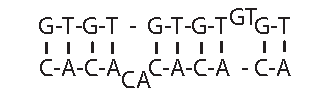
\includegraphics[width=\smallfigure]{\FIGPATH/Figures_sliding/repetitive_DNA}
\caption[Repetitive DNA has many binding configurations.]
{\label{fig:repetitive_DNA}
Two complementary DNA strands with repetitive sequence can bind in many different 
configuration, since strands are complementary even when locally shifted by in integral multiple of an 
repeat unit. In particular, repetitive DNA can form asymmetric loops and bulge loops, resulting in local strand slippage.
}
\end{figure}

\section{The biological role of repetitive sequences}
\nomenclature{SSR}{Simple sequence repeat. A multi-fold repetition of a short (one to six base pairs) motif\refpage}%
\nomenclature{Microsatellite}{Simple sequence repeat}%
\nomenclature{Short tandem repeat}{Simple sequence repeat}%
Repetitive sequences have first been observed in the early 80's \cite{Spritz_NAR_81} and since then 
have been found in every eukaryotic organism that was investigated. 
Repetitive sequences with short repeat motifs (one to six base pairs) are commonly 
called \emph{microsatellites}\footnote{DNA containing long repeated motifs forms 'satellite'
peaks in centrifugation experiments and such DNA was called satellite DNA. Later shorter and 
very short repeat motifs where observed and became known as mini- and microsatellites.}, 
\emph{simple sequence repeats} (SSR) or \emph{short tandem repeats}. To me, 
simple sequence repeat (SSR) appears to be the most natural name and I will try to stick to it.
Most of the simple sequence repeats are found in non-coding DNA and are believed to 
evolve more or less neutrally, that is the reproductive fitness of the organism is independent of length of the SSR. 
Only very little is known about possible functional roles of repetitive DNA, see below in \SEC{SSR_prokaryotes}. 
%While most SSRs appear to have no special function and are carried
%over time as ``selfish'' pieces of DNA, some people believe that SSRs have subtle roles in
%transcription regulation and might even be responsible for variability of socio-behaviorial traits
%\cite{Hammock_Science_05}. 
Within non-coding DNA, mono- and di-nucleotide repeats are
the most abundant, while within coding DNA, predominantly tri-nucleotide repeats are found.
Tri-nucleotide repeats constitute a special class of repeats, since the genetic code assigns amino acids to combinations of three bases, so called codons. 
\nomenclature{Genetic code}{Since there are more amino acids than bases, a multi-letter code is used to
store an amino acid sequence. Each amino acid is encoded by three consecutive bases, known as codons. 
The genetic code is redundant}%
A tri-nucleotide repeat in coding DNA therefore corresponds to 
a repeated amino acid in the protein. An extension or contraction of a tri-nucleotide repeat
results in the deletion or insertion of an amino acid but leaves other parts of the poly-peptide sequence 
unaltered. This is very different for most other repeat lengths, where expansions or deletions
result in frameshift mutations, \emph{i.e.~}the interpretation of the DNA sequence as three base
codons is changed for the entire part downstream of the repeat expansion. 
This most certainly results in a useless protein or premature termination of transcription. 
The special role of tri-nucleotide repeats and their 
relation to human hereditary diseases will be discussed in greater detail below.

\subsection{The number of repeats changes rapidly in evolution}
The key to understand the importance and ubiquity of SSRs
is the extraordinarily large rate at which the number of repeats changes from 
generation to generation. Although numbers have to be taken with care, rates
of contractions and expansions of SSRs in mammals can be as high as $10^{-2}$ per locus and
generation \cite{Dallas_MammGen_92}.
This is orders of magnitude higher than the typical rate for base substitutions which in mammals 
is about $10^{-9}$ per base and generation.	
This hyper-variability can be linked to a peculiarity of the mechanism by which DNA
is replicated prior to cell division. To replicate DNA, the double stranded molecule is
separated into two single strands by a helicase and the two single strands serve as
templates to which the complementary strands are added by the DNA polymerase. However,
the DNA polymerase operates only from the 5' to the 3' end. Therefore, only one strand,
the so called \emph{leading} strand, is copied continuously while the other strand, the \emph{lagging} strand, is
copied piecewise as illustrated in the upper panel of \FIG{replication_slippage}. 
The pieces of DNA that are added at a time
are known as \emph{Okazaki fragments}. The 5' end of an Okazaki fragment is fairly
unprotected and a couple of bases will frequently detach from the template strand by
thermal fluctuations. Whenever the 5' end of an Okazaki fragment happens to have a 
repetitive sequence, it is possible that it rebinds in a misaligned manner, forming a 
bulge loop containing one or more repeat units. 
\nomenclature{Okazaki fragment}{Piece of DNA polymerized continuously during piecewise replication of 
the lagging strand\refpage}%
If the DNA polymerase fills in the next Okazaki fragment while such a
bulge loop is present the number of repeat unit on the copied strand has changed with respect to the template strand. 
A bulge loop on the template strand  results in the deletion of one repeat, whereas a loop 
on the newly synthesized strand adds a repeat,
as illustrated in the lower panel of \FIG{replication_slippage}. 
%INDICATE TEMPLATE AND NASCENT STRAND IN FIGURE
\begin{figure}
\centering
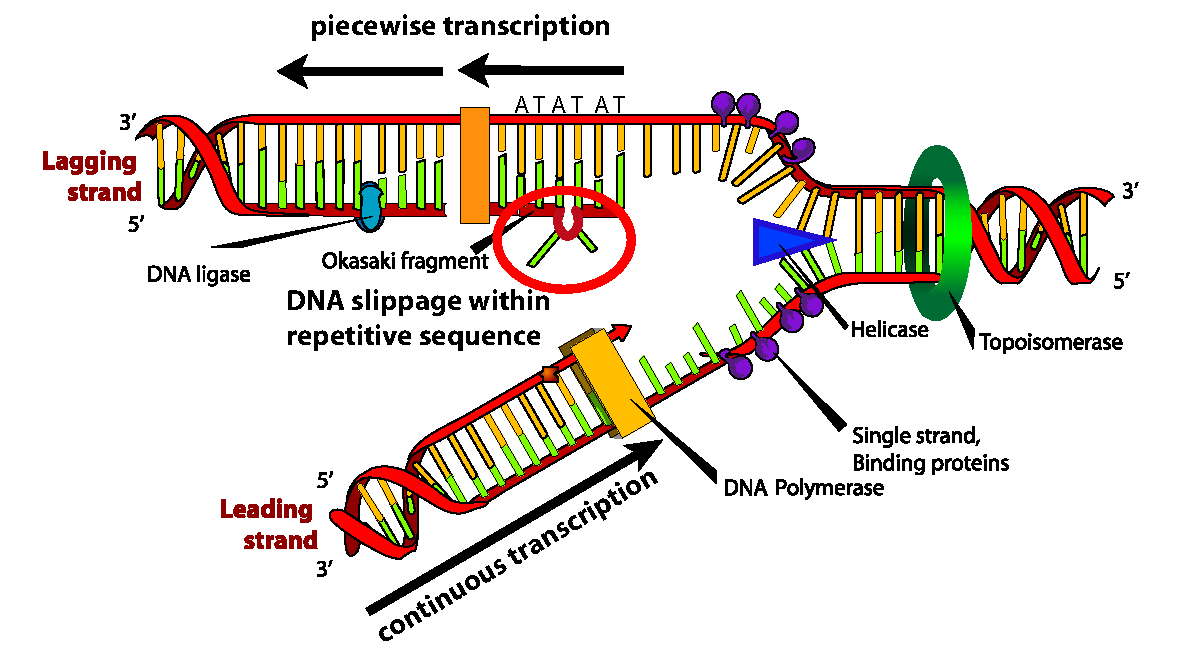
\includegraphics[width=\largefigure]{\FIGPATH/Figures_sliding/DNA_replication}
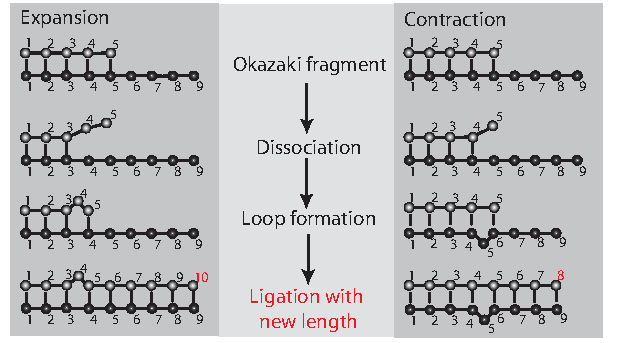
\includegraphics[width=\largefigure]{\FIGPATH/Figures_sliding/repeat_number_change}
\caption[Repeat number can increase or decrease during replication.]
{\label{fig:replication_slippage}
Upper panel: Replication of the lagging strand is done piecewise and the stretches replicated in one round
are called \emph{Okazaki fragments}. When an Okazaki fragment has a repetitive sequence,
the two strands can dissociate and subsequently rebind in a misaligned manner, as illustrated 
by the bulge loop inside the red circle. Image adapted from Wikipedia. Lower panel: Depending on whether the loop occurs on the template strand
or the new strand, the number of repeat units is increased or decreased in the copy.
}
\end{figure}

Energetically, SSR contraction is greatly favored over repeat expansion, since 
only one repeat unit has to open before a loop on the template strand can be formed, compared
to two repeat units that have to dissociate to from a loop on the nascent strand. 
Hence, one would expect SSRs to contract  and disappear quickly if the mutation mechanism was 
adequately described by the sketches in \FIG{replication_slippage}.
While this conclusion obviously contradicts
the abundance of SSRs in eukaryotic genomes, it explains the fact that SSRs are rare in prokaryotes and 
tend to contract during PCR, as discussed below in \SEC{PCR_slippage}.
The high ratio of expansion to contractions observed in eukaryotes is probably connected to the DNA mismatch repair machinery, which 
checks the double helical structure of the newly synthesized DNA. Only mutations
that escape this repair machinery or are falsely corrected persist to the next generation. Experiments in 
yeast have shown that a malfunctioning DNA mismatch repair system causes an increase 
of SSR mutations of 100-700 fold \cite{Strand_Nature_93}. These findings provide further indirect evidence that
misaligned rebinding during replication, \emph{i.e.}~replication slippage, is an important source of
SSR expansion and contraction. \emph{In vivo} rates of SSR evolution depend on a variety of different 
factors, most of which are still heavily debated in the literature. For a concise summary I recommend
\REF{Schloetterer_Chromosoma_00}.

\paragraph{SSR genesis and the length dependence of the mutation rate.}
The longer a SSR, the higher the probability that an open end during replication lies within
the SSR. One would therefore expect a linear increase of the expansion and contraction rate with
the number of repeats. Observations confirm a positive correlation between the 
repeat number and the mutation rate, the precise length dependence of the mutation rate, however,
is less clear and a large body of contradicting evidence exists (for a review, see \cite{Ellegren_NRG_04}).
Before a SSR can start growing by replication slippage, it has to contain at least two repeat
units.
% (If not convinced, try to redraw the replication slippage cartoons in \FIG{replication_slippage} for one, two and three repeat units.). 
It has been shown, that expansion of SSR does actually occur 
for SSRs as short as two units. It is generally believed that these initial seeds for SSR expansion are
assembled by chance.

\paragraph{Dependence of mutation rate on the repeat unit length.}
Another feature one would expect to have drastic effects on the SSR mutation rate, is the length of the
elementary repeat unit. The longer a repeat unit, the more bases have to dissociate before
DNA-slippage can occur. The activation free energy for DNA-slippage therefore increases
with repeat length and rates are expected to be small for SSRs with long repeat units. 
This reasoning is very well supported by \emph{in vitro} experiments (cf.~\SEC{in_vitro_slippage}),
but \emph{in vivo} evidence is less conclusive. Some experiments seem to confirm that
shorter repeat units mutate faster than long repeat units \cite{Lee_HumMolGen_99}. A bioinformatics
study also reports strongly decreasing mutation rates with repeat length \cite{Kruglyak_PNAS_98}. Repeated motifs
that are longer than five or six bases are not known to mutate significantly by replication slippage.

\paragraph{Length distributions of SSRs.}
A comparative study of the length distributions of SSRs of different repeat length in humans, mice, 
fruit-flies, and yeast revealed significant differences in abundance and distribution between different
organisms \cite{Kruglyak_PNAS_98}. In all cases, short SSRs are
most abundant. The longest SSRs are found in mice, but even for mice the frequency drops rapidly to zero 
beyond 40 repeats. The absence of very long SSRs is somewhat puzzling, since there appears 
to be a bias towards expansions of repeats\footnote{As noted above contractions are less costly energetically,
but more expansions seem to escape the mismatch repair machinery, resulting in an expansion bias.}. 
Furthermore, the mutation dynamics becomes faster as the length
increases. Very long SSRs are therefore expected. One possible resolution to this puzzle are point
mutations, which split a SSR into two smaller ones. The frequency of such a point mutation within one locus
increases with increasing length and thus provide a plausible explanation for stationary 
length distributions \cite{Kruglyak_PNAS_98}. However, one should keep in mind that many other influences, most importantly selection or unanticipated properties of the mismatch repair system, might be just as important
to understand SSR length distributions. 
%The issues, why short SSRs appear to expand but
%don't get arbitrarily long and how mutation properties differ between loci and across organisms
%is still far from resolved. 

The mechanism of SSR expansion discussed so far, \emph{replication slippage}, 
changes the length of an SSR usually by one repeat unit, sometimes by a few, but never by many.
However, the length of some special classes of SSRs tends to expand by a large number
of repeats in one generation. A common feature of such SSRs is their ability to form hairpins, 
\emph{i.e}~the ability of the single strand to fold back onto itself and form a stable structure.
Possible mechanism of SSR expansion due to hairpin formation are reviewed in 
\cite{Lenzmeier_CytoGenRes_03, Bzymek_PNAS_01}. Another source of length variations
of SSRs is unequal crossing-over during meiosis. When a diploid organism produces
haploid gametes, the genes on the chromosomes are reshuffled by building new chromosomes
out of pieces of the old ones. In repetitive parts of the genome, these recombination sites are 
ambiguous, which can give rise to two new chromosomes with SSRs of different length.


\subsection{SSRs are versatile genetic markers}
The human genome contains hundreds of thousands SSRs, each of which changes its length
with a probability of $10^{-6}-10^{-2}$ in each round of replication. The chance, that two humans
have the same set of SSRs is therefore negligibly small, even between closely related individuals. 
For this reason SSRs are ideally suited as genetic markers and have acquired great popularity
in phylogeny studies, paternity testing and forensic sciences. 
To measure the length of a set of SSRs, one exploits the fact that each SSR can be uniquely 
identified by its flanking sequences. A short fragment of DNA containing the SSR to be analyzed 
is cut from the sample using restriction enzymes that cut DNA specifically at the flanking sequences 
of the SSR. The short fragments are amplified by PCR and their length is measured using
gel electrophoresis. The resolving power of these
techniques is high enough to detect insertion and deletions of single repeat units \cite{Bennett_MolPath_00}. 
The great advantage of SSRs based genotyping techniques is the small length of the sequence 
fragments that need to be analyzed. Since short sequences can be efficiently amplified by PCR, 
minute DNA samples suffice for reliable data. 
Depending on the questions one wants to address, different genetic markers with different mutation
rates, chromosome type (autosomes, X-, or Y-chromosome) or flanking sequence are more 
suitable than others. 
\nomenclature{PCR}{Polymerase chain reaction. By PCR small amounts of DNA can be amplified rapidly and cheaply}
%Phylogenetic studies use the number of accumulated mutations as a molecular evolutionary clock
%to measure the time two species diverged from a common ancestor. For these applications a reliable 
%model and accurate parameters of SSR evolution have to be known to yield accurate predicitons.

\subsection{SSR expansion is related to hereditary diseases}
Most SSRs reside in non-coding regions of the genome and mutations of these SSRs
have little or no effect on the fitness of the individual. A special class of tri-nucleotide SSRs, however, occurs in 
coding regions or is part of introns, \emph{i.e.}~regions of a gene that are transcribed but spliced from the 
mRNA before translation, and mutations of these can lead to severely impaired phenotypes. 
Only tri-nucleotide repeats are found in coding regions due to strong selection against
frameshift mutations, which result by insertion or deletion of a number of bases that is incommensurate 
with three. Mutations of these tri-nucleotide SSRs are linked to a number of severe human hereditary
diseases, such as \emph{Huntington's}, \emph{fragile X} or \emph{Friedenreich's ataxia}.
These diseases fall into two different categories \cite{Reddy_COCEB_97}. 
The first class of tri-nucleotide related diseases is caused 
by expansions of \texttt{CAG} repeats that code for the amino acid glutamine. The most prominent
member of this class is Huntington's, which we will discuss in little more detail.
Huntington's is a neurodegenerative disease that develops gradually. At early stages, 
patients suffer from rapid uncontrollable movements. As the disease proceeds, 
patients loose virtually all motor control, including the ability to speak, eat, or facial expression. 
The gene containing the \texttt{CAG} repeat codes for the protein \emph{huntingtin}, whose
function is largely unknown. The number of repeats in healthy individuals ranges between 
6 and 34, people with 35 to 39 repeats have an increasing risk of developing the disease during
their lifetime and people with 40 or more repeats almost certainly suffer from Huntington's by the 
age of 40. Due to late onset of Huntington's disease, patients usually have children before
the disease is detected. The disease tends to becomes worse from generation to generation as the 
\texttt{CAG} repeat tends to grow longer and longer. The rate of elongation is correlated with 
the number of divisions in the paternal germ line \cite{Kandel_00}.
The molecular basis of the pathology of mutated huntingtin is still not completely 
resolved. The most popular hypothesis is, that proteins with a long poly-glutamine stretch tend
to aggregate and that those aggregates are toxic. Such aggregates have been found in the brains
of deceased patients. It is unclear, however, whether these aggregates are key to the pathology
or an unimportant byproduct \cite{Bates_Lancet_03}. In any case, it is extremely astonishing that 
the protein works fine with any number of glutamines between 6 and 34 and is almost certainly lethal 
with just 6 copies more.

The second class of pathological tri-nucleotide repeats are located in introns. In some
way or the other, the expansion of the SSR prevents transcription of the gene or the processing of the 
mRNA for translation into protein. 
Pathological expansions often reach repeat numbers as high as 2000, which is to be compared to the 
normal range of 5 to 50 \cite{Reddy_COCEB_97}. 
The most prominent member of this class is the fragile X syndrome causing mental retardation. 
Fragile X results from an expansion of a \basepair{CGG} unit beyond 200 repeats. 
The pathology of fragile X is believed to be related to methylation of \basepair{CG} di-nucleotides,
which might silence the transcription of the gene.



\subsection{SSRs in prokaryotes\label{sec:SSR_prokaryotes}}
In sharp contrast to eukaryotes, repetitive DNA is extremely rare in prokaryotes and
seems to occur only at loci, where there is a strong selective advantage to keep it. 
The prime purpose of SSRs in prokaryotes are \emph{contingency genes}, \emph{i.e.}~bacteria 
exploit the high mutation rate of SSRs to maintain genetic and phenotypic diversity within a 
population. Such diversity is essential to any organism subject to environmental 
changes, which may lead to extinction if not a small fraction 
of the population happens to be prepared for the new conditions \cite{Kussell_Science_05}.   
SSRs are exceptionally well suited for contingency genes, since SSR mutations are frequent and
lead to repeat number changes only. A change in repeat number differs from ordinary
base substitution mutations, since they are easily reversed. Assuming unbiased expansion
or contraction, there is a 50\% chance that a mutation is undone by the subsequent mutation, 
or put into more academic terms, random walks in one dimension are recurrent and almost surely
to return to the origin in finite time. This is very different for ordinary mutations, which correspond to 
a random walk in a very high dimensional space (every base can be of four different types), where
the chance of returning to a prior state is negligibly small. 

If there is a way to couple SSR contraction and expansion to switching genes on and off or 
to change protein function, rapid SSR mutations would result in phenotypic variation within 
populations and at the same time ensure easy recovery of temporarily switched off traits. 
Not surprisingly biology has found several ways to do so.
Among the best studied examples are contingency loci of human pathogens such as 
\emph{Haemophillus influenzae}\footnote{Although its name suggests that H.~influenzae
is the cause of the flu and hence a virus, H.~influenzae is a gram-negative bacterium. 
It was mistakenly associated with the flu until 1933.}
or \emph{Neisseria meningitis} \cite{Bayliss_JClinInv_01}. 
To evade the immune system,  these bacteria frequently exchange proteins in their outer 
membrane. This variability is often achieved by placing SSRs either in the promoter region or the in
coding sequence itself. A change in length within a promoter region can preclude necessary
interactions of transcription factors or destroy the RNA polymerase 
binding site. SSRs within the coding regions often cause frameshift mutations, which results 
in transcription termination or an ``gibberish'' mRNA. %In any case,  no functional protein is produced.


%\subsection{SSRs facilate homologous recombination}
%\cite{Napierala_JBC_02}



\subsection{\emph{In vitro} evidence for local strand slippage}
By now, it is fairly well established that replication slippage plays a pivotal role in the mutational
dynamics of SSRs. However, the change in repeat length from one generation to the next results
always from an interplay of replication slippage and the DNA mismatch repair machinery. Only
those mutations that escape mismatch repair or are falsely corrected can be detected. One way to study replication
slippage alone is to knock out the DNA repair machinery \cite{Strand_Nature_93}. Another way 
is to study DNA replication \emph{in vitro} \cite{Schloetterer_NAR_92}. Three examples of such 
experiments are described below.  

\paragraph{{\label{sec:PCR_slippage}PCR slippage.}}
The invention of the \emph{polymerase chain reaction} (PCR) was one of the most important steps
towards modern biotechnology. PCR allows to faithfully amplify minute amounts of DNA fast and cheaply.
During one cycle of PCR, the DNA template strands are separated by thermal denaturation, subsequently
the temperature is lowered such that short primer strands hybridize at the 3' ends of both strands.
A heat resisting DNA polymerase then extends the short primers and copies the template. By
multiple repetitions of these steps, the initial template is amplified exponentially.  
By now, PCR is a highly automated and very reliable technique. 
Only when amplifying repetitive DNA
the amplification is error prone \cite{Hauge_HumMolGenet_93, Murray_NAR_93}. The
product DNA is a mixture of the faithfully copied template DNA and DNA sequences where the
repetitive part has shortened by some repeat units. 
Why does the PCR loose repeat units while amplification?
%REDUNDANT....
Whenever the template strand has a repetitive sequence and the polymerase happens to fall
off the strand while transcribing the DNA, one strand can slip with respect to the other and 
form a bulge loop. Similarly to replication slippage \emph{in vivo}, the number of repeats changes 
if the polymerase resumes the replication while such a bulge loop
is present (cf. \FIG{replication_slippage}). 
Only contractions are observed due to the fact that the formation of a bulge loop has a lower
activation energy on the template strand.
Given a binding free energy per repeat unit $\eps$, contraction is more likely than expansion
by a factor of $e^{-\frac{\eps}{\kT}}$. 

\paragraph{\label{sec:in_vitro_slippage}SSR synthesis via DNA-slippage.}
\citeauthor{Schloetterer_NAR_92} succeeded in synthesizing repetitive sequences by exploiting 
DNA-slippage \emph{in vitro}. They mixed short repetitive DNA with DNA 
polymerase and the required nucleotides in a suitable medium. After some incubation time, 
they measured the length distributions of the DNA strands and found that the DNA
strands tend to grow \cite{Schloetterer_NAR_92}.  The elongation rate primarily depends 
on the length and the binding strength of the elementary repeat unit. 
Di-nucleotide repeats grow at a rate of 4 to 6 base pairs per minute while  tri-nucleotide repeats 
grow at a rate ranging from  0.5 to 3 base pairs per minute.
The elongation rate  of tri-nucleotide repeats correlates strongly with the number of 
\basepair{AT} base pairs in the repeat unit.

The observations can be explained by the following mechanism: 
The ends of the repetitive dsDNA undergo DNA-slippage and 
form a bulge loop which diffuses inside the double strand. The single stranded overhang
produced by this slippage event is then filled in by the DNA polymerase. When the
bulge leaves the double strand again, it
produces another single stranded overhang, which is then filled in by the
DNA polymerase. Since the rate of bulge loop formation depends exponentially on the 
binding energy of one repeat unit, di-nucleotide repeats are expected to grow faster than 
tri-nucleotide repeats. High \basepair{AT} content should also enhance slippage, as observed.

\paragraph{\label{sec:Poerschke}Evidence for chain sliding.}
In the 1970s, \citeauthor{Poerschke_BioPhysChem_74a} measured the hybridization kinetics
of short repetitive RNA oligomers \cite{Poerschke_BioPhysChem_74a}. 
When complementary strands are mixed, the rate limiting
step for hybridization is the formation of a critical nucleus of a few base pairs. Once such a 
nucleus is formed, the remaining bases rapidly close in a zipper-like manner. When sequences
have no particular order, a stable nucleus and subsequent zipping is only possible if the 
two strands are correctly aligned. This is very different for repetitive sequences,
since the two strands can bind with arbitrary shift relative to each other, see \FIG{Poerschke}a. 
Once such a misaligned duplex is formed, it is stable since both strands are bound by many 
base pairs. Hence, one would expect to find a large number of 
misaligned double stranded intermediates with a different number of base pairs.
The relaxation dynamics of these intermediates to the fully aligned state 
would further be expected to occur at markedly different rates, since 
the time required to dissociate the strands by thermal activation depends exponentially on the
number of base pairs. However, no such slow multi-exponential relaxation is observed 
\cite{Poerschke_BioPhysChem_74a}. 
\citeauthor{Poerschke_BioPhysChem_74a} himself provided a very plausible explanation 
for his results. As already discussed several times, repetitive sequences can form mobile
bulge loops. The propagation of a bulge loop from one end to another shifts both 
strands by the length of the loop, very much 
like a rug can be moved by propagating slack from one side to another, see \FIG{Poerschke}b. 
The energy cost for the nucleation of such a bulge is small and in particular does not depend
on the length of the molecule. 
\begin{figure}
\centering
\includegraphics[width=\smallfigure]{\FIGPATH/Figures_Sliding/Poerschke}
\caption[Evidence for fast chain sliding reaction.]{\label{fig:Poerschke}
Left: During the hybridization reaction of repetitive RNA oligonucleotides, many misaligned 
intermediates will be formed. Right: To explain the fast relaxation to the 
completely aligned state, \citeauthor{Poerschke_BioPhysChem_74a} suggested 
that the two strands can slide by the propagation of bulge loops from one end to the other.  
}
\end{figure}


\section{Force induced DNA-slippage}
The observations and experiments reported above provide good evidence that DNA-slippage
is indeed happening and that it plays a crucial role during SSR evolution.  
However, the evidence for DNA-slippage is more or less indirect and based on bulk 
observations. One goal of this thesis was to suggest experiments that allow to observe 
DNA-slippage in single molecules using modern force spectroscopy techniques (cf.~\SEC{force_spectroscopy}). 

We suggest, that  DNA-slippage can be induced by applying a shear force to 
repetitive DNA.  In a nutshell, application of a sufficiently high shear force fosters the 
formation of bulge loops on both unstretched ends of the DNA duplex, which then travel 
across the duplex and exit on the other side, as illustrated in \FIG{Poerschke}b. The duplex lengthens stepwise, 
where each step corresponds to an individual bulge loop,
the length of which can be one or several repeat units. We devise a theoretical model, that allows us
to predict experimental signatures and relate measurements to microscopic parameters of DNA-slippage.
Using kinetic Monte Carlo simulations, methods from statistical mechanics,
drift-diffusion, and reaction-diffusion theory, we uncover four different force regimes with
distinct characteristic behavior.
The model we use is simple enough to be amenable to analytic treatment, which
allows us to calculate the threshold forces and the average sliding speed exactly. 
We further investigate how this sliding behavior is affected by rare mutations that destroy
the perfect repetitivity of the sequence. Such mutations do not necessarily impede sliding,
but, depending on the frequency of such alien bases, delay the mechanical
response and require larger forces. 


%THEORY OF SLIDING
\subsection{Sliding dynamics of perfectly repetitive sequences}
In a typical force spectroscopy experiment, a force extension curve is recorded
until rupture. In such experiments, either the distance of the cantilever from the surface,
\emph{i.e.}~the extension of the sample, or the applied force is controlled, while the other is recorded.
Though in principle the same information can be gained from either of the two approaches,
there are significant practical differences between the two. 
The former is easier to implement experimentally, since distance can be precisely controlled
using piezo-elements. However, applying a constant force and monitoring extension is easier to interpret and handle analytically or numerically. In the following, we will study the response of repetitive dsDNA
to a constant shear force, as illustrated in \FIG{sliding_transitionstate}a.

\subsubsection{DNA sliding exhibits four different force regimes}
No matter how small forces are applied to the molecule, it will rupture eventually since the 
state of large separation has the lowest free energy. However, to separate the two strands, an activation
barrier has to be overcome. The height of this barrier depends on the applied force, as well as
on the internal dynamics of the system. In the case of repetitive DNA, the main question is whether
the two strands stayed in register or have shifted relative to each other before rupture.
Two possible transition states, \emph{i.e.}~the state prior to rupture, with and without sliding
are sketched in \FIG{sliding_transitionstate} b\&c. The free energies difference of these states to the
ground states are given by 
\begin{equation}
\label{eq:sliding_transitionstate}
\Delta E_{non-sliding}=N\left(\eps - f(\lss-\lds)\right) \quad \mathrm{and}
 \quad \Delta E_{sliding}=N\left(\eps - f(2\lss-\lds)\right).
\end{equation}
The parameters $\lss$ and $\lds$ are effective lengths of ssDNA and dsDNA chosen such that
the stretching free energy per base or base pair is given by $f\cdot\lss$ and $f \cdot\lds$, respectively.
Obviously, the transition state after sliding is always lower in free energy than the 
transition state, when both strands stick. At low force, however, even $\Delta E_{sliding}$
is positive and the dissociation of the two strands is a thermally activated barrier crossing process, no matter
which dissociation path is taken.
The rupture times are exponentially distributed with a mean time $\mrt$ that 
increases exponentially  with $\Delta E$ and hence exponentially with the length of the molecule. 
%Simulations confirm this reasoning, cf.~Fig.~2 in the publication reprinted in 
%\SEC{Neher_PRL_04}.
\begin{figure} 
\centering
\includegraphics[width=\largefigure]{\FIGPATH/Figures_sliding/transition_states}
\caption[Shearing repetitive DNA.]{\label{fig:sliding_transitionstate}
Part a): A dsDNA molecule sheared by a force $f$. Part b): When the DNA duplex ruptures without sliding, the last base pair before rupture will be a native base pair. Part c): If the two sequences
slide along each other, the transition state has a larger extension $L$, see text for details. 
Shorter duplexes rupture in a cooperative manner \cite{Strunz_PNAS_99}.
}
\end{figure}
The situation changes, when the force is increased to
\begin{equation}
\label{eq:sliding_fc_estimate}
\fc=\frac{\eps}{2\lss-\lds},
\end{equation}
where the $\Delta E_{sliding}$ ceases to be positive while  $\Delta E_{non-sliding}$
is still positive. If the duplex ruptures via sliding the dissociation should no longer be 
a thermally activated barrier crossing process but some sort of creeping motion from the ground state
to the transitionstate.  While sliding still involves local energy barriers such as bulge loop formation, 
there is no longer an extensive barrier. Hence, the mean rupture time no longer increases exponentially
with the length but is determined by how rapidly the two strands can move relative to each other. 
Simulations suggest, that $\mrt$ scales as $N^3$ at the critical force\footnote{
This force is actually slightly different from the expression given in \EQ{sliding_fc_estimate}
due to entropic effects.} $\fc$.
At forces above $\fc$, we observe a quadratic increase of $\mrt$ with $N$, see \SEC{Neher_PRL_04}.
How can the cubic and quadratic scaling be rationalized?
As suggested by \citeauthor{Poerschke_BioPhysChem_74a} the two strands can be shifted relative 
to each other by propagation of bulge loops from one end to the 
other end. But a loop that is nucleated at one end most likely leaves the duplex again at the same end.
It travels all the way to the other end only with probability $M^{-1}$, where $M$ is the  
number of base pairs (see \FIG{particles}a for illustration).
Since the nucleation rate of loops at the end is independent of the total length, the mobility of 
the two strands relative to each other is inversely proportional to the overlap length $M$.
This mechanistic explanation of strand mobility is consistent with the intuitive expectation, that
the friction coefficient of a one dimensional object should linearly depend on its length.
At the critical force, the nucleation rates of loops at stretched or unstretched ends are equal and 
the duplex shortens and lengthens at equal rates, resulting in an undirected diffusive motion.
Since the diffusion constant itself is inversely proportional to $N$, the time needed to overcome 
the distance $N$ increases as $N^{3}$. 
At forces above or below the critical force, bulge loops are 
nucleated more frequently on unstretched or stretched strands, respectively, than they are on the
opposite strand. This induces a directed motion either extending or contracting the duplex. The effective
drift velocity is inversely proportional to the overlap length $M$. The time required to overcome a
distance $N$ with a velocity proportional to $M^{-1}$ scales as $N^2$. 

This quadratic scaling does not persist to arbitrarily high forces, but crosses over to a linear
scaling. The threshold force $\fd$ for this crossover is given by the force, at
which also the $\Delta E_{non-sliding}$ becomes negative.
\begin{equation}
\label{eq:sliding_fc_unravell}
\fd=\frac{\eps}{\lss-\lds}.
\end{equation}
In this case, it is no longer 
energetically expensive to open base pairs from both ends. Since
consecutive opening of base pairs until rupture is faster than sliding, this 
mode of unravelling wins over sliding dynamically and repetitive sequences behave
similarly to random sequences. 

%%FIGURE illustrating particle anti-particle model?
\begin{figure} 
\centering
\includegraphics[width=\largefigure]{\FIGPATH/Figures_Sliding/particles}
\caption[Microscopic dynamics of DNA sliding.]{\label{fig:particles}
Left: A particle placed at site 1 will be exit at site $N+1$ rather than at site $0$ with probability $N^{{-1}}$. This 
can be seen from the steady state distribution resulting when particles are injected at a constant rate. 
The particle fluxes to the left or right are proportional to the slopes of the distribution, the ratio of which
is $N^{-1}$. 
Right: A particle-antiparticle model for bulge loop dynamics, see main text.
}
\end{figure}
On a macroscopic level, the sliding dynamics of the two strands is well described by a drift-diffusion
equation, where the drift and the diffusion coefficient are inversely proportional to the instantaneous
length $x$ of the overlap of the two strands at any instant. 
\begin{equation}
\label{eq:sliding_drift_diff}
\frac{\partial}{\partial t} \PD(x,t)=\frac{\partial}{\partial x} \left(\frac{D_0(f)}{x}\frac{\partial}{\partial x}-\frac{v_0(f)}{x}\right)\PD(x).
\end{equation}
By fitting the solution of this drift-diffusion
equation to the simulated rupture time distributions, we obtain the drift and diffusion 
coefficients $v_0(f)$ and $D_0(f)$ that
are independent of $x$ and depend on the force only. The dependence of the 
drift coefficient on the force can be understood by microscopic modeling of the bulge loop dynamics.
In essence, bulge loops on opposite strands behave as particles and anti-particles, cf.~\FIG{particles}b: They annihilate 
on encounter forming one double stranded repeat unit. Bulge loops can also be produced in 
pairs, when a spontaneously nucleated bubble separates into two bulges. The nucleation of bulge loops at the
ends is mimicked by a coupling to particle reservoirs, the density of which depends on the 
force applied to that particular end. The difference of particles and antiparticles fluxes is conserved and 
directly related to the sliding velocity of the two DNA strands: The sliding velocity is given by 
the difference of the reservoir densities on stretched and unstretched ends, 
divided by the length of the double stranded region. 
The reservoir densities are determined by the pseudo-equilibrium loop densities 
on stretched and unstretched ends, which be calculated from the partition sum of our 
model. These results and the corresponding plots are included in our publication entitled 
``Dynamics of Force-Induced DNA-slippage'' in \emph{Physical Review Letters} \cite{Neher_PRL_04}, which is reprinted in \SEC{Neher_PRL_04}. The details of the calculation of the partition sum, 
defect densities, and critical forces are presented in the \APP{DNA_partitionsums}.


%%EXPERIMENTS BY FERDI AND JULIA
\section{\label{sec:DNA_slippage_experiments}Single molecule experiments on DNA-slippage}
Our theoretical study was intended to trigger experiments that study DNA-slippage in single
molecules. We are very happy, that Ferdinand K\"uhner and Julia Morfill from the group of Hermann
Gaub were willing to perform such experiments and collaborate with us. 
The experiments show very clearly, that two strands with repetitive DNA can slide along each 
other once the applied shear force exceeds a certain threshold value. Sliding proceeds in  
stepwise manner and the observed steps are compatible with a shift by one repeat unit. 
The observations can be convincingly explained by the force induced formation of a bulge loop
which is propagated to the opposite end and thereby lengthens the duplex. 
The experiments were performed with two different sequences, a 10 fold repeat of 
\basepair{GTT} and a 15 fold repeat of  \basepair{GT}. 

In the vicinity of the threshold force $\fc$ for sliding, the sliding velocity is linearly related to $f-\fc$, 
and a sliding mobility $\mu$ can be defined via
\begin{equation}
\label{eq:sliding_mob}
v(f)=\mu \cdot(f-\fc)
\end{equation}
In the experiments the situation is reversed, as the velocity is imposed by the speed at which the 
cantilever is retracted and the force adjusts itself. Higher forces at a given speed correspond to 
higher ``friction'', \emph{i.e.}~lower mobility. The forces measured at different speed confirm an 
approximately linear relationship. As expected, the tri-nucleotide repeat
slipped slower than the di-nucleotide repeat.

The threshold forces observed in the experiments were considerably higher than expected
from theory. We expect this discrepancy to be the result of deformations of the duplex, which is
not accounted for by the theory. When a force is applied to one strand of dsDNA it will
take a few bases, probably of the order of one helical turn of the DNA, to distribute the force
evenly to both backbones. In this boundary region the double stranded structure is distorted. The
DNA sequences used are only 30~bps long and the two boundary regions take up the whole molecule. 
It is therefore not surprising, that the observed forces deviate from the theoretical estimates which
assume an undistorted structure. The short sequences also limited the number of possible
sliding steps to four or five\footnote{The terminal bases on both ends are opening and closing
very frequently and a duplex with fewer than 10~bp overlap rapidly dissociates under force before sliding
can be observed \cite{Strunz_PNAS_99}.}. Therefore, the predicted scaling behavior for the mean
rupture time could not be tested. Given the biological importance of repetitive sequences and 
putative applications as active nano-scale building blocks, mechanical properties and the 
kinetics of repetitive sequences continue to be an interesting and challenging field for 
single molecule studies. 
The publication containing these results is reprinted in \SEC{Kuehner_BiophysJ_07}
and the interested reader is referred to this publication for details \cite{Kuehner_BiophysJ_07}. 


%SLIDING WITH DISORDER
\section{\label{sec:sliding_disorder}DNA sliding in presence of sequence disorder}
After having discussed the sliding dynamics of perfectly repetitive DNA, the question whether
sliding is robust to mutations that destroy the repetitive pattern, arises naturally. We show that
DNA sliding persists even in presence of such disorder. However, the onset of sliding is delayed by a 
waiting time, during which all mutated base pairs are opened. 
 
To begin with, we simulated the response to a shear force of a molecule with repetitive 
sequence where once in a while a repeat unit has been exchanged by bases, that bind only to 
their native binding partner and not to any other bases in the sequence. We find, that 
the extension of the molecule remains constant for some time until suddenly a fairly normal 
sliding behavior sets in. The existence of some delay is obvious, since all mutated bases have to be opened before the molecule 
yields. But it is less clear how the state with all mutations open is established and how the delay
times are distributed. 
By monitoring the state of individual mutations during the waiting stage, we reveal that 
mutations open consecutively from both ends and that sliding starts, as soon as the last 
mutation has opened. The mechanism by which a mutation opens 
is illustrated in  \FIG{measuringrates}.


Since the mutations open from both ends of the molecule, the state of all mutations
can be described by the outermost mutations on both sides. If the total number of mutations
in the molecule is $M$, the outermost mutations perform a random walk on $[1,2,\ldots,M]$.
Sliding starts, when both of these random walkers meet, that is no more mutations are bound.
The rate, at which these random walkers hop, \emph{i.e.}~the outermost mutations open and close,
depends on the force and the spacing between mutations. At low force, the random walkers
are biased away from each other and mutations are preferentially closed. In this case, the 
waiting time before sliding increases exponentially with the size of the system. At high forces,
the mutations are preferentially open and the waiting time increases as a power law \cite{Schwarz_75}. 
We can therefore identify different dynamical regimes in the plane of 
mutation density and applied force, where rupture is fast or exponentially slow. 
%Mutations are driven open by the entropy gained when larger parts of the molecule are populated by 
%high loop densities. Conversely, mutations are kept closed due to the loss of base pairs and the
%formation of two permanent loops associated with the opening of a mutation. The mechanism, by 
%which mutations open and close is illustrated in \FIG{measuringrates}. The rates, at which the
%random walkers hop, \emph{i.e.}~at which the outermost mutations open and close, are therefore
%determined by the force applied and the spacing between mutations. Sliding starts, once the 
%outmost bound mutations coincide and the waiting time can therefore be modeled by the 
%first encounter of two random walkers in one dimension, where each site corresponds to one mutation. 
%When the two random walkers are biased away from each other, their typical time of first 
%encounter increases exponentially with the number sites, while they meet fast (polynomial) 
%if they are unbiased or biased towards each other \cite{Schwarz_75}. Indeed, the distributions
%of waiting times for evenly spaced mutations is well described by the random walker model. 
%Depending on the force and the mutation density, the waiting times either increase exponentially
%or polynomial with the length of the sequence, which allows us to extend the force regimes
%observed without mutations to weak sequence disorder. 

DNA sliding in presence of sequence disorder is treated in detail in our publication entitled ``DNA as a 
Programmable Viscoelastic Nanoelement'' in the \emph{Biophysical Journal} \cite{Neher_BioPhysJ_05}. 
Details of the two random walker model are presented in the supplementary material to this article. 
The publication and the supplementary are reprinted in \SEC{Neher_BiophysJ_05}.

%NANOSCALE BUILDING BLOCK
\section{\label{sec:nanomechanical_app}Repetitive DNA as a visco-elastic nanoelement}
In recent years DNA has become a popular material to build elaborate structures on a molecular scale
\cite{Seeman_Nature_03, Shih_Nature_04, Rothemund_Nature_06}. These applications exploit the
specificity of complementary base pairing to guide an ensemble of DNA strands with carefully designed
sequence into the desired conformation. DNA has also been used
to construct devices that undergo conformational transitions in response to a change in the
chemical composition of the environment. A very versatile approach is to construct strands that
bind competitively to a scaffold strand with different binding affinities. If the device is in a particular
conformation including a weakly binding strand, the addition of a more strongly binding strand 
will replace the weakly binding strand from the structure and, if designed properly, will result in the 
desired conformational change  \cite{Simmel_AppPhysLett_02}. Such competitive binding has also 
been used to reversibly cross-link acrylamid gels \cite{Lin_04}. Other structures are sensitive 
to variation of pH and such reversible pH-driven transitions have recently been coupled to an oscillatory
chemical reaction \cite{Liu_AngwChemie_03,Liedl_NanoLett_05}.

Here, we want to discuss briefly the potential of repetitive DNA in nano-mechanical applications.
Most applications mentioned above are rigid and conformational transitions occur only between 
well defined states or require the replacement of one strand by another. Repetitive DNA
might be useful when building more flexible devices that respond dynamically to mechanical forces. 
We have seen above that repetitive DNA lengthens by one repeat unit at a time, if subject to a 
sufficiently high shear force. Conversely, it contracts against a sub-threshold force until maximal
overlap of the two strands is reached. In this way, mechanical energy is reversibly transformed into
base pairing energy. Effectively, repetitive DNA acts as a contractile visco-elastic
element with a viscosity that can be programmed by choice of the length of the individual
repeat unit and the overall length of the molecule. The contractile force is determined by the
sequence composition. Such a visco-elastic element might find applications as a molecular tie-rope
that keeps a connection between two parts straight and at the same time adjusts its length. 
Another conceivable application is a molecular force sensor that responds to forces exceeding 
the threshold force. The read out signal could either be rupture or simply a relative
shift of the two strands measured by FRET. 
The sliding response can be delayed by mutations in the repetitive sequence that transiently
lock the two strands in a particular relative position. Cross-linking
 gels with repetitive DNA might also result in material with novel mechanical properties. 
A detailed characterization of the visco-elastic properties of repetitive DNA can be found
in the article reprinted in \SEC{Neher_BiophysJ_05} \cite{Neher_BioPhysJ_05}.

%INTERMEDIATE PHASE
\section{\label{sec:intermediate_phase}Intermediate phase in DNA-melting}
So far, we have been predominantly interested in dynamic features of repetitive
DNA, which proved to be much richer than DNA with sequences without a particular
order. Here, we show that not only the dynamics but also equilibrium properties of repetitive DNA 
are different from random DNA. 

The most prominent difference is, at least within Poland-Scheraga models,
 that the order of the melting transition is different for repetitive sequences than for ordinary sequences.
We have seen in \SEC{DNA_melting} that the order of the melting transition of DNA
depends on the entropy of denatured loops, which in turn is governed by the loop closure exponent $c$.
For random sequences, a loop of a given size at a given position corresponds to one
base pairing configuration. When sequences are repetitive, however, loops can be asymmetric
and the bases of a loop of size $n$ can be distributed between the two strands in $n+1$ ways.
This effectively reduces $c$ by one \cite{Poland_70}. 
Hence, no transition is observed if $c$ is smaller than 2, denaturation is continuous 
if $2\!\leq\! c\!<\!3$ and a first order transition is observed only, if $c\!\geq \!3$.
A brief discussion of physical values of $c$ was given in \SEC{DNA_melting}.

This argument can be formalized by calculating the partition sum of all possible pairings between
the two strands\footnote{Only pairings corresponding to alternating stems and loops (no crossing base pairs) 
are allowed. This is usually a good assumption due to steric constraints.}, as we already did to study DNA sliding. 
%Most of the theoretical
%studies of DNA denaturation consider only native binding of the two strands, partly because it captures
%the important features of the melting transition for most sequences, but also because
%it is easier to handle mathematically (for notable exceptions see \cite{Hill_JChemPhys_59,
%Garel_Biopolymers_04, Litan_JChemPhys_65}). For repetitive sequences, this simplification
%cannot be made and one has to generalize the model to all possible pairings between
%the two strands\footnote{Pairings are restricted to non-crossing base pairs, which 
%usually is a good assumption due to steric constraints.}.
%One finds, that repetitive sequences melt as ordinary sequences do, but the the loop
%closure exponent $c$ has to be replaced by $c-1$ \cite{Poland_70}. 
%Qualitatively, this is readily understood, since the bases of a loop of size $n$ can be 
%distributed in $n+1$ ways between the two strands, which a increases the weight
%of loops of this size by $\sim n$. Hence, no transition is observed,
%if $c$ is smaller than 2, denaturation is continuous if $2\!\leq\! c\!<\!3$ and a first order transition 
%is observed only, if $c\!\geq \!3$. The actual value of $c$ lies somewhere between 1.5 and 2.2, depending
%on how excluded volume effects are accounted for. A brief discussion of physical 
%values of $c$ was given in \SEC{DNA_melting}.
When the two strands have repetitive sequences, there is no reason to consider only strands of equal
lengths. Our study revealed an additional phase transition, which occurs when the two strands
are of different length. At low temperatures, the two strands form a rigid double
helix and the excess bases of the longer strand reside in a single stranded overhang. 
As the temperature rises, more and more of these unbound bases are absorbed into 
bulge loops within the double helix and the overhang becomes shorter. At a certain temperature
 all the bases are absorbed and the length of the overhang is no longer extensive. This transition
is a continuous phase transition which formally and conceptually resembles Bose-Einstein
condensation. The overhang corresponds to those particles that condense into the ground 
state, while bulge loops within the double helix correspond to populated excited states.
The intermediate phase persists in presence of weak sequence disorder. 
Our work on phase transitions in repetitive dsDNA is published
 in \emph{Physical Review E} \cite{Neher_PRE_06}, which is reprinted in 
\SEC{Neher_PRE_06}. 

\section{Conclusion \& Outlook}
The dynamics of repetitive DNA is a fascinating research area with many open questions 
remaining to be addressed. Due to their structural simplicity, such sequences are amenable to
methods from statistical mechanics and their generic properties can be elucidated 
without reference to a particular realization. We studied equilibrium and dynamical 
features of repetitive DNA using both analytical and computational tools. Many quantities such as
threshold forces, defect densities and phase diagrams can be calculated exactly within our model. 
When repetitive DNA  is sheared with sufficiently high forces the two strands start moving relative to each other. 
This motion is mediated by propagation of bulge loops from one end to the other, very similar to 
defect diffusion in crystals. The dynamics of the two strands can be described
by a drift-diffusion equation with drift and diffusion coefficients that are inversely proportional to 
the length of the double stranded overlap of the two single strands. The drift and diffusion coefficients 
can be related to the microscopic bulge loop dynamics using a reaction-diffusion model. These two 
different levels of description provide a link between the microscopic dynamics of a bulge loop inside 
double stranded DNA to the DNA sliding dynamics, that can be measured in single molecule 
experiments. First experiments confirm that two repetitive DNA strands slide relative
to each other when sheared \cite{Kuehner_BiophysJ_07}, but more experiments with longer strands are necessary to test the prediction
of different scaling regimes and to infer quantities such as bulge loop mobilities. 

From an engineering perspective, repetitive DNA has intriguing mechanical properties which could
be exploited in nano-scale devices. In essence, repetitive DNA acts as a visco-elastic element with 
a force offset. The characteristics of such an element can be chosen through sequence composition 
and length. By introducing mutations in the perfectly repetitive sequence, the response of the element
can be delayed in a controlled way.

The principle incentive to study repetitive DNA is to understand the evolutionary dynamics of simple
sequence repeats. Our research is focussed on microscopic properties of DNA under well controlled
conditions. On the other hand, the length distribution of SSRs in various 
genomes and the mutation dynamics \emph{in vivo} are being actively investigated. The gap between these too approaches is huge,
but I think that bridging this gap is not completely infeasible. After measuring the microscopic
rates in single molecule experiments, one can faithfully parameterize models for \emph{in vitro}
slippage as described in \SEC{in_vitro_slippage} \cite{Schloetterer_NAR_92}. By successively adding
a mismatch repair system, single stranded binding proteins, etc., it might be possible to understand
how these components work together \emph{in vivo}. 
Another possible role of DNA-slippage could be in prokaryotic transcription termination. 
Intrinsic terminator sequences in prokaryotes include a ``slippery" and weakly binding
poly-\basepair{A} stretch, usually 7 to 9 bases in length. Upstream of this of this slippery 
sequence is a palindromic sequence which forms a hairpin in the RNA transcript \cite{Hippel_Science_98}.
A popular hypothesis is, that this hairpin exerts a force on the RNA still inside the polymerase and
thereby terminates transcription \cite{Dalal_MCell_06}. The precise mechanism how this is happening is
unclear, but it is conceivable that the force exerted by the hairpin induces DNA-slippage, which then enables the
RNA to slide along the DNA out of the polymerase. It should be possible to address this question by pulling
on the nascent RNA strand as presented in \REF{Dalal_MCell_06} while having the polymerase transcribe 
repetitive and non-repetitive sequences with different binding energies.

%%%%PRL%%%
\cleardoublepage
\section[R.A.~Neher and U.~Gerland, \emph{Phys.~Rev.~Lett.}, {\bf 93}, 198102]{Dynamics of Force Induced DNA-slippage. R.A.~Neher and U.~Gerland, \emph{Phys.~Rev.~Lett.}, {\bf 93}, 198102, 2004}
\label{sec:Neher_PRL_04}
\clearpage
\addtocounter{page}{3}

%%%%FERDI_BIOPHYSJ%%%%%
\section[F.~Kuehner \emph{et al.}, \emph{Biophys.~J.}, {\bf 92}, 2491, 2007]{Force Induced DNA-slippage. F.~Kuehner \emph{et al.}, \emph{Biophys.~J.}, {\bf 92}, 2491, 2007}
\label{sec:Kuehner_BiophysJ_07}
\cleardoublepage
\addtocounter{page}{6}

%%%%%DISORDER_BIOPHYSJ%%%%
\section[R.A.~Neher and U.~Gerland, \emph{Biophys.~J.}, , {\bf 89}, p.~3846]{DNA as a programable visco-elastic nano-element. R.A.~Neher and U.~Gerland, \emph{Biophys.~J.}, , {\bf 89}, p.~3846, 2005}
\label{sec:Neher_BiophysJ_05}
\clearpage
\addtocounter{page}{9}

%%SUPPLEMENTARY MATERIAL
\subsection{\label{sec:biophysj_supp}Supplementary Material to \emph{Biophys.~J.}, {\bf 89}, p.~3846.}
\subsubsection*{Waiting Time Distributions}
\paragraph*{Two Random Walker Model}
We consider two random walkers in one dimension confined by two reflecting boundaries $M\!+\!1$ sites apart. Since we want to model the process of mutation opening preceding the sliding stage, we seek the distribution of times until encounter of both walkers, given they started at opposite boundaries. Their motion is equivalent to the motion of one walker on a triangular piece of the two dimensional square lattice.  The 2D walker on site $(m,n)$ corresponds the state, where the left 1D walker is $m$ steps from the left boundary and the right 1D walker $n$ steps from the right boundary (see Fig.~3, main text).  The 2D walker is reflected at the lines $m=0$ and $n=0$. The line, where both coordinates add up to $M-1$ corresponds to the cases, when both walkers in 1D meet and is therefore an absorbing boundary for the 2D walker. \\
The case, where the rates, at which the walker moves away and towards a boundary ($k_{in}$ and $k_{out}$) are independent of the site, has been solved by \citet{Schwarz_75} using the methods of image charges. \\ 
The quantity we are interested in is the distribution of the time of the first encounter of the two random walkers in 1D, or equivalently the lifetime distribution $P(\tau)$ of the random walker on the triangle. A walker sitting on any site $(m,n)$ with $m=M-2-n$ can hop on two absorbing sites with rate $k_{in}$. The distribution of $\tau$ is therefore given by
\begin{equation}
\label{eq:lifetime}
 P(\tau)=2k_{in}\sum_{n=0}^{M-2} \PD(n,M\!-\!2\!-\!n;\tau),
\end{equation}
 where $\PD(n,m;\tau)$ is the probability of finding the walker on site $(n,m)$ at time $\tau$, given it started at site $(0,0)$. In the following we derive approximations of the solution by \citeauthor{Schwarz_75}.

\paragraph*{Unbiased Hopping}
When the walker has no bias, e.g. $k_{in}=k_{out}=k$,  $\PD(n,m;\tau)$ is given by a sum of $4M^2$ terms. The solution by \citeauthor{Schwarz_75} can be rearranged to 
\begin{equation}
\begin{split}
  \PD(n,m;\tilde\tau)=&\frac{1}{M^2}\sum_{r,s=1}^{2M}e^{-2\tilde\tau M^2\left(2-\cos \frac{\pi r}{M}
-\cos \frac{\pi s}{M}\right)}(1-(-1)^{r+s})\\
&\cos\frac{\pi (2n+1)r}{2M}\cos\frac{\pi r}{2M}\cos\frac{\pi (2m+1)s}{2M}
 \cos\frac{\pi s}{2M},
\end{split}
\end{equation}
where  the time variable has been rescaled as $\tau=\tilde\tau M^2/k$. 
Only terms, where the argument of the cosines in the exponent are close to $0$ or $2\pi$, contribute significantly when $\tilde\tau>1/M^2$. After shifting the summation interval to $r,s=-M\ldots M\!-\!1$, significant terms are those the $r,s$ close to $0$. 
%Keeping only slowly decaying terms and rearranging the exponent, yields
%\begin{equation}
%\begin{split}
 % \PD(n,m;\tilde\tau)\approx&\frac{1}{M^2}\sum_{r,s=-M/2}^{M/2}e^{-4\tilde\tau M^2\left(\sin^2 \frac{\pi r}{2M}
%+\sin^2 \frac{\pi s}{2M}\right)}(1-(-1)^{r+s})\\
%&\cos\frac{\pi (2n+1)r}{2M}\cos\frac{\pi r}{2M}\cos\frac{\pi (2m+1)s}{2M}
 %\cos\frac{\pi s}{2M}.
%\end{split}
%\end{equation}
We can expand cosines with arguments $\frac{\pi r}{M}$ or $\frac{\pi s}{M}$ and keep only the first non-vanishing contribution.
\begin{equation}
  \PD(n,m;\tilde\tau)\approx\frac{1}{M^2}\sum_{r,s=-\infty}^{\infty}e^{-\tilde\tau\pi^2\left(r^2+s^2)\right)}(1-(-1)^{r+s})
\cos\frac{\pi (2n+1)r}{2M}\cos\frac{\pi (2m+1)s}{2M}.
\end{equation}
The range of summation can be safely extended to $\pm \infty$, as terms with big $r,s$ are exponentially small.
Plugging this approximation into \EQ{lifetime} yields, after some algebra, using similar approximations as above, 
\begin{equation}
 P(\tilde\tau)\approx\frac{2}{M^2}\sum_{r,s=-\infty}^{\infty}e^{-\frac{\tilde\tau\pi^2}{M^2}\left(r^2+s^2)\right)}\frac{(1-(-1)^{r+s})(r^2+s^2)}{r^2-s^2}
\end{equation}
Since only those terms with odd $r+s$ contribute, we change the summation variables to $2v=r+s-1$ and $2w=r-s-1$.
\begin{equation}
 P(\tilde\tau)\approx\frac{4}{M^2}\sum_{v=-\infty}^{\infty}e^{-\frac{\tilde\tau\pi^2}{2}\left(2v-1\right)^2}\frac{(-1)^{v}}{2v-1}\sum_{w=-\infty}^{\infty}e^{-\frac{\tilde\tau\pi^2}{2}\left(2w-1\right)^2}(-1)^{w}(2w-1)
\end{equation}
From this expression, we find a parameter-free lifetime distribution
\begin{equation}
  \tilde{P}(\tilde\tau)=M^2P(\tilde\tau)=-\frac{16}{\pi^2}\frac{\partial }{\partial \tilde\tau}Q(\tilde\tau)^2,
\end{equation}
where $Q(\tilde\tau)$ is given by
\begin{equation}
  Q(\tilde\tau)=\sum_{n=1}^{\infty}\frac{(-1)^ne^{-\frac{\pi^2 (2n-1)^2 \tilde\tau}{2}}}{2n-1}
\end{equation}
The approximations involved are justified for large $M$. However, even for small systems the 
agreement is excellent, as illustrated in \FIG{lifetime}.
\begin{figure}
\centering
\includegraphics[width=\smallfigure]{\FIGPATH/Figures_Supplementary/finite_size_J(t)}
\caption[Supp.: The lifetime distribution of two random walkers.]
{\label{fig:lifetime}The lifetime distributions for $M=3,5,10$ and the approximation for large $M$. The time axis is rescaled by $M^2$.}
\end{figure}

\paragraph{Biased Hopping}
When the rates $k_{in}$ and $k_{out}$ are different, there is no compact analytical expression for $\PD(n,m;t)$. However, the longterm behaviour of a such a biased random walker is easily understood. If $k_{in}$ is bigger than $k_{out}$, the walker approaches the absorbing boundary steadily. In the opposite case, the walker will stay close to the origin and only rare excursions will lead to absorption. Quantitatively, the hopping of the random walker on the triangle is well approximated by suitably chosen one-dimensional representation. To that end, we consider the probability to find the walker on the line $\nu$ steps away from the origin.
\begin{equation}
P(\nu;\tau)=\sum_{m=0}^{\nu}\PD(m,\nu\!-\!m;\tau)
\end{equation}
This amounts to projecting the motion of the random walker onto the symmetry axis of the triangle. 
The time derivative of this quantity is very similar to a one dimensional hopping process.
\begin{equation}
\begin{split}
\partial_\tau P(\nu;\tau)=-&2(k_{in}+k^{-})P(\nu;\tau)+2k_{in}P(\nu\!-\!1;\tau)+2k_{out}P(\nu\!+\!1;\tau)\\
&+k_{out}\left[\PD(0,\nu;\tau)+\PD(\nu,0;\tau)-\PD(0,\nu\!+\!1;\tau)-\PD(\nu\!+\!1,0;\tau)\right]
\end{split}
\end{equation}
The contributions from the boundary terms in the second line depend on the ratio of $k_{in}$ and $k_{out}$. 
When $k_{in}\gg k_{out}$ the walker rapidly approaches the absorbing boundary. The probability $\PD(0,\nu;\tau)$  of finding the walker on the reflecting boundary is small, as it is unlikely to make equally many steps with high rate and a low rate. In this case the boundary terms can be neglected entirely, so that the process reduces entirely to a 1D first passage problem. Using standard methods described in \REF{Gardiner_04}, one finds, that the mean first passage time 
\begin{equation}
\mt=\frac{M-1}{2k_{in}-2k_{out}}-k_{out}\frac{1-\left(\frac{k_{out}}{k_{in}}\right)^{M-1}}{2(k_{in}-k_{out})^2},
\end{equation}
increases linearly with the number of mutations $M$.  \\
In the opposite limit, when $k_{in}\ll k_{out}$, $\mt$ increases as $\left(\frac{k_{out}}{k_{in}}\right)^{M-1}$ with $M$. In this case equilibration along the line $n\!=\!\nu\!-\!m$ is fast compared to the lifetime of the walker and  $\PD(m,\nu\!-\!m;\tau)$ is almost independent of  $m$. Setting all terms $\PD(m,\nu\!-\!m;\tau)$ equal results in a 1D hopping process with site dependent rates. The mean first passage time of this process can be calculated in much the same way, yielding $\mt\sim \left(\frac{k_{out}}{k_{in}}\right)^{M-1}$ with polynomial corrections.
In summary, we find that, depending on whether the walkers have an inward bias, an outward bias or no bias, the mean lifetime scales linearly, exponentially or quadratically with time.
Since the force, at which $k_{in}$ and $k_{out}$ are equal, separates regimes, where the waitingtime increases exponentially with $M$ from  linear scaling, we call it critical
force $\tfc$ in the presence of mutations. The force  $\tfc$ 
converges towards the critical force $\fc$ in the limit of no mutations.


\subsubsection*{Measuring Hopping Rates}
So far, we have been concerned with the waitingtime distribution given a certain set of rates, at which mutations open or close. These rates depend on the applied force and on the distance between consecutive mutations and have to be determined in simulations. 

As long as there are at least two mutations bound, the dynamics of the opening and closing of mutations at one end is independent of the other end. To measure the rates for a given pair of force and mutation density, we used a simplified system,
where a dsDNA with equidistant mutations is fixed on the right hand side
and a force is applied to the first base of the upper strand 
(see \FIG{measuringrates}). This simplified system is useful, as finite size effects are smaller when one walker crosses $M$ mutations as when two walkers cross $M/2$ mutations each. Furthermore, subtleties of the mutual annihilation process do not enter the measurement.
\begin{figure}
\centering
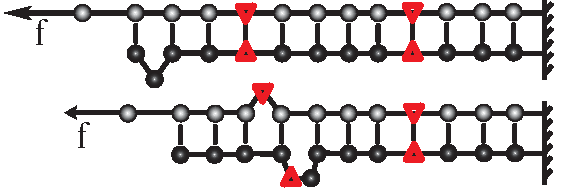
\includegraphics[width=\smallfigure]{\FIGPATH/Figures_Supplementary/Mutation_twostate}
\caption[Supp.: Measuring rates of mutation opening and closing.]
{\label{fig:measuringrates}Simplified system to measure the opening
and closing rates of mutations. The simulation starts from the ground state
with all bases bound. We determine the first-passage time distributions
of the opening of the rightmost mutation and fit these to a the first passage
time distribution of a random walker.}
\end{figure}
We measure the distribution of the time it takes to open the rightmost mutation for the first time and fit this distribution to the lifetime distribution of a random walker in one dimension between reflecting and absorbing boundary conditions. The rates $k_{in}$ and $k_{out}$ are fit parameters. This is done for a range of forces and mutation densities and the critical force $\tfc$ for a certain mutation density can be extract from the crossing of $k_{in}$ and $k_{out}$. To further pin down $\tfc$, we generated data for many force values slightly above and below $\tfc$ and fitted a linear relation for each rate to all data sets simultaneously. The crossing of the two resulting lines yield a robust estimate of $\tfc$. 
Using a system of $N=240$ basepairs, energy parameters $\eps=1.11\kT, \Eini=2.8\kT$ and different number of equidistant mutations, we determined $\tfc$ over broad range of mutation densities. The results are shown in Fig.~7(c) in the main text. \\
To check the reliability of the estimation of $\tfc$, we simulated waitingtime distributions by applying the force to both ends of the DNA and fitted the two random walker model to the waitingtime distribution. The force, where $k_{in}$ and $k_{out}$ coincide, reproduces the previously determined force $\tfc$. Furthermore, fitting the critical distribution (one fit parameter)  to the waitingtime distribution with yields best fits for $f\approx \tfc$. The absolute value of the rates shows slight dependencies on the length of the system (see below) and varies for fits to different setups. \\

\paragraph{Caveats of the Model}
Equilibration of the loopdensity is only possible by propagation of loops from the end beyond a newly broken mutation, or in other words by sliding the unstretched strand some distance $\Delta d$ inward. The sliding velocity, however,  is inversely proportional to the length of the strand. Therefore, equilibration will slow down breaking of mutations for supercritical forces deep inside the double strand and the linear dependence of the waitingtime on the number of mutations  will not persist for very large systems.

It is clear from the microscopic mechanism leading to breaking and opening of mutations (see main text and \FIG{loopdensities}) that the rates $k_{in}$ and 
$k_{out}$ depend on the force $f$. The rate $k_{out}$ also depends on the mutation density, since a great distance between mutations corresponds to a large entropy barrier for mutation closing, and hence a smaller closing rate $k_{out}$. The microscopic opening rate $k_{in}$ is expected to be more or less independent of the mutation density. When looking at the opening and closing dynamics of an individual mutation, this is what we observe.
However, the equilibration of loop densities after an opening or closing event takes some time. Therefore, successive microscopic opening and closing events are not entirely uncorrelated, which makes an unambiguous definition of the microscopic rates difficult. These correlations die out very quickly and it is still possible to describe the observed lifetime distribution with an uncorrelated random walker. The effective rates describing this motion both depend on mutation density and the applied force.

\begin{figure}[htb]
\centering
\includegraphics[width=\smallfigure]{\FIGPATH/Figures_Supplementary/loopdensities}
\caption[Supp.: Mutation opening is a trade-off between entropy and energy.]
{\label{fig:loopdensities}
Left: Illustration of how the density of loops on the strands depends on the state of the mutated bases in the sequence. In between bound mutations loops are rare, as the formation of a loop costs initiation energy and shortens the system. The same applies to the stretched strands outside bound mutations. The only part, where a significant number of loops can be found, is the unstretched strand outside the bound mutations. When a mutation is broken, loops  move across the mutation on the unstretched strand and locally both strands are shifted against each other. Thereby, the bases that previously formed the mutated basepair become permanently separated and the single strand part on the stretched strand grows.  
Right: To support the cartoon-like picture of part (a), we measured the time averaged loopdensity, conditioned on a certain mutation state.
Mutations are located at base 40 and 80, the parameters are $\eps=1.11\kT$, $\Eini=2.8\kT$ and $f=10.7 \pN$. We consider only opening of mutation from the left, i.e. the rightmost base is kept fixed, as in \FIG{measuringrates}. 
When all mutations are bound (upper panel), the loopdensity is high only on the unstretched
strand to the left of the mutation at position 40. When this mutation is broken (lower panel), loops can spread from the left end to the mutation at position 80, yielding a fairly constant density interrupted only by the permanent loop at the position of the mutated base. The hump to the left of the broken mutation on the unstretched strand and to the right of the broken mutation on the stretched strand indicate the position of the mutated base on the opposite strand. A loop already present on one strand renders unbound bases on the other strand more likely, as no additional loop initiation has to be paid. The vanishing loopdensity at the end of the stretched strand indicates unbound ssDNA. Observe, that this is the longer, the more mutations are broken. }
\end{figure}
\cleardoublepage
%%%%%INTERMEDIATE PHASE PRE%%%
\section[R.A.~Neher and U.~Gerland, \emph{Phys.~Rev.~E}, {\bf 73}, 030902(R)]{Intermediate phase in DNA-melting. R.A.~Neher and U.~Gerland, \emph{Phys.~Rev.~E}, {\bf 73}, 030902(R)}
\label{sec:Neher_PRE_06}
\clearpage
\addtocounter{page}{3}



  \chapter{Dynamics of nucleosomal DNA}
\label{sec:nucleosome}
Every cell of a multicellular organism carries the complete genetic information in its genome, 
regardless of its specific role as a part of the whole. Since different cells, \emph{e.g.}~a liver cell
and a neuron, need different proteins to function, cells are in need of a mechanism to control
which part of the genome is transcribed and which genes are silent. This not only applies to 
specialized cells of multicellular organisms, but to every cell we know. Even the simplest bacteria 
need to adjust their metabolism to the available nutrients and require different proteins at
different stages of the cell cycle. Regulation of protein production can occur either before
the gene is transcribed into mRNA, or target the process of the translation of mRNA 
into protein. 
To regulate transcription, the DNA contains short sequences that bind specifically to 
proteins called \emph{transcription factors} (TF). These transcription factors repress or
enhance the binding of the polymerase to the promoter, which is 
a prerequisite for transcription. The expression levels of the cell's genes is thereby 
controlled by the concentrations of transcription factors in the cell.

Eukaryotic cells suffer from an additional difficulty in achieving this feat. To fit their DNA into the 
cell's nucleus, the DNA needs to be strongly compactified. Due to this compactification the DNA is 
no longer freely accessible and transcription factor binding to DNA is to some extent precluded. 
The precise mechanisms of transcription regulation
in eukaryotes are unknown, but there is evidence that the compactified DNA is dynamic enough and 
exposes each part of its genome sufficiently often to allow for TF binding. 
On the other hand, cells exploit DNA compactification to
silence subsets of their genes and to determine cell fates during development. 
The dynamics of the elementary compactification unit of eukaryotic DNA, the nucleosome, has recently
been tested experimentally. In order to understand how the observed dynamics depends 
on various parameters of the system and what physical mechanisms might be responsible 
for the observed behavior, we investigate the dynamics of nucleosomes theoretically using
a simple model. Within our model, the dynamics of nucleosomes depends drastically on the 
polymer properties of DNA, which could also hold true for their dynamics \emph{in vivo}. 

In this chapter, I want to discuss the basics of chromatin structure and its implications
for gene regulation in eukaryotes. Then we will discuss two recent experiments, that studied the 
dynamics of nucleosomes and close with a discussion of our theoretical study.
%, that addresses the kinetics 
%of thermally activated DNA unwrapping from nucleosomes. 


%% CHECK NUMBERS IN FOLLOWING PARAGRAPH
\section{DNA compactification}
While bacteria have small genomes and avoid superfluous DNA, eukaryotes and in particular higher
multicellular organisms need more room to store their genetic information. In addition to the  
greater number of proteins that need to be coded, eukaryotes also tend to 
accumulate DNA that does not code for proteins and whose function is still unclear. In any case, 
the genomes of eukaryotes can be as big as a few gigabases for higher mammals. Even if broken 
up into several chromosomes, a DNA coil of that length is several tens of micrometers in diameter,
which is larger than the cell nucleus. Hence, there is a need for compactification, which is achieved
by an elaborate hierarchical organization of the DNA into chromosomes, as sketched in
\FIG{chromosome_organization}. 

At the lowest level of organization, the DNA double helix is wrapped
around a protein complex of cylindrical shape with a diameter of about 6~nm. This elementary packing unit is commonly 
referred to as a nucleosome. Its structure is known in exquisite detail and will be discussed in \SEC{nuc_structure}.
\begin{figure}
\centering
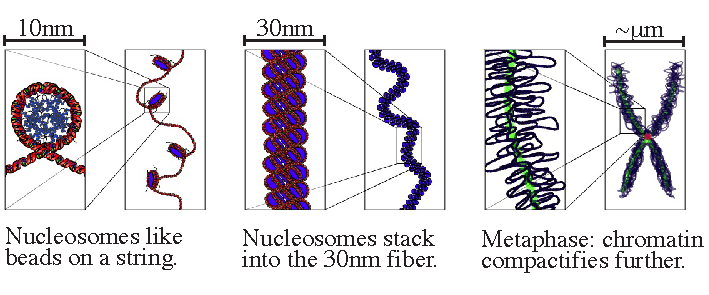
\includegraphics[width=\largefigure]{\FIGPATH/Figures_nucleosome/chromatin_structure}
\caption[Hierarchical organization of chromatin.]{\label{fig:chromosome_organization}
DNA is compactified into chromosomes in a hierarchic manner. See main text for details. 
%At the lowest level, DNA
%is wrapped around cylindrical proteins complex. The DNA-protein complexes are called
%nucleosomes. DNA with regularly spaced nucleosomes stacks into a thick and flexible fiber
%with 30nm in diameter. The structure at length scales between 100nm and $\mu m$ is less well known.
%Only during metaphase, dense chromosomes are formed. 
Image source: Wikipedia.}
\end{figure}
Nucleosomes are more or less evenly spaced on the genome with an average distance of about 30~nm. 
When stretched or in low salt conditions, this structure looks like a string of DNA with beads, 
the nuclesosomes, of about 10~nm in diameter. 
Under physiological conditions, this array of nucleosomes is further compactified to form a fiber  with 
30~nm in diameter, the structure of which is still subject to debate. The two competing models 
differ primarily in the geometry of the linker DNA between consecutive nucleosomes. In \emph{solenoid}
models, it is assumed that nucleosomes are arranged along a helix \cite{Finch_PNAS_76}, which 
requires the linker DNA between two nucleosomes to be strongly bent. For the second class of models,
it is assumed that the linker DNA is straight and crosses the center of the chromatin fiber. In 
these \emph{zig-zag} models two consecutive nucleosomes are assumed to lie on more or 
less opposite sides of the fiber \cite{Woodcock_PNAS_93}. Recently, the crystal structure
of tetra-nucleosomes was resolved, providing evidence for a zig-zag structure \cite{Dorigo_Science_04, Schalch_Nature_05}. A computational study also suggests
that the structure of oligo-nucleosomes is best described by an irregular zig-zag model \cite{Arya_PNAS_06}.
A more comprehensive overview and a survey of the current state of the debate is given in \REF{Woodcock_CurrOpStructBio_06}.
Due to its stacked structure without strong interactions along the direction of the fiber, the chromatin 
fiber is rather flexible and easily ripped apart by longitudinal tension. Stretching experiments on a single
chromatin fiber and comparison to an extensible worm-like-chain model suggest a persistence length 
of about 30~nm and a stretching modulus of 5pN \cite{Cui_PNAS_00}. This experiment further indicates, that 
the chromatin fiber disintegrates if tensions beyond 20pN are applied. 
Little is known about the intermediate levels of chromatin organization. It is believed, that the 30~nm fiber
forms large loops that are arranged on some scaffold, but evidence is sparse \cite{Alberts_02}. 
Only during cell division in the so called metaphase,  the DNA is packed into the dense structure known 
as chromosome\footnote{The name chromosome is derived from the greek word \emph{chromos} for 
color, since chromosomes are easily stained with dyes that bind to DNA.} that is large enough to be seen in
the light microscope. Our focus here is on the elementary packing unit, the nucleosome, and we will 
therefore describe the structure of the nucleosome in greater detail.

\subsection{\label{sec:nuc_structure}The nucleosome core particle}
While the structure of chromatin at larger length scales is still under debate, the nucleosome
 has been studied at atomic resolution. \citeauthor{Luger_Nature_97} succeeded 
in crystalizing the complex of histone proteins together with a short piece of DNA  wrapped around 
the protein complex 	and resolved the structure using X-ray scattering techniques. The first study achieved
a resolution of 2.8$\Ang$ \cite{Luger_Nature_97} and a subsequent experiment improved the resolution
to 1.9$\Ang$ \cite{Davey_JMB_02}. The structure of the nucleosome is illustrated in \FIG{nuc_structure}.
A piece of DNA, precisely 147~bps long, is wrapped around a cylindrical protein complex 1.7 times along 
a left-handed super-helical path. The pitch of this path is only 2.8~nm, such that the DNA comes very close
to itself along the super-helix. The protein complex has a diameter
of 6.5~nm and a height of about 6~nm. The cylinder is assembled out of four different  histone proteins
H2A, H2B, H3 and H4, each of which is present in two copies. 
These proteins form crescent shaped heterodimers (H2A-H2B) and (H3-H4), 
which are arranged such that they define a binding path for the DNA. 
\begin{figure}
\centering
\includegraphics[width=\largefigure]{\FIGPATH/Figures_nucleosome/nucleosome_crystalstructure}
\caption[Crystal structure of Nucleosomes]{\label{fig:nuc_structure} The nucleosome consists of 147~bp of DNA wrapped 1.7 times around
a complex of eight proteins. The two strands of DNA are shown in turquoise and brown. Only the 
main chains of the histone proteins are shown (H3: blue, H4: green, H2A: yellow, H2B: red).
Figure reprinted with kind permission by Nature \cite{Luger_Nature_97}.}
\end{figure}
The histone complex is positively charged and therefore attracts the negatively charged DNA. 
The DNA-protein interaction is concentrated in 14 well defined contact points located at positions where the minor 
groove of the DNA faces the protein core. Each contact points forms a variable number of hydrogen bonds with the
DNA. Due to the electrostatic nature of the protein-DNA interaction, 
the stability of nucleosomes depends on salt concentration.
With increasing salt concentration, nucleosomes disassemble into DNA and the histone core complex, before
the histone complex dissociates further into the dimers \cite{Schiessel_JPhysCondMat_03}.

The net binding free energy between DNA and the 
histones can be estimated using cleavage enzymes that cut DNA at specific sites. In these experiments,
cleavage sites are placed at different locations on the wrapped DNA and the reduction of 
the cleavage rate compared to free DNA is measured. By measuring this rate reduction,
one can estimate the fraction of time the DNA site is accessible to protein binding 
\cite{Polach_JMB_95, Polach_JMB_96, Anderson_JMB_00}, from which the free energy difference
of the wrapped and the unwrapped state is calculated. 
These cleavage studies also revealed a significant sequence dependence 
of the net binding energies, but as a rule of thumb, each contact point contributes about
1.5 to 2$\kT$ to the net binding free energy under physiological conditions. The net binding free energy is the amount 
by which the total interaction energy exceeds the free energy needed to force the DNA into
the strongly bent and clamped conformation when wrapped around a histone complex. 
The latter can be estimated as follows.
When only moderately bent, dsDNA is well described by a worm-like-chain model (WLC, comp. \SEC{stretching_dsDNA})  for semi-flexible
polymers with a persistence length of $\lp=50\nm$. Within the WLC model, the bending energy 
of the DNA in a nucleosome can be estimated to 
\begin{equation}
\label{eq:DNA_bending_energy}
E_{bend}=\kT\frac{\lp l}{2R^{2}}\approx 58\kT,
\end{equation}
where $R=4.3\nm$ is the radius of curvature of the DNA contour and  $l=43\nm$ is the length of the bend part.
%which is slightly shorter than the total length, since the last 3~nm on both strands are essentially straight.
This number for $E_{bend}$ should only be considered as an order of magnitude estimate, since 
it is not at all clear whether the WLC model is applicable to strongly bent DNA.
The estimate for the bending free energy leads to an estimate of the total interaction free energy of 
about $6\kT$ per contact point.  The binding strength and the bendability of the DNA are strongly
sequence dependent and special sequences, called positioning sequences, 
are known to bind preferentially to histones in a precise alignment.

\section{Gene regulation in eukaryotes}
In prokaryotes, the set of genes which is transcribed by the RNA polymerase into mRNA 
is determined by the concentration of transcription factors (TF) in the cytosol. 
The regulatory sequences to which TFs bind specifically are usually located
from 20 to a couple of hundred base pairs upstream of the gene and either enhance the 
binding of the polymerase to the promoter site by attractive interaction
or prevent the binding of the polymerase by steric hinderance. 
%Signals associated with different
%TFs can be logically combined by TF interaction and suitable architecture
%of the regulatory sequence \cite{Gerland_PNAS_02, Buchler_PNAS_03}.
These regulatory mechanisms are well established for prokaryotes, where the DNA is freely accessible
to passive TFs. 

Transcription regulation in eukaryotes is more complicated and many additional stages of regulation exist. 
The regulatory sites for a specific gene can be far away from the site where transcription starts and many more
signals are integrated to determine whether a gene is to be silent or not. The general picture of eukaryotic 
gene regulation is far from complete. Nevertheless, TFs have to find their binding sites,
even if they are hidden by nucleosomes. The comparatively small net binding 
energy of nucleosomes led to the hypothesis, that transient unwrapping of DNA from the histone complex
driven by thermal fluctuations could suffice for reliable gene regulation \cite{Polach_JMB_96}. 
\citeauthor{Polach_JMB_96} coined the term \emph{site exposure mechanism} for this tentative 
mode of gene regulation. The mechanism is illustrated in \FIG{site_exposure_mechanism}a. 
\begin{figure}
\centering
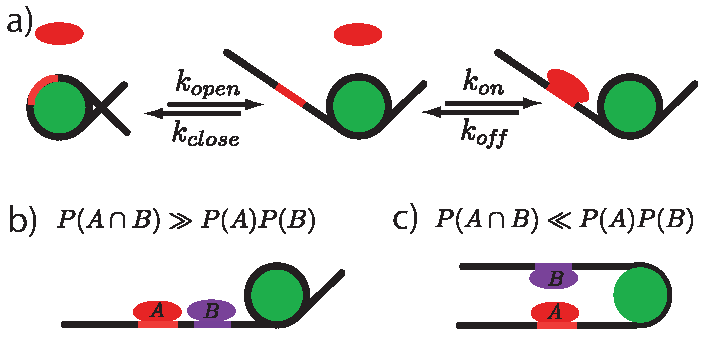
\includegraphics[width=\smallfigure]{\FIGPATH/Figures_Nucleosome/site_exposure_mechanism}
\caption[Site exposure mechanism]{\label{fig:site_exposure_mechanism}
Site exposure mechanism for protein binding to nucleosomal DNA.
Part a): Before the protein (red blob) can bind to its binding site (red), the DNA (black) has to detach from 
the histone complex (green). 
Part b\&c): Nucleosomes can mediate transcription factor interactions, see main text. 
%If two binding sites are located on the same side of the nucleosome dyad, their joint
%binding probability is greater than the product of the individual binding probabilities. 
%Part c): The converse is true, if the binding sites are located on opposite ends of the nucleosome,
%since unwrapping the last DNA turn is more costly than the first 0.7 turns due to the lack of electrostatic
%self repulsion of DNA.
}
\end{figure}
The site exposure mechanism allows to tune the binding affinity of a TF
 by the location of the binding site inside the nucleosome, the further away a site is from the 
entry or exit point, the harder it is to access. Indeed, it has been shown that the positioning
of nucleosomes along the genome is carefully controlled \cite{Segal_Nature_06}, which might be 
related to the tuning of binding affinities of TFs to their sites. The nucleosome can also be exploited
to mediate indirect interactions between TFs, see \FIG{site_exposure_mechanism}b\&c.
If two binding sites are located on the same side of the symmetry point of the nucleosome, exposure
of the binding site further inside the nucleosome implies the exposure of the other. Hence, the
joint binding probability is higher than the product of the individual binding probabilities, which is
equivalent to cooperative binding of the TFs. This type of nucleosome mediated TF interaction has
been shown to be a functional mode of gene regulation \emph{in vivo} \cite{Miller_MolCellBiol_03}.
In the opposite case, where the two sites
are at different ends of the piece of DNA, simultaneous binding is disfavored. To rationalize this, recall that
DNA is highly charged. In a nucleosome, DNA is wrapped 1.7 times along a helical path such that the  
DNA comes very close (a few \Ang) to itself for 0.7 turns. Due to self-repulsion of DNA, the first
0.7 turns are rather easy to unwrap, while the final turn is much more stable since self repulsion is
lacking. Two binding sites on opposite ends of the DNA are usually individually accessible by unwrapping
less than 0.7 turns of DNA, however, when exposing both of them simultaneously only little DNA remains
wrapped and one has to compensate the lacking self-repulsion. This gives rise to a joint binding probability
that is less than the product of the individual binding probabilities, equivalent to repulsive interactions. 
However, in order to be feasible, the site exposure needs to be fast. The remainder of this chapter will
address kinetic aspects of site exposure. Before presenting our theoretical study, 
I will discuss recent experiments, that study the dynamics of single nucleosomes  \emph{in 
vitro}.

\section{Experiments on single nucleosome dynamics}
A set of experiments addressing the dynamics of nucleosomes was performed by 
Gu Li in the group of Jonathan Widom. To study the fluctuation properties of DNA 
wrapped around a histone complex, they labeled a 147~bp long positioning sequence
at one end with a green fluorescent dye. 
In addition, they labeled the appropriate histone protein with a red dye, such that the two dyes
are in very close proximity when the DNA is fully wrapped around the protein complex. The two dyes used
are an efficient FRET pair, \emph{i.e.} the excitation energy can be transferred without radiation
from the green to the red dye via a dipol-dipol interaction. The efficiency of this energy transfer
decreases with the distance $r$ between the dyes as
\begin{equation}
\label{eq:FRET_efficiency}
E_{FRET}\sim \frac{1}{1+(r/R_0)^{6}},
\end{equation}
where $R_0$ is the separation at which the $E_{FRET}$ is half its maximal value. 
\nomenclature{FRET}{F\"orster Resonance Energy Transfer\refpage}%
\nomenclature{FCS}{Fluorescence Correlation Spectroscopy}
This distance is known as the F\"orster radius  and is usually on the order of a few nanometers. 
The FRET efficiency drops from near to one to negligibly small values in a
very narrow range surrounding $R_0$, which makes FRET an extremely sensitive distance measure.
The arrangement of FRET pairs on the nucleosome as realized by \citeauthor{Li_NatureStructMolBio_04}
allows the detection of the state of the nucleosome with optical means. 
In one publication \cite{Li_NatureStructMolBio_04}, \citeauthor{Li_NatureStructMolBio_04} convincingly showed, 
that the outermost part of the DNA is transiently unwrapped. It is well known, that the equilibrium constant
between the wrapped and the unwrapped state can be tuned by varying the salt concentration,
since mobile ions in solution screen the DNA-histone interaction. The same effect can be achieved
by placing a binding site for the DNA binding protein LexA inside the nucleosome. 
Once the DNA unwraps from the histone and exposes the binding site, the open 
state is stabilized by binding of LexA to its site. The occupation of the LexA binding site 
can be controlled by the LexA protein concentration in solution.
\nomenclature{LexA}{A protein that binds strongly to specific DNA sequences}
While this work established, that an equilibrium between the wrapped and unwrapped state exists and 
that proteins can access binding sites buried inside nucleosomes, 
it is still a bulk experiment and does not yield any information about the rates of individual wrapping 
and unwrapping events. This question was addressed in a subsequent publication \cite{Li_NatureStructMolBio_05} 
using fluorescence correlation spectroscopy (FCS) and stopped
flow measurements. In the stopped flow experiments, nucleosomes are 
rapidly mixed with a LexA. LexA binds strongly and rapidly to a binding site located between
base pair 8 and 27 of the DNA strand if and only if the site is exposed by transient DNA unwrapping from the
histone complex. Since the DNA exposure is the rate limiting step, its rate can 
be measured by monitoring the decrease in FRET after mixing. The estimate for the exposure rate
is $k_{open}=3.9\pm0.9 s^{-1}$.  Using the equilibrium constant between the open and closed state determined 
in previous experiments,  the rewrapping rate
is estimated to be $k_{close}\approx90s^{-1}$. To corroborate these findings, a second experiment 
using FCS was performed. The authors compared the fluorescence autocorrelation
curves of nucleosomes labeled only with the green dye to those labeled with pair of green and red dyes. In the former
case, the decay of the autocorrelation function is solely due to the diffusion of nucleosomes into and out of
the focal volume, while in the later case transient unwrapping events add an additional source of decorrelation.
By fitting a reaction-diffusion model to the data, an independent estimation of the rates is achieved, yielding
$k_{open}=3.6s^{-1}$ and $k_{close}=20s^{-1}$. These are within the same order of magnitude and 
are consistent with the previous estimates within experimental uncertainty.

Similar experiments were performed by M.~Tomschik in the group of S.~H.~Leuba \cite{Tomschik_PNAS_05}.
In these experiments, the red and the green dye were both attached to the DNA and their positions were
chosen such that both dyes are next to each other when the DNA is fully wrapped around the 
histone. The DNA used was 164~bp long with a sequence that is known to wrap symmetrically around the
histone octamer. Furthermore, the DNA is functionalized at one end, such that it can be chemically
ligated to a streptavidin coated glass cover slip. The green fluorescent dye 
can now be excited by evanescent light and individual nucleosomes show up as 
bright spots in the wide-field image. Depending on their conformation, the excitation energy
is either transferred to the red dye or emitted as green light. Using this setup, \citeauthor{Tomschik_PNAS_05}
succeeded in measuring time traces showing the opening and closing of single nucleosomes and 
thus were able to determine the associated rates directly. Depending on the salt concentration,
the rate of unwrapping is $k_{open}=0.2-0.5 s^{-1}$, while the rate for rewrapping is $k_{close}=5-6 s^{-1}$.
The fact that the opening rate is much slower than the estimates by \citeauthor{Li_NatureStructMolBio_05} is
not surprising, because the length of the DNA segment that has to be unwrapped to change the FRET
signal is much longer, at least 60~bps. However, the opening and closing rate should be related via
the equilibrium constant, which is known to be larger than $k_{close}/k_{open}<30$. What gives rise 
to this discrepancy is unclear. 
Taken together, these experiments suggest that the nucleosome undergoes rapid conformational 
fluctuations which involve unwrapping of the DNA and exposure of buried DNA binding sites. 
  
\section{Kinetic accessibility of protein binding sites in nucleosomal DNA}
To help understanding the dependence of wrapping and unwrapping time scales on the DNA length involved, the DNA stiffness
and the characteristics of the DNA protein interaction, we modeled the DNA-histone complex and studied
the dynamics of our model using simulations. The DNA is modeled as a discretized WLC polymer
with four beads per helical turn. The histone complex itself is not explicitly modeled, and only the 14 
contact points, at which the DNA-histone interaction is concentrated, are included. These contact points
are arranged in space along the path of the DNA deduced from the crystal structure of the nuclesome
(cf.~\FIG{nuc_structure}). Each contact point attracts the bead of the discretized WLC that corresponds to the 
appropriate location along the DNA with a short range Morse potential.
\begin{equation}
\label{eq:nuc_contact_potential}
  \Uc = \gamma\kT \sum_{n}\big(1-e^{-|\rvec_{i(n)}-\cvec_n|/\rho}\big)^2 \;,
\end{equation}
where $\cvec_n$ is the location of the $n$-th contact point, $\gamma$ is the depth, and $\rho$ 
the width of the contact potential. As a contact radius, we use $\rho=0.5\nm$, which 
is a compromise between the slightly longer ranged electrostatic interactions and the short ranged
hydrogen bonding. 
Details of the model and the values used for the parameters are discussed in
the publication reprinted in \SEC{Moebius_PRL_06} \cite{Moebius_PRL_06}. 


\subsection{\label{sec:nuc_kinetics}Kinetics of site exposure}
The wrapping and unwrapping of DNA from the protein complex is a stepwise process\footnote{Before 
the discrete nature of DNA-histone interactions was known, 
a theoretical study suggested that DNA unwrapping is an all-or-none process \cite{Marky_JMB_95}.}, 
where DNA detaches from one contact point at a time. In the course of unwrapping, the DNA has to overcome
a transition state of high free energy, at which it no longer feels the short range attraction to the contact
point but is still strongly bent. Overdamped thermally activated barrier crossing processes are well 
described by Kramers' rate theory, which states that the transition rate is given by the product of 
the pseudo-equilibrium population of the transition state and the relaxation rate out of this state \cite{Kramers_Physica_40, Haenggi_RevModPhys_90}.
The former is the exponential of the free energy difference from the meta-stable state to the transition state,
whereas the latter depends on the mobility of the reaction coordinate. In our case, a natural reaction coordinate
is the distance of the DNA from the contact point.
If the process by which the DNA detaches from the outermost contact point
was purely local, \emph{i.e.}~only the part of the DNA that binds to the specific contact point is involved, 
one would assume that the mobility of the reaction coordinate and hence the rate was independent 
of the DNA length attached. 
However, Brownian dynamics simulations rapidly show, that this is not the 
case (cf.~Figure 2 in the published article reprinted in \SEC{Moebius_PRL_06}).
Instead, one observes a steady decrease of the rates as the attached DNA gets longer, 
\emph{i.e.}~for contact points that are further inside the nucleosome. 
A minute of thought reveals that this is what should be expected.
The length of the free DNA is always far smaller than the persistence length and
one expects it to move as if it was stiff. When opening or closing one contact point, 
this free DNA end has to rotate by about $45{}^{\circ}$. 
The friction coefficient associated with rotation of a rigid lever about one end increases
as $L^{3}$ \cite{Doi_86}, and hence the opening and closing rate should decay 
with the length of the attached DNA. 
However, the simulation data is not compatible with such a drastic decrease
 of the rate, and neither of the two extreme cases, purely local vs.~entirely rigid
rotation, seems to be realized.

In order to describe the wrapping and unwrapping transitions faithfully, we study the rotational 
barrier crossing process of semi-flexible polymers taking into account the full spectrum of the
polymer dynamics. The essence of the dynamics is captured by another model system, which consists 
of a semi-flexible polymer attached to a point about which it can rotate. The polymer experiences a potential acting 
on the attachment angle. This angular potential induces preferred attachment angles, separated
by energy barriers. Within this model, transitions from one preferred orientation to another can be studied without
interference from other aspects of the nucleosome model. We find that the dynamics of the barrier
crossing process is governed by a new length scale $\lc$, which is given by the ratio of the polymer stiffness
$\lp\kT$ and the curvature $\gamma$ of the angular potential at the transition state
\begin{equation}
\label{eq:crossoverlength}
\lc\sim\frac{\lp\kT}{\gamma}\;.
\end{equation}
If the overall length $L$ of the polymer is small compared to $\lc$, the polymer crosses the barrier
as a stiff rod with a rate that decreases as $L^{-3}$ with the length. In the opposite case $L\gg \lc$
only the first part of length $\lc$ is involved in the relaxation from the barrier and the rate is independent
of $L$. If $\lc<L$, the transition rate is therefore greatly enhanced compared to the rate of a rigid lever.
The dynamics of long polymers is limited by diffusion, which again results in a 
$L^{3}$-dependence of the typical time of between reorientations of the polymer. 
In addition to this simple scaling argument, the interplay of the polymer dynamics and the relaxation 
from the barrier can be treated analytically taking into account the complete mode spectrum of the polymer. 
Comparison to the nucleosome data reveals, that the rewrapping transitions in our nucleosome model fall into the
crossover region between the flexibility assisted regime and the  diffusion limited regime.

\paragraph{Caveats and pitfalls.}
Our model of the nucleosome is very simplistic in several aspects. First of all, it is far from 
obvious whether a discretized WLC model is appropriate for DNA bent as strongly as it is 
in nucleosomes. Furthermore, modeling DNA as a line with constant charge density
is certainly not a faithful description at the nanometer scale, since the diameter of the DNA
itself is 2~nm and the spatial arrangement of the charges on the double helix certainly matters.
However, we are only interested in the physical mechanisms that underlie the DNA-histone dynamics
and to  that end, the model has to be as simple as possible to exhibit the generic features as
clearly as possible. We think, that our model captures the essential physics in a satisfactory 
way, as it integrates polymer properties of DNA and the short range attraction of the DNA
to the surface of the protein complex. 
%We will see, that the model yields predictions,
%that are robust against microscopic features of the model.

Coarse grained models like ours usually depend on reasonable choices of 
many unknown parameters and effective potentials. These choices can have significant impact
on the time scale of the observed dynamics, which makes such modeling a very delicate task. 
The rates of the wrapping and unwrapping transitions surely depends on the precise from 
of the DNA-histone interaction potential and in particular on the nature of the transition
state to unwrapping. Indeed, the dynamics of our model appears to be a factor of 100-1000 
faster than real nucleosomes. Having this in mind, 
we can only compare different situations within the framework of our model and cannot make any 
statements regarding absolute timescales. 

%DNA can twist and twist deformations change the helical pitch such that minor groove and contact
%points are out of register. Such deformation could therefore play an important role in the attachment process.
DNA is slightly unwound when wrapped around the nucleosome. 
We estimated the torsional energy for wrapping of one 10~bp segment to about $1\kT$. This is far
less than the energetic cost due to bending or the adsorption energy per contact point. Therefore, we
implicitly included its thermodynamic effect into the effective interaction potential.
Nevertheless, the fact that DNA has to be slightly unwound to match 
the contact potential might be responsible for the large
wrapping/unwrapping times observed in experiments. Including twist deformation into our model
did not seem to be justified to us, since little is known about the dependence of DNA-histone interaction 
on twist. While it likely affects the absolute timescales, we do not expect it to alter the 
qualitative picture of DNA wrapping.


\section{\label{sec:tsr}Flexibility assisted conformational transitions}
DNA wrapping and unwrapping in nucleosomes is a thermally activated barrier crossing process
which is coupled to the lever-like rotation of the attached DNA end. While our primary motivation to
study such a process was a better understanding of the dynamics of our nucleosome model, similar transitions
are ubiquitous in proteins and protein-DNA complexes. 
One class of important examples are molecular motors such as myosins and kinesins \cite{Howard_01}, 
where a conformational transition in the motor head is coupled to the rotation of a lever to which the 
cargo is attached. Other examples are conformational changes of DNA induced by proteins such as
the integration host factor (IHF), which is required for the integration of viral DNA into 
the genome of the host cell \cite{Sugimura_PNAS_06, Kuznetsov_PNAS_06}. 
These transitions share two generic features, which turn out to be important for the kinetics
of the transition: They involve the rotation of a lever-like extended object, and this lever has some residual 
flexibility. This flexibility is either continuously distributed as in DNA, or localized at hinges as found
in the structure of molecular motors \cite{Jeney_ChemPhysChem_04, Terrak_PNAS_05}.

%Possibility of being selected for in evolution
We studied such transitions using a simple but general model and revealed an unexpected 
non-monotonic dependence of the rate on the stiffness of the lever. Furthermore, the barrier
crossing rate is fairly insensitive to the hydrodynamic drag on the tip of the lever, which might
imply robustness of the speed of molecular motors to cargo size variations. Our model consists of two 
beads which are connected to each other and the origin. The first bead acts as a joint with a finite 
bending stiffness $\epsilon$. Its friction coefficient mimics the friction associated with bending modes of 
the lever. The friction coefficient of the outer bead plays the role of the cargo and accounts 
for the hydrodynamic drag associated with rotation about the origin. 
In analogy to the semi-flexible Brownian rotor used to study the DNA wrapping in the nucleosome, we 
include an external potential acting on the attachment angle. This external potential induces preferred attachment
angles separated by potential barriers.

We find, that the Kramers-Langer theory for multi-dimensional barrier crossing processes does not
describe the phenomenology of our model \cite{Langer_APNY_69}. The discrepancy results from the
configuration dependent mobility matrix of our model, which is not accounted for in standard Kramers-Langer
theory. We generalize
the Kramers-Langer theory to a rate theory that perturbatively includes the effects of 
configuration dependent mobility matrices. This generalized theory captures the essential features
of the observed phenomenology and in particular explains the peak. The maximal rate at finite stiffness 
is due to a tradeoff between an increasing average mobility of the reaction coordinate and a decreasing
rate due to stronger coupling of the inner and outer bead due to higher stiffness. 

Our work on this system is contained in a recently submitted publication entitled ``Optimal rate
in conformational transitions'', which is reprinted in \SEC{tsr_rotor}. A more detailed derivation of
the generalized Kramers-Langer rate is presented in the \APP{genLanger}.

\section{Conclusion \& Outlook}
Understanding the way higher organisms orchestrate the expression of their genes is a formidable task and
we are just beginning to get a faint idea of the elaborate mechanisms evolution came up with. 
Nevertheless, some molecular details such as the structure of nucleosome are known in exquisite
detail. Single nucleosomes have recently been studied experimentally and were found to
be very dynamics entities that undergo rapid conformational changes. 
We addressed this questions theoretically and extracted generic features of the dynamics of 
DNA unwrapping and wrapping from the protein complex. Due to the localized DNA-histone interaction,
the dynamics is essentially discrete and each step involves a thermally activated barrier crossing event. 
In the course of this transition, the DNA is rotated like a lever.
We find that the bending fluctuations of the DNA greatly enhance the barrier crossing rate and that the
dynamics is governed by a new length scale $\lc$ which emerges from the coupling of polymer modes
and the relaxation dynamics from the barrier.  Since similar
situations are ubiquitous in conformational transitions in macromolecules, we studied such 
transitions in a more general context, both for continuously distributed
flexibilities and hinged levers. Simulation results revealed, that the transition rates for hinged levers
depend non-monotonically on the stiffness of the hinge. To describe and understand this phenomenon, 
we generalized the Kramers-Langer theory for multi-dimensional escape processes to 
account for configuration dependent mobility matrices. We hope that this generalized rate theory will
find applications in other fields. 

In vivo, nucleosomes are not in isolation but arranged in large arrays. They interact with each other 
electrostatically and via flexible protein tails. Hence, it is not at all clear, to what extend our findings
carry over to \emph{in vivo} chromatin dynamics. The next step along bottom up approach, would be
to incorporate additional nucleosomes into our simulations and explore how the dynamics changes. 
It should be possible to test the key prediction of our study, the length dependence of the wrapping 
and unwrapping rate, experimentally. Another interesting question to address experimentally is
the strength of the effective repulsion of transcription factors mediated by the nucleosome
and whether this interaction has significant effects on gene expression.

\clearpage
\section[W.~M\"obius, R.A.~Neher and U.~Gerland, \emph{Phys.~Rev.~Lett.}, {\bf 97}, 20102]{Kinetic Accessibility of Buried DNA Sites in Nucleosomes. W.~M\"obius, R.A.~Neher and U.~Gerland, \emph{Phys.~Rev.~Lett.}, {\bf 97}, 20102}
\label{sec:Moebius_PRL_06}
\clearpage
\addtocounter{page}{3}
\section[R.A.~Neher \emph{et al.}, submitted, 2007]{Optimal stiffness in conformational transitions. R.A.~Neher \emph{et al.}, submitted, 2007}
\label{sec:tsr_rotor}
\clearpage
\addtocounter{page}{3}

	
  \appendix
  \chapter{Partition sums of repetitive DNA}
\label{app:DNA_partitionsums}
The analytic results obtained in the publications reprinted in \SEC{DNA_sliding} rely to a great extent
on the calculation of the partition sum of repetitive double stranded DNA molecules. How this partition sum
is calculated was discussed only briefly and I want to present the important steps in greater detail here.
When the two strands have a repetitive and complementary sequence, the approximation that
only native base pairs form is no longer justified. To the contrary, each repeat unit from one strand 
can bind to every repeat unit of the other strand. The configurations that contribute to the partition sum  
are therefore much more numerous and the calculation is considerably harder.
The only assumption that can be reasonably made, is that base pairs do not cross, \emph{i.e.}~that 
the molecule can be depicted as a sequence of denatured loops and double stranded helices. However, the
loops can now have a different number of bases on the two strands. 

Every allowed configuration can be broken into essentially two different parts: the four open ends
and the central part that is bounded by base pairs as illustrated in \FIG{partition}. 
\begin{figure}
\centering
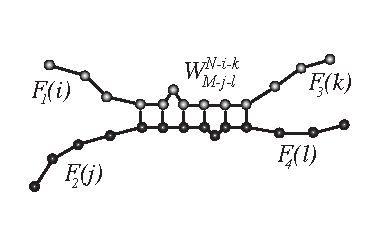
\includegraphics[width=\halffigure]{\FIGPATH/Figures_Partitionsum/partition}
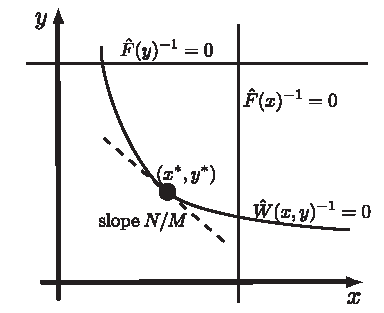
\includegraphics[width=\halffigure]{\FIGPATH/Figures_Partitionsum/poles}
\caption[Calculating the partition sum.]{\label{fig:partition}Left: Every base-pairing configuration can be described by the length of the single stranded ends 1 to 4 and the part bounded by base pairs.
Right: A sketch of the singularities of $\Fh(x)$, $\Fh(y)$ and $\Wh(x,y)$ in the positive quarter plane
of real $x$ and $y$. }
\end{figure}
The partition sum of the molecule with $N$ 
repeat units on one and $M$ repeat units on the other strand is thus given by
\begin{equation}
\label{eq:completeZ}
  Z(N,M)=\sum_{i,j,k,l=0}^{i+k< N, j+l< M}F_1(i)F_2(j)F_3(k)F_4(l)W_{M-j-l}^{N-i-k},
\end{equation}
where $F_i(n)$ are the statistical weights of the single stranded ends of length $n$ and $W_s^{r}$ is the sum of all possible configuration of a double stranded part with $r$ bases on one and $s$ bases on the other strand.
Similarly to the case where only native base pairs are allowed (see \SEC{DNA_melting}), $W_s^{r}$ can 
be calculated from the recursion relation
\begin{equation}
\label{eq:recursion}
  W_{s+1}^{r+1}=q_{s+1}^{r+1}W_{s}^r+q_{s+1}^{r+1}\sum_{k+m>1}^{k<r,m<s} \El(k,m)W_{s-m}^{r-k},
\end{equation}
where $q_{s}^{r}$ is the Boltzmann factor of the binding energy of base $r$ and base $s$ and $\El(k,m)$ is the cost 
of having a loop with $k$ bases on one and $m$ bases on the other strand. The first term of the
recursion relation accounts for all configuration where the base pair $(r+1,s+1)$ is added to 
any configuration in $W_{s}^r$, whereas the second term includes all configuration where the
base pair $(r+1,s+1)$ followed by a loop of size $(k,m)$ is added to any configuration in $W_{s-m}^{r-k}$.
One easily convinces oneself, that this recursion indeed generates all allowed configurations.

This recursion relation can be solved numerically for arbitrary sequences in $\mathcal{O}(N^{2}M^{2})$
operations \cite{Garel_Biopolymers_04, Bundschuh_PRE_02}. 
An analytical solution can be obtained, if the sequence is homogenous, that is  $q_{s}^{r}=q$,
and if $\El(k,m)$ is sufficiently well behaved. Note that every repetitive sequence is essentially homogeneous
since each repeat unit can be treated a single base which only binds to its native binding partner.
Again, the recursion relation can be solved by $z$-transformation, but this time different fugacities $x$ and $y$ 
for the two strands are needed since they can be of different length and are not necessarily in register. 
To this end, we multiply both sides by $x^{r}y^{s}$ and sum over $r$ and $s$ to obtain
\begin{equation}
\label{eq:recursion}
  \frac{\Wh(x,y)-xyW_1^{1}}{xy}=q\Wh(x,y)+q\Elh(x,y)\Wh(x,y),
\end{equation}
where $\Wh(x,y)=\sum_{r,s=1}^{\infty} W_s^{r}x^{r}y^{s}$, $\Elh(x,y)=\sum_{r,s=1}^{\infty} \El(r,s)x^{r}y^{s}$ and
$W_1^{i}=W_i^{1}=0$ for all $i>1$. This is readily solved for $\Wh(x,y)$, yielding
\begin{equation}
\label{eq:What}
 \Wh(x,y) = \frac{W_1^{1}}{\frac{1}{xy}-q-q\Elh(x,y)},
\end{equation}
The $z$-transform of the partition sum in \EQ{completeZ} is computed similarly and given by 
\begin{equation}
\label{eq:completeZ}
  \Zh(x,y)=\Fh_1(x)\Fh_2(y)\Fh_3(x)\Fh_4(y)\Wh(x,y),
\end{equation}
where $\Fh_i(z)$ is the one variable $z$-transform of the single stranded ends. 

The $z$-transformations in the base indices on both strands are equivalent to changing from a statistical 
ensemble with constant particle numbers to a grand ensemble, where the particle number is determined
by the fugacities of a particle reservoir. The grand partition sum is a power series in $x^{N}y^{M}$ with 
coefficients $Z(N,M)$. Therefore $Z(N,M)$ can in principle be obtained from $\Zh(x,y)$ by double contour integration
\begin{equation}
\label{eq:contour_int}
   Z(N,M)=-\frac{1}{4\pi^{2}}\oint\oint dxdy\;\frac{\Zh(x,y)}{x^{N+1}y^{M+1}}.
\end{equation}
In many cases, one of the integrals can be calculated by suitable deformation of the integration contour, but the
remaining integral is usually infeasible. Nevertheless, a great deal of information can be obtained from the 
function $\Zh(x,y)$, at least in the thermodynamic limit, which for linear molecules corresponds to the 
limit of long strands \cite{Tamm_PRE_07}. In this limit relative strand length fluctuations vanish and the grand ensemble is equivalent to the fixed length ensemble. The expected numbers of particles on both strands are given by 
\begin{equation}
\label{eq:mean_length}
\begin{split}
  \langle N \rangle= x\frac{\partial \ln\Zh(x,y)}{\partial x}\quad \mathrm{and}\quad
   \langle M \rangle= y\frac{\partial \ln\Zh(x,y)}{\partial y},
\end{split}
\end{equation}
and for $\langle N \rangle$ or $\langle M \rangle$ to become arbitrarily large, $\Zh(x,y)$ has to diverge. 
The thermodynamic limit
thus confines the set of possible fugacities to the singularities of $\Zh(x,y)$, which in general 
form a one dimensional, possibly multiply branched, set (cf.~right part of \FIG{partition}). 
To fix the fugacities completely, we need an additional condition. 
This is given by the requirement, that the ratio of the two strand length remains constant
as the thermodynamic limit is approaches. Otherwise, the intensive properties of the system 
are not preserved. We thus have to choose the fugacities $(\xf, \yf)$ such that
\begin{eqnarray}
\label{eq:partsum_divergence}
 \nonumber
  &\lim_{x,y\rightarrow \xf,\yf}\langle N \rangle= \infty \qquad \mathrm{and}\qquad \lim_{x,y\rightarrow \xf,\yf}\langle M \rangle= \infty\\
&\lim_{x,y\rightarrow \xf,\yf}\frac{\langle N \rangle}{\langle M \rangle}=c. 
\end{eqnarray}
Since the free energy of the DNA molecule should be extensive, the partition sum for long strands of 
length $N$ and $cN$ is of the form $Z(N, cN )= \gamma^{N}$.
From the definition $\Zh(x,y)=\sum_{N,M=1}^{\infty} Z(N,M)x^{N}y^{M}$ and the fact that only 
configurations with $M\approx Nc$ contribute, we have 
$\Zh(x,y)\sim(1-\gamma^{N}x^{N}y^{cM})^{-1}$. Hence, the singularities of $\Zh(x,y)$ lie on the curve 
$\xf\yf^{c}=\gamma^{-1}$. The limit of infinite strand length is approached from below $|xy^{c}|<\gamma^{-1}$. 
Within this approximation, which essentially is a saddle point approximation, the free energy of a 
molecule out of strands of length $N$ and $M$ is given by 
\begin{equation}
\label{eq:free_energy}
   F(N,M)=-\kT\ln Z(N,M) = N \ln \xf + M \ln \yf,
\end{equation}
where the free energies per base $\ln \xf$ and $\ln \yf$ are determined by \EQ{partsum_divergence} and 
\EQ{mean_length}. Alternatively, one can perform the inverse transformation in one variable and thereby 
fix one strand length and then determine the remaining fugacity such that the expected length of the 
other strands matches the desired value. We will now apply this formalism to concrete problems of
repetitive DNA under shear force and thermal denaturation of DNA. 
A more detailed description of this derivation is given in \REF{Tamm_PRE_07}.
 
\section{Thermal denaturation of repetitive DNA}
To describe the melting transition of repetitive DNA, we have to specify the Boltzmann factor associated with
the binding of one repeat unit and the statistical weights of loops and single stranded ends. 
The statistical weights of loops and free ends are dominated by the entropy of the different 
configurations available to the flexible polymer, as already discussed in \SEC{DNA_melting}. 
The statistical weights of free single stranded ends of length $n$ and of loops with $n$ and $m$
on the two strands are given by
\begin{equation}
F(n)=\frac{s^n}{n^{\bar{c}}} \qquad \mathrm{and} \qquad \El(n,m)=g^{2}\frac{s^{n+m}}{(n+m)^c},
\end{equation}
where the exponents $\bar{c}$ and $c$ describe the excluded volume effects of an open end and 
a closed loop. While $\bar{c}$ is irrelevant for the melting transition, $c$ is pivotal and its value is assumed 
to lie in the range $1.8\ldots2.15$ \cite{Kafri_PRL_00} (cf.~\SEC{DNA_melting}). 
The $z$ transformations of the weights are given by
\begin{equation}
\Fh(x)=\Phi_{\bar{c}}(xs) \qquad \mathrm{and} \qquad \Elh(x,y)=g^{2}\frac{x\Phi_c(xs)-y\Phi_c(ys)}{x-y}.
\end{equation}
The factor $g^{2}$ accounts for a finite energy penalty to initiate a loop. The function $\Phi_c(z)$
is the polylogarithm, which is analytic everywhere in the complex plane, except on the interval
$[1,\infty[$ of the real axis. 

Inserting $\Fh(x)$ and $\Elh(x,y)$ into equation \EQ{completeZ} yields the grand canonical 
partition sum two homogeneous DNA strands. As described above, the asymptotic behavior of 
the two strands is governed by the singularity of $\Zh(x,y)$ which is closest to the origin, subject to the
constraint that the ratio of the two strand length is fixed. 
Depending on whether this singularity is the branch-cut induced by the polylogarithm 
or an isolated singularity of  $\Wh(x,y)$, the two strands are denatured or bound to each other. 
The phase behavior of such systems is discussed in \SEC{intermediate_phase}.

\section{Pulling on repetitive DNA}
When exerting a shear force to the DNA, we have to distinguish between ends where the 
force is applied to and the unstretched ends. From now on, we model the ssDNA by the freely jointed 
chain (FJC) model, neglecting self-avoidance. Furthermore, we give all energies relative 
to unconstrained single strand. Consequently, for unstretched ends we have $F_{2}(n)=1$
 irrespective of the length $n$. The transformed $\Fh_{2}(x)$ is given by $(1-x)^{{-1}}$. 
 The free energy of the DNA molecule in the external force field is given by the product
 of an effective length $L$ and the magnitude of the force. This effective length can be calculated
 separately for the single stranded ends and the double stranded region in between.  
The free energy of a segment of a FJC polymer with Kuhn length $l_k$ under a tension 
 $f$ is given by the integral over all orientations of a segment
\begin{equation}
\frac{1}{2}\int e^{-\frac{fl_k\cos \theta}{\kT}}\sin \theta d\theta=\frac{\kT}{fl_k}\sinh\left(\frac{fl_k}{\kT}\right).
\end{equation}
The free energy per monomer of length $\lss$ is thus given by 
$f\cdot\tss=\frac{\lss}{l_k}\ln\left(\frac{\kT}{fl_k}\sinh\left(\frac{fl_k}{\kT}\right)\right)$, 
where $\tss$ is an effective length. The contribution of stretched ssDNA of length $n$ is 
therefore $F_{1}(n,f)=e^{n \tss f}=\ebs^n$ and its $z$-transform reads $\Fh_{1}(x,f)=(1-x\ebs)^{-1}$.
dsDNA is sufficiently stiff and long, such that we can assume that its completely aligned, yielding 
a free energy per base pair $f\cdot\lds$.  Together with the binding free energy the statistical weight
of a base pair is given by $q=e^{f\lds+\eps}=\ebd q_0$. 
The statistical weights of loops within the sequence is a bit more subtle to calculate. We assume, 
that the projected length of a loop is given by the length the shorter arm would have when in a double
helix. As loop cost function, we use  $\El(n,m,f)=g^{2}e^{\lds\min(n,m)f}=g^{2}\ebd^{\min(n,m)}$, where $g^{2}$ accounts for loop initiation and the exponential for the stretching energy. 
The two variable $z$-transformation of this quantity is a bit laborious and yields
\begin{equation}
\Elh(x,y,f)=\frac{g^2}{1-\ebd xy}\left(\frac{x}{1-x}+\frac{y}{1-y}+\ebd\right)
\end{equation}
Inserting the different functions for loop cost and single strand contributions in \EQ{completeZ}
yields the grand canonical partition sum for sheared DNA. The single strand factors have obvious
singularities at $x=1$, $y=1$, $x=\ebs^{-1}$ and $y=\eps^{-1}$, corresponding to no stable binding 
 and completely stretched single strand, respectively. At low forces, however, $\Wh(x,y)$ has
an additional singularity at $(\xf, \yf)$ corresponding to a state where the two strands bind with maximal 
overlap. The transition from this bound state the stretched state occurs when $(\xf,\yf) = (\ebs^{-1}, \ebs^{-1})$.
In the limit of high loop cost the contribution $\Elh(x,y,f)$ in the denominator can be neglected and 
it is easily seen that the singularity is found at $\xf\yf=\ebd q_0$. The transition to the open state
occurs at $\xf\yf=\ebs^{-2}=\ebd q_0$, which is yields $\fc=\frac{\eps}{2\tss-\lds}$. At finite loop
cost the double stranded region is stabilized by the combinatorial entropy of the different double stranded
conformations. Typically, this contribution is small.


\subsection{Determining loop densities.}
In \SEC{DNA_sliding}, it was argued that the sliding velocities can be calculated from the 
pseudo-equilibrium loop densities, which in turn can be calculated from the proper equilibrium 
properties of a suitably chosen system. This system cannot be a double
strand with a shear force applied, since at equilibrium in the supercritical regime, there is no double stranded
region and no loop density can be defined. The argument leading to the pseudo-equilibirium density 
was, that the two strands move slowly relative to each other, such that the densities at the ends 
equilibrate. We now idealize this assumption, by attaching both strands to a wall at one end, and apply
a force to the longer strand at the other end, at illustrated in \FIG{loop_densities}.
\begin{figure}
\centering
\includegraphics[width=\smallfigure]{\FIGPATH/Figures_Partitionsum/loopdensities}
\caption[Calculating loop densities.]{\label{fig:loop_densities} Using a double strand attached to a wall, we can 
calculate the loop densities on the stretched and unstretched strands, even for $f>\fc$.}
\end{figure}
The partition sum of this system is given by 
\begin{equation}
\label{eq:Z_fdenat}
  \Zh(x,y)=\Fh_s(x)\Fh_u(y)\Wh(x,y),
\end{equation}
where the stretched single strand contributes $\Fh_s(x)=(1-x\ebs^{{-1}})$, the unstretched single strand
$\Fh_u(y)=(1-y)^{-1}$ and $\Wh(x,y)$ is the same as above. Given the complete partition sum, we can now
calculate the average number of base pairs via
\begin{equation}
	\langle N_{bp}\rangle=\frac{\partial \ln \Zh(x,y)}{\partial \ln q}.
\end{equation}
Furthermore, we can calculate the number of nucleotides on the upper and lower strand inside the 
double helical region by 
\begin{equation}
	\langle N_{u}\rangle=\frac{\partial \ln \Wh(x,y)}{\partial \ln x} \qquad \mathrm{and} \qquad
	\langle N_{l}\rangle=\frac{\partial \ln \Wh(x,y)}{\partial \ln y}.
\end{equation}
Similarily, we can calculate the average number of loops inside the double helical region by differentiating
$\ln \Zh(x,y)$ with respect to $2\ln g$. From these quantities the loop densities, the stored length and 
the mean loop size are readily calculated. 




  \chapter{\label{app:genLanger}Generalized Kramers-Langer rates}
This appendix provides a detailed derivation of the generalized Kramers-Langer-Theory presented
in \SEC{tsr}. The derivation is kept general and we refer the reader to \SEC{tsr} or the publication reprinted
in \SEC{tsr_rotor} for a concrete application. In 1969, J.~Langer published a generalization of the celebrated
Kramers' formula for thermally activated escape from a one-dimensional potential well to barrier 
crossing processes in many dimensions \cite{Langer_APNY_69}. 
A concise and clear derivation of this formula can be found in \REF{Haenggi_RevModPhys_90}.
The Langer formula, as presented by \citeauthor{Haenggi_RevModPhys_90}\cite{Haenggi_RevModPhys_90}, assumes a constant
mobility matrix in the relevant saddle point region. However, in many systems and especially in those described by
generalized coordinates, this assumption cannot be made. 
Here, we seek to incorporate the configuration dependence of the mobility matrix into the Langer formula. 

The escape rate out of a meta-stable potential well separated from a stable region by a unique
saddle point is given by ratio of the probability current over the saddle point and the population 
inside the well. The evolution of the probability density $\PD(\{\eta\})$ is determined by the 
Fokker-Plank equation (FPE) $\partial_t \PD(\{\eta\},t)=-\nabla\cdot\mathbf{j}(\{\eta\},t)$, where the
flux density $\mathbf{j}(\{\eta\},t)$ is given by
\begin{equation}
\label{eq:FPE}
%\frac{\partial \PD(\{\eta\})}{\partial t} = \partial_i \left[\Mobc_{ij}\frac{\partial U(\{\eta\})}{\partial \PD_j}+\kT\Mobc_{ij} \partial_j \right]\PD(\{\eta\}),
j_i (\{\eta\},t)= -\left[\Mobc_{ij}\frac{\partial V(\{\eta\})}{\partial \eta_j}+\kT\Mobc_{ij} \partial_j \right]\PD(\{\eta\},t),
\end{equation}
The matrix $\Mob$ is the mobility matrix which in general depends on the configuration 
$\{\eta\}$ and $V(\{\eta\})$ is the potential energy.
We consider only the purely diffusive case and neglect any symplectic contributions to $\Mob$, 
which is justified since the applications in mind are completely overdamped.
Let us now assume that particles are injected into the meta-stable well at a constant rate and removed
from the stable region. In this case, $\PD(\{\eta\})$ tends to a steady state, with a distribution that is very close
the equilibrium distribution inside the meta-stable well, and which vanishes beyond the saddle where particles are
removed. This steady state distribution carries a probability flux density out of the meta-stable well into the
region where particles are removed. Obviously, the total flux integrated over any surface separating the insertion site from the absorbing boundary is equal to the rate of particle insertion. The non-trivial task 
is to relate this flux to the population inside the meta-stable well, \emph{i.e}~the number of 
particles that accumulate before the steady state is attained. To this end, we solve the FPE in the vicinity
of the saddle point where the probability flux is concentrated to a narrow channel, and
match this solution to the approximate pseudo-equilibrium solution inside the meta-stable region.
%The mobility matrix relates the forces and the spatial inhomogeneities to the the probability flux.
The size of the relevant saddle point region is determined by the curvature of the potential 
energy at the saddle point. Within this region, we can expand the potential 
energy, resulting in the simple FPE
\begin{equation}
\label{eq:steadyFPE}
\partial_i \left[\Mobc_{ij}\UHessc_{jk}\eta_k+\Mobc_{ij}\kT \partial_j \right]\PD(\{\eta\}) =0,
\end{equation}
where $\UHess$ is the Hessian of the energy near the saddle point.
Since we need to match the solution near the saddle point to the equilibrium distribution inside the well,
we rewrite $\PD(\{\eta\})$ in the form 
$\PD(\{\eta\})=\PD_{eq}(\{\eta\})\Ansatz(\{\eta\})$, where $\PD_{eq}(\{\eta\})$ is the equilibrium distribution. 
Using this ansatz we can decompose the above equation into the equations
\begin{equation}
\begin{split}
\label{eq:flux}
\partial_i \Ansatz(\{\eta\}) \left[\Mobc_{ij}\UHessc_{jk}\eta_k+\kT \Mobc_{ij}\partial_j \right]\PD_{eq}(\{\eta\})=0\\
\partial_i \PD_{eq}(\{\eta\})\kT \Mobc_{ij} \partial_j \Ansatz(\{\eta\})=0,
\end{split}
\end{equation}
the first of which is trivially fulfilled since it includes the current of $\PD_{eq}(\{\eta\})$. 

If the mobility matrix changes significantly inside the saddle point region, its variation has to be taken into account. 
Here, we seek to incorporate this variations by expanding the mobility matrix about the saddle point
and calculate the correction to the rate. 
%To calculate this flux, we expand the 
%the potential landscape and the mobility matrix around the saddle point and solve the FPE
%in a harmonic approximation for a steady state solution. It has to be taken care that the expansion of the
%mobility matrix is reasonable inside the relevant saddle point region and in particular does not become negative.
Each entry of the mobility matrix $\Mob$ can be expanded separately as
\begin{equation}
\Mobc_{ij}=\Mobc_{ij}^0+\frac{\partial \Mobc_{ij}}{\partial \eta_k}\eta_k + \frac{1}{2}\frac{\partial^2 \Mobc_{ij}}{\partial \eta_k\partial \eta_l}\eta_k\eta_l+\mathcal{O}(\eta^2),
\end{equation}
where $\eta_k$ are the deviations from the saddle.
For symmetry reasons the linear dependence on $\eta_k$ will often vanish and for the moment we will drop 
the linear term. In short, we have 
$\Mobc_{ij}=\Mobc_{ij}^0+\frac{1}{2}\MobHessc_{kl}^{ij}\eta_k\eta_l$
with the symmetric matrix $\mathbf{A}^{ij}$ for each entry of $\Mob$. 
Inserting this expansion into \EQ{flux} yields
\begin{equation}
\begin{split}
\label{eq:flux_ansatz}
\left[-\UHessc_{ik}\Mobc_{ij} + \kT \NIDcoeff_{jk}\right]\eta_k\partial_j \Ansatz(\{\eta\})+
\kT \Mobc_{ij} \partial_i \partial_j \Ansatz(\{\eta\})=0\;,
\end{split}
\end{equation}
where the matrix $\NID$ is defined by 
\begin{equation}
\partial_i \Mobc_{ij}= \frac{1}{2}\sum_{i} \left(\delta_{il}\MobHessc_{lk}^{ij}\eta_k+\delta_{ik}\MobHessc_{lk}^{ij}\eta_l\right)=\sum_{i}\MobHessc_{ik}^{ij}\eta_k=\NIDcoeff_{jk}\eta_k.
\end{equation}
$\NIDcoeff_{kl} \eta_l$ is the noise induced drift due to the configuration dependence of the 
mobility matrix and which is absent in the conventional Langer theory. 
To solve this equation, we employ the ansatz \cite{Haenggi_RevModPhys_90}
\begin{equation}
\Ansatz(\{\eta\})=\frac{1}{\sqrt{2\pi\kT}}\int_u^{\infty}\exp(-\frac{z^2}{2\kT}) dz,
\end{equation}
where the lower integration boundary depends on $\eta_k$ via $u=\sum_i \Sepc_i\eta_i$, where the 
vector $\Sep$ is to be determined by \EQ{flux_ansatz}.
This function interpolates smoothly between one inside the meta-stable region and
tends to zero beyond the saddle point and therefore automatically satisfies the matching condition.
Inserting this ansatz into \EQ{flux_ansatz} yields, after a bit of algebra
\begin{equation}
\label{eq:eigenvectoreq}
\begin{split}
\left[\Sepc_j(-\Mobc_{ji}\UHessc_{ik}  + \kT \NIDcoeff_{jk}) -
\Sepc_i \Mobc_{ij} \Sepc_j\Sepc_k\right]\eta_k=0
\end{split}
\end{equation}
Since this equation should hold for any set $\eta_k$, the term in brackets itself has to vanish.
%\begin{equation}
%\label{eq:eigenvectoreq}
%\begin{split}
%(-\Mobc_{ji}\UHessc_{ik} + \kT \NIDcoeff_{jk}) \Sepc_j-(\Sepc_i\Mobc_{ij} \Sepc_j)\Sepc_k=0
%\end{split}
%\end{equation}
\EQ{eigenvectoreq} is equivalent to equation 4.71 in \REF{Haenggi_RevModPhys_90}, but includes the 
additional drift $\kT \NIDcoeff_{jk}\eta_k$ induced by the configuration dependence of $\Mob$. In this equation,
the explicit configuration dependence of $\Mobc_{ij}=\Mobc_{ij}^{0}+\frac{1}{2}\MobHessc_{kl}^{ij}\eta_k\eta_l$
is of second order in $\eta_k$ and can therefore be neglected. After substituting $\Mobc_{ij}^{0}$
for $\Mobc_{ij}$, \EQ{eigenvectoreq} is an eigenvector equation 
for $\Sep$, which determines $\Sep$ to be a left eigenvector of $-\Mobc_{ji}^0\UHessc_{ik}  + \kT \NIDcoeff_{jk}$. 
The norm of $\Sep$ is fixed by the condition $\lambda=\Sepc_i\Mobc_{ij}^0 \Sepc_j$, where $\lambda$ is the
eigenvalue corresponding to the eigenvector $\Sep$. In particular, this condition requires $\lambda$ 
to be positive. The necessity of the noise-induced drift term is illustrated in \FIG{separatrix}, where the stochastic separatrix is 
plotted for different temperatures. The vector $\Sep$ has an appealing interpretation:
$\Sep$ is perpendicular to the stochastic separatrix, \emph{i.e.}~the hyperplane where the probabilities
to relax either into the meta-stable or stable region are both equal to 0.5. The right eigenvector to the same eigenvalue
points into the direction of the diffusive flux at the transition state \cite{Berezhkovskii_JChemPhys_05}. The right 
and left eigenvectors coincide if $\Mob$ is diagonal.
%If the $\NIDcoeff_{jk}$ vanish, the latter implies 
%$\Sep e^{-1}_{ij}\Sepc_j=-\frac{1}{\lambda}\Sepc_l \Mobc_{lk}\UHessc_{ki}e^{-1}_{ij}\Sepc_j=-1$.
%For non zero $\NIDcoeff_{jk}$, one has $\Sepc_i e^{-1}_{ij}\Sepc_j=-1 + \frac{kT}{\lambda}\Sepc_l \NIDcoeff_{li}e^{-1}_{ij}\Sepc_j$.
%This correction term will reappear later on.
\begin{figure}
\centering
\includegraphics[width=\halffigure]{\FIGPATH/Figures_AppendixB/separatrix}
\caption[The effect of noise-induced drift on the stochastic separatrix.]
{\label{fig:separatrix} The slope of stochastic separatrices at the saddle point changes with temperature. The slope 
calculated from the left eigenvector of $-\Mobc_{ji}^0\UHessc_{ik}  + \kT \NIDcoeff_{jk}$ (solid lines) agrees with simulation results (symbols) within their uncertainty.}
\end{figure}


\section{The flux over the barrier}
Given the approximate steady state solution of the FPE, the probability flux reads
\begin{equation}
j_i=-\left[\Mobc_{ij}\frac{\partial V(\{\eta\})}{\partial \eta_j}+\kT\Mobc_{ij} \partial_j \right]\PD(\{\eta\})=\frac{\kT \PD_{eq}(\{\eta\})}{\sqrt{2\pi\kT}}\exp(-\frac{u^2}{2\kT}) \,\Mobc_{ij} \Sepc_j,
\end{equation}
where $\Mobc_{ij}$ is the full configuration dependent mobility matrix. The total flux out of the 
meta-stable region can now be calculated by integrating the flux density over a surface
surrounding that region. To calculate the total flux over the saddle, we integrate the flux density over
the plane given by the separatrix $u=0$\footnote{Any plane that separates the meta-stable well from
the absorbing boundary can be used, the separatrix is a particularly convenient choice.} (cf.~Appendix of \REF{Haenggi_RevModPhys_90}). Since the flux is strongly concentrated at the saddle point, 
we can again expand the potential energy and the mobility matrix. The resulting integral reads
\begin{equation}
J=Z^{-1}\sqrt{\frac{\kT}{2\pi}}\int_{u=0}\frac{ds}{|\Sep|} \;e^{-\frac{1}{2}\frac{\UHessc_{ij}\eta_i\eta_j}{\kT}}\Sepc_i\left(\Mobc^0_{ij}+\frac{1}{2}\MobHessc^{ij}_{kl}\eta_k\eta_l\right) \Sepc_j\:,
\end{equation}
where $\PD_{eq}(\{\eta\})=Z^{-1}e^{-\frac{1}{2}\frac{\UHessc_{ij}\eta_i\eta_j}{\kT}}$ was substituted for the equilibrium 
distribution.
To facilitate the evaluation of this surface integral it is helpful to choose suitable coordinate system. 
Let the direction of the first coordinate coincide with the vector $\Sep$, which is then obviously of the form $\Sepc_i=\delta_{i1} \Sepc_1$.
In this particular system of coordinates, the surface integral reduces to the integral
over the coordinates $2, \ldots, N$, with $\eta_1=0$. 
\begin{equation}
\label{eq:totalflux}
J=Z^{-1}\sqrt{\frac{\kT}{2\pi}}\int_{\eta_1=0} \prod_{l>1} d\eta_l\; e^{-\frac{1}{2}\frac{\UHessc_{ij}\eta_i\eta_j}{\kT}} \Sepc_1\left( \Mobc^{0}_{11}+\frac{1}{2}A^{11}_{ij}\eta_i\eta_j\right) 
\end{equation}
The integral over the first term in parenthesis is readily evaluated, yielding
\begin{equation}
\begin{split}
J^{0}=Z^{-1}\frac{\lambda}{\Sepc_{1}}\sqrt{\frac{\kT}{2\pi}}\frac{1}{|\redUHess^{11}/(2\pi\kT)|^{\frac{1}{2}}},
\end{split}
\end{equation}
where $\redUHess^{11}$ is the matrix $\UHess$ with the first column and row removed\footnote{The reduced matrix 
$\redUHess^{11}$ is positive definite and symmetric.}. The
normalization of $\Sep$ has been used to substitute $\frac{\lambda}{\Sepc_1}$ for $\Sepc_1\Mobc^{0}_{11}$.
The integral of the second term can be evaluated by choosing the remaining coordinates such that 
$\redUHess^{11}$ is diagonal. 
\begin{equation}
\begin{split}
J^{corr}&=Z^{-1}\sqrt{\frac{\kT}{2\pi}}\int_{\eta_1=0} \prod_{l>1} d\eta_l \;\Sepc_1\frac{1}{2}A^{11}_{ij}\eta_i\eta_j e^{-\frac{1}{2}\UHessc_{ij}\eta_i\eta_j}\\
&=Z^{-1}\sqrt{\frac{\kT}{2\pi}} \frac{\Sepc_1}{2|\redUHess^{11}/(2\pi\kT)|^{\frac{1}{2}}}\sum_{l>1} \frac{\MobHessc^{11}_{ll}}{\hat{\mu}_l}\end{split}
\end{equation}
where the diagonal elements of the reduced matrix $\redUHess^{11}$ are denoted by $\hat{\mu}_2, \ldots, \hat{\mu}_N$.
To express the determinant of $\redUHess^{11}$ in the denominator through the determinant of the full 
Hessian of the potential energy, we need the relation
\begin{equation}
\Sepc_i \UHessc^{-1}_{ij}\Sepc_j=\frac{1}{\lambda}\Sepc_l (-\Mobc^{0}_{lk}\UHessc_{ki}+\kT \NIDcoeff_{li})\UHessc^{-1}_{ij}\Sepc_j=-1 + \frac{\kT}{\lambda}\Sepc_l \NIDcoeff_{li}e^{-1}_{ij}\Sepc_j=-1+\NIDcorr,
\end{equation}
where $\NIDcorr$ is a solely due to the noise induced drift.  Using the well known formula 
for inverse matrices  $\UHessc^{-1}_{kl}=\frac{1}{|\UHess|} (-1)^{k+l}|\redUHess^{kl}|$, we have
$|\redUHess^{11}|=|\UHess|\UHessc^{-1}_{11}=|\UHess|=-|\UHess|\frac{1-\NIDcorr}{\Sepc_1^{2}}$.
Putting everything together, we find for the total flux out of the meta-stable well
\begin{equation}
\begin{split}
J=Z^{-1}\frac{\lambda}{2\pi}\frac{1}{|\UHess/(2\pi\kT)|^{\frac{1}{2}}(1-\NIDcorr)^{\frac{1}{2}}}\left(1+\frac{1}{2 \Mobc_{11}}\sum_{l>1} \frac{A^{11}_{ll}}{\hat{\mu}_l}\right),
\end{split}
\end{equation}
The population inside the meta-stable region can be calculated within a Gaussian approximation
\begin{equation}
\begin{split}
\label{eq:pop_in_meta}
N %&=\int d\eta \PD(\{\eta\})=\int d\eta \PD_{eq}(\{\eta\})\Ansatz(\{\eta\})\\
&=Z^{-1}\int d\eta e^{-\frac{\frac{1}{2}\UHessc^{w}_{ij}\eta_i\eta_j-\dU}{\kT}}
=\frac{e^{\frac{\dU}{\kT}}}{Z|\UHess^{w}/(2\pi\kT)|^{\frac{1}{2}}}\;,
\end{split}
\end{equation}
where $\UHess^{w}$ is the Hessian of the potential energy at the bottom of the meta-stable potential 
well. Dividing the flux by the population inside the meta-stable well yields the generalized Langer 
rate  
\begin{equation}
\label{eq:genLangerrate}
k=\frac{J}{N}=\frac{\lambda}{2\pi}
\sqrt{\frac{|\UHess^{w}|}{|\UHess^{t}|(1-\NIDcorr)}}e^{-\frac{\dU}{\kT}}
\left(1+\frac{1}{2 \Mobc_{11}}\sum_{l>1} \frac{A^{11}_{ll}}{\hat{\mu}_l}\right),
\end{equation}
where we labeled the the Hessian at the transition state with a superscript $t$.  
The different terms of this rate are easily interpreted. The ratio of the determinants, the exponential
factor and the correction due to noise induced drift are the probability of finding the system near 
the transition state. The eigenvalue $\lambda$ is the relaxation rate from the saddle.
The term in parenthesis quantifies by what amount the mobility of the reaction coordinate
averaged over the relevant window surrounding the saddle differs from the mobility at the saddle point itself.
Note, that the latter correction term is given in the coordinate system where $\eta_1$ coincides with the
direction of the reaction coordinate. 


\section{Stochastic dynamics of constrained systems}
Many microscopic systems such as polymer chains or proteins have some degrees of freedom 
that vary in a large range and others that are confined to a very narrow range. Typically, the former are
bending angles while the latter are linear dimensions. It is therefore tempting
to replace the strongly confined degrees of freedom by rigid constraints and describe the
system with generalized coordinates corresponding to the large amplitude degrees of freedom. 
Such a natural choice of coordinates is often helpful to elucidate the essential features of the 
system. Eliminating strongly confined degrees of freedom has also practical 
advantages, since the steep confining potentials require very small simulation time steps.
Unfortunately, the limiting procedure to eliminate the constrained coordinates is ambiguous and
the subtle difficulties arise where none would be expected. Quite generally, intuition is not a very
good guideline when it comes to stochastic dynamics is curvilinear coordinate systems and things
go awfully wrong if insufficient care is taken. 
These difficulties not only affect the dynamics of the system, but also the equilibrium distribution
of the spatial coordinates. To illustrate this, let us consider a system with constrained and 
unconstrained degrees of freedom and compare their equilibrium distribution using rigid or 
flexible constraints. The Hamiltonian of the rigid version is given by 
\begin{equation}
H(\{p_i\},\{q_i\})= \frac{1}{2} p_k t_{kl}(\{q_i\})p_l+V(\{q_i\}), 
\end{equation}
where $\{q_i\}$ are the generalized coordinates, $\{p_i\}$ are the conjugate momenta,  
$t_{kl}(\{q_i\})$ is the quadratic form of the kinetic energy\footnote{
$t_{kl}(\{q_i\})$ is the inverse of the mass matrix in generalized coordinates.},
and $V(\{q_i\})$ is the potential energy of the unconstrained coordinates. 
The corresponding energy function for the system with flexible constraints 
 in cartesian coordinates is
\begin{equation}
H(\{\dot{x}_i\},\{x_i\})= \sum_i \frac{m_i}{2} \dot{x}_i^{2}+V(\{q_i(\{x_i\})\})+U(\{x_i\}), 
\end{equation}
where $m_i$ are the masses and $U(\{x_i\})$ is the confining potential for the stiff directions.
Submerged in a heat bath, the equilibrium distribution of the $\{q_i\}$ and their conjugate momenta
$\{p_i\}$ is the Boltzmann distribution. The same holds true for the cartesian coordinates. However, 
after integrating over $\{p_i\}$, the distribution of the $\{q_i\}$ alone is no longer of Boltzmann form, but reads
\begin{equation}
\PD_{rigid}(\{q_i\})\sim \frac{1}{|t_{kl}(\{q_i\})|^{\frac{1}{2}}} e^{-\frac{V(\{q_i\})}{\kT}}
\end{equation}
Integrating over momenta in cartesian coordinates is trivial. To compare the distribution of the spatial
coordinates in both systems, lets express the cartesian coordinates by the unconstrained coordinates $\{q_i\}$ and the 
coordinates along the constraints $\{r_i\}$. Integrating over the $\{r_i\}$ yields
\begin{equation}
\PD_{flex}(\{q_i\}) \sim g(\{q_i\}) e^{-\frac{V(\{q_i\})}{\kT}},
\end{equation}
where $g(\{q_i\})$ is the left-over of  the Jacobian determinant of the coordinate 
transformation. Even for very simple systems, $\PD_{flex}(\{q_i\})$ and $\PD_{rigid}(\{q_i\})$ are different 
\cite{Helfand_JChemPhys_79, vanKampen_AJP_84, Fixman_PNAS_74}, although the potential energies are the same. 
When introducing the confining potential $U(\{x_i\})$ we assigned a small range to each constrained coordinate, which is independent of the $\{q_i\}$. We then integrated over constrained momenta
and coordinates, resulting in a distribution that does not favor any region of the space of $\{q_i\}$'s apart
from the volume element of the $\{q_i\}$-coordinate system. When using rigid constraints, we ignore momenta of the 
constrained direction from the start. The integration over the conjugate momenta reduces the complete
phase space to a subspace where some regions are favored over others. 
Loosely speaking, in these regions the conjugates momenta have a 
greater number of states available than in other regions.

We are interested in the stochastic dynamics of constrained systems, but we want to interpret them as
stiff limits of physical springs since there are no truly rigid constraints in classical physics. If even the 
equilibrium properties of constrained systems are ambiguous or incompatible with the physical picture,
dynamical features certainly are too.
In the case of overdamped dynamics, however, there is a remedy to this problem. The 
difference between stiff and rigid constraints can 
be compensated by a pseudo potential \cite{Helfand_JChemPhys_79, Fixman_JChemPhys_78a, Roitman_JChemPhys_84}.
Here, we apply a somewhat reverse, but equivalent strategy. We 
impose an equilibrium distribution on the generalized spatial coordinates $\{q_{i}\}$ of the form 
\begin{equation}
\label{eq:Peq}
\PD_{eq}(\{q_i\}) \sim e^{-\Omega(\{q_i\})} e^{-\frac{V(\{q_i\})}{\kT}},
\end{equation}
where $V(\{q_i\})$ is the potential energy of the system and $\Omega(\{q_i\})$ accounts for
obvious dependencies of the volume element on the $\{q_i\}$, \emph{e.g.}~$\Omega(\theta)=-\ln(\sin \theta)$ for
three dimensional spherical coordinates. The key observation now is, that the choice of the equilibrium
 distribution and the deterministic overdamped relaxation fixes the 
Fokker-Planck equation governing the evolution of the probability distribution. 
The equations describing the deterministic relaxation of constrained
systems can be most conveniently obtained from the Euler-Lagrange equations including 
friction \cite{Goldstein}, which in the overdamped limit  simplify to 
\begin{equation}
\label{eq:lagrange}
\frac{\partial P(\{q_i\}, \{\dot{q}_i\})}{\partial \dot{q}_j}=-\frac{\partial V(\{q_i\})}{\partial q_j}.
\end{equation}
Assuming linear friction, the dissipation function $P(\{q_i\}, \{\dot{q}_i\})$ is given by the kinetic energy with all masses 
$m_{i}$ substituted by the particle mobilities $\mu_{i}$. 
Hence, $P(\{q_i\}, \{\dot{q}_i\})$ is a quadratic form in $\{q_i\}$ and equation \EQ{lagrange} 
can be solved for $\{\dot{q}_i\}$
\begin{equation}
\label{eq:det_eq}
\dot{q}_i=-\Mobc_{ij}(\{q_i\})\frac{\partial V(\{q_i\})}{\partial q_j},
\end{equation}
where $\Mob(\{q_i\})$ is the configuration dependent mobility matrix given by the inverse of the friction
matrix $\mathbf{P}(\{q_i\})$. The system obeys detailed balance, requiring that the net probability flux vanishes 
for $\PD_{eq}(\{q_i\})$
\begin{equation}
\label{eq:probFlux}
	j_k= \left[F_k +D_{kl} \frac{\partial }{\partial q_l} \right]\PD_{eq}(\{q_i\})=0.
\end{equation}
Here, the $F_k$ are general drift terms for each coordinate and $D_{kl}$ is the diffusion matrix. 
The  drift terms have to reduce to the deterministic relaxation
in the low temperature limit and can be written in the form $F_k=-\Mobc_{kl}\partial_l V(\{q_i\})+F_k^{noise}$.
$F_k^{noise}$ are stochastic drift terms absent in the low temperature limit. Since
the potential $V(\{q_i\})$ is arbitrary for a particular system with mobility matrix $\Mob$, 
the fluctuation dissipation theorem $D_{kl}=\kT \Mobc_{kl}$ follows immediately. This identification 
fixes the noise induced drift forces to $F_k^{noise}=-\kT \Mobc_{kl} \partial_l \Omega(\{q_i\})$, which 
vanishes at zero temperature as required.
The full Fokker-Plank equation of our system is therefore given by
\begin{equation}
\label{eq:ContrainedFPE}
\frac{\partial }{\partial t}\PD(\{q_i\},t)= \frac{\partial}{\partial q_k} \Mobc_{kl}(\{q_i\})
\left[ \partial_l V(\{q_i\})+\kT \partial_l \Omega(\{q_i\})+\kT\frac{\partial}{\partial q_l}\right] \PD(\{q_i\},t)
\end{equation}
From this Fokker-Plank equation, a simple procedure leads to the Langevin equations, which are to 
interpreted in the Ito sense \cite{Gardiner_04}. Since $\Mob$ is positive definite and symmetric, 
a matrix $\mathbf{B}$ with $\kT \Mobc_{ij}=B_{il}B_{jl}$ can be found, and the stochastic dynamics of the $q_i$
is governed by the equation
\begin{equation}
\label{eq:LangevinEQ}
\dot{q}_k=-M_{kl}(\{q_i\})\left[\partial_l V(\{q_i\})+\kT \partial_l \Omega(\{q_i\})\right]
+\kT\frac{\partial }{\partial q_l}M_{kl}(\{q_i\})+\sqrt{2}B_{kl}(\{q_i\})\eta_l,
\end{equation}
where $\eta_l$ is a vector of Gaussian white noise terms with unit variance. Admittedly, the simulation
of these equations is computationally expensive, since the mobility matrix has to be calculated in each time
step by inverting the friction matrix. Hence the computational cost increases with the third power
of the system size. A different approach to 
the simulation of constrained systems is to over-parameterize the system using cartesian coordinates 
and project the solution 
to the appropriate subspace \cite{Hinch_JFluidMech_94, Morse_AdChemPhys_04}. These algorithms
run in linear time, since the matrix that needs to be inverted is a band matrix \cite{Pasquali_JChemPhys_02}.
Unfortunately, these algorithms are terribly complicated and disguise the physical nature of the 
problem by a mind-boggling formalism. Admittedly, I was not able to or did not invest enough time
to understand them. Therefore I want by no means claim that the content of this chapter is an optimal
solution, nor do I claim it to be original. On the other hand, if both approaches are correct, there
should be a way to reconcile them. 


\subsection{Langevin equations for a multisegment chain}
A chain in two dimensions can be described by a set of $N-1$ angles with respect to some suitably defined reference axis, and the position of one bead, with respect to which all other coordinates are measured.
Here, we assume that the first bead (bead zero) is fixed, which plays the role of the reference frame taken to be the origin. Now, the position of bead $i$ is given by
\begin{equation}
x_i=\sum_{j=1}^i r_j \cos \phi_j \qquad y_i=\sum_{j=1}^i r_j \sin \phi_j
\end{equation}
Its squared velocity is given by
\begin{equation}
\begin{split}
\dot{x}_i^2+\dot{y}_i^2&=\sum_{k,l=1}^i r_k r_l \dot{\phi}_k\dot{\phi}_l(\sin \phi_k\sin \phi_l+\cos \phi_k \cos\phi_l)=\sum_{k,l=1}^i r_k r_l \dot{\phi}_k\dot{\phi}_l\cos (\phi_k-\phi_l)\\
&=\sum_{k=1}^i r_k ^2 \dot{\phi}_k^2+\sum_{l<k}^i r_k r_l\dot{\phi}_k\dot{\phi}_l \cos (\phi_k-\phi_l)+ \sum_{k<l}^i r_k r_l\dot{\phi}_k\dot{\phi}_l \cos (\phi_k-\phi_l)
\end{split}
 \end{equation}
Hence, the dissipation function for unit friction coefficient of each bead is given by
 \begin{equation}
\begin{split}
P(\{\dot{\phi}_i\})&=\frac{1}{2}\sum_{i=1}^N \dot{x}_i^2+\dot{y}_i^2\\
&=\frac{1}{2}\sum_{k=1}^N (N-k+1) r_k ^2 \dot{\phi}_k^2
+\sum_{k=1}^N \sum_{l=1}^{k-1}(N-k+1) r_k r_l\dot{\phi}_k\dot{\phi}_l \cos (\phi_k-\phi_l)
\end{split}
 \end{equation}
and the elements of the friction matrix $\mathbf{P}$ are
\begin{equation}
P_{ii}=(N-i+1) r_i ^2   \qquad \mathrm{and} \qquad P_{ij}=(N-i+1) r_i r_j \cos(\phi_i-\phi_j)\qquad i>j.
\end{equation}
In general, the mobility matrix $\Mob=\mathbf{P}^{-1}$ has to be computed numerically, which 
makes the algorithm computationally expensive. 
%It is possible, however, to compute the noise induced drift terms from $\mathbf{P}$, $\frac{\partial \mathbf{P}}{\partial \phi_i}$ and  $\mathbf{M}$.
%\begin{equation}
%\frac{\partial \delta_{kl}}{\partial \phi_i}=0=\frac{\partial }{\partial \phi_i} P_{kj}M_{jl}=\frac{\partial P_{kj}}{\partial \phi_i} M_{jl}+P_{kj}\frac{\partial M_{jl}}{\partial \phi_i} 
%\end{equation}
%Hence, the derivative of  $\mathbf{M}$ is given by
%\begin{equation}
%\frac{\partial M_{ml}}{\partial \phi_i}=-M_{mk}\frac{\partial P_{kj}}{\partial \phi_i} M_{jl}
%\end{equation}
%We only need the divergence of $\frac{\partial M_{ml}}{\partial \phi_i}$, which is given by
%\begin{equation}
%\frac{\partial M_{mi}}{\partial \phi_i}=-M_{mk}\frac{\partial P_{kj}}{\partial \phi_i} M_{ji}
%\end{equation}
%The derivatives of the matrix elements are easily computed 
%\begin{equation}
%\frac{\partial P_{kj}}{\partial \phi_i} = (N-\max(k,j)+1)r_kr_j \sin(\phi_k-\phi_j)(\delta_{ij}-\delta_{ik}),
%\end{equation}
%and when inserting that into the above equation, one obtains
%\begin{equation}
%\frac{\partial M_{mi}}{\partial \phi_i}=(N-\max(k,j)+1)r_kr_j\sin(\phi_k-\phi_j)M_{mk}  (M_{jk}-M_{jj})
%\end{equation}
%Although this expression is quite cumbersome, it is not of greater computational complexity than the matrix inversion.
The Langevin equations for the angles $\phi_j$ read
\begin{equation}
\dot{\phi}_j=-M_{jl}\frac{\partial V(\{\phi_i\})}{\partial \phi_l}+\kT\frac{\partial M_{jl}}{\partial \phi_l}+\sqrt{2}B_{jl}\eta_l,
\end{equation}
where $B_{ij}$ is chosen such that $B_{ij}B_{kj}=\kT M_{ik}$.

  
  \backmatter
  \addcontentsline{toc}{chapter}{Bibliography}
  \bibliography{bibliography}
  \markboth{}{}
%Glossary  
\addcontentsline{toc}{chapter}{Glossary}
\printglossary[4cm]
  \markboth{}{}
%%
 \chapter*{Danksagung}
\addcontentsline{toc}{chapter}{\protect Danksagung}

Zu vorderst geb\"uhrt mein Dank Prof.~Ulrich Gerland f\"ur die vorbildliche Betreuung und die interessante
Thematik der Arbeit. Insbesondere m\"ochte ich mich f\"ur seine unerm\"udlichen Bem\"uhungen,
mich f\"ur die faszinierende und verwirrende Welt der Biologie zu begeistern, bedanken. Es hat am Ende 
doch noch funktioniert. Ich hatte w\"ahrend meiner Doktorarbeit alle Freiheit die ich mir w\"unschen konnte
und gleichzeitig immer die M\"oglichkeit Probleme zu er\"ortern oder um Rat zu fragen. 

Desweiteren m\"ochte ich mich bei Wolfram M\"obius f\"ur die fruchtbare Zusammenarbeit zur Dynamik 
von Nukleosomen bedanken. Dynamik von Nukleosomen war das Thema Wolframs Diplomarbeit, die ich anfangs
als Diskussionspartner begleiten durfte und die sich mehr und mehr in ein gemeinsames Projekt entwickelte. 

Julia Morfill und Ferdinand K\"uhner haben sich getraut w\"ahrend der Experimente einen 
Theoretiker ins Labor zu lassen und geduldig meinen bisweilen abwegigen Ideen zugeh\"ort. 
Daf\"ur m\"ochte ich mich 
herzlich bedanken, denn mir hat es viel Spa\ss {} gemacht. In diesem Zusammenhang geb\"uhrt auch Prof.~Hermann Gaub mein Dank, an dessen Lehrstuhl diese Experimente durchgef\"uhrt wurden.

Diese Doktorarbeit wurde in erster Linie am Lehrstuhl von Prof.~Erwin Frey erstellt, dem ich an dieser
Stelle einerseits f\"ur die vorhandene Infrastruktur, vor allem aber auch f\"ur fortw\"ahrende Unterst\"utzung
und hilfreiche Diskussionen danken m\"ochte. Auch bei allen \"ubrigen Mitglieder des Lehrstuhls, insbesondere
bei Georg Fritz, mit dem ich \"uber Jahre ein B\"uro teilte, m\"ochte ich mich herzlich f\"ur die angenehme 
und anregende Arbeitsatmosph\"are bedanken. Prof.~Herbert Wagner bin ich f\"ur unz\"ahlige gute Ratschl\"age
und interessante Diskussionen zu Dank verpflichtet. F\"ur das Korrekturlesen der Arbeit danke ich meinem Mitbewohner
Tim Liedl und Wolfram M\"obius. 

Finanzielle Unterst\"utzung erhielt ich \"uber das Emmy-Noether-Stipendium von Ulrich Gerland von der DFG
sowie vom Internationalen Doktoranden Kolleg Nanobiotechnologie (IDK-NBT). Das IDK-NBT hat unter anderem
in gro\ss\"ugiger Weise viele meiner Forschungs- und Fortbildungsreisen bezahlt. W\"ahrend des 
vergangen Jahres habe ich mehrere Wochen am Center for Theoretical Biological Physics 
an der UCSD und am Kavli Institute for Theoretical Physics in Santa Barbara, Kalifornien verbracht. 
Ich hab w\"ahrend beider Aufenthalte viel gelernt und m\"ochte beiden Zentren f\"ur die Gastfreundschaft
danken. Ohne die finanzielle Unterst\"utzung und die anregenden Reisen
w\"are meine Doktorarbeit sicherlich nicht so fruchtbar gewesen. 
%%Curriculum vitae
  \chapter*{Curriculum vitae}

\paragraph{Address}
\begin{flushleft}
Arnold-Sommerfeld-Center for Theoretical Physics,\\
Ludwig-Maximilians-Universit\"at M\"unchen,\\
Theresienstr. 37 \\
80333 M\"unchen, Germany\\
Tel.: +49-89-21804596 \\
Email: r.n@lmu.de \\
\end{flushleft}


\paragraph{Personal data}
\begin{flushleft}
Date of birth: 30th of August, 1979\\
Place of birth: G\"ottingen, Germany \\
Nationality: German\\
\end{flushleft}

\paragraph{Education}
\begin{itemize}
\item 02/2004--06/2007: PhD. student at the University of Munich.\\
	Thesis advisor: Prof. Ulrich Gerland.\\
	Thesis title: Dynamic aspects of DNA.
\item  07/2006: Les Houches Summer School of Theoretical Physics on Complex Systems
\item 11/2003: Diploma in physics. Grade: With Distinction.\\
	Thesis advisor: Prof. Herbert Wagner.\\
	Thesis title: Stochastic Geometry and Percolation.
\item 10/2000--11/2003: Graduate studies in physics at the University of Munich.
\item 07/2000: Prediploma in physics. Grade: Very Good.
\item 10/1998--09/2000: Undergraduate studies in physics at the University of G\"ottingen.
\item 7/1998: Abitur at the Freie Waldorfschule G\"ottingen. Grade 1.0.
\end{itemize}



\end{document}
